\documentclass[11pt, a4paper]{report}

\pdfpagewidth\paperwidth
\pdfpageheight\paperheight

\usepackage[utf8]{inputenc}
\usepackage[T1]{fontenc}
\usepackage[italian]{babel}
\usepackage[hidelinks]{hyperref}
\usepackage{amsmath, amssymb, amsthm, mathtools}
\usepackage{tikz}

\theoremstyle{definition}
\newtheorem{definition}{Definizione}
\newtheorem{theorem}{Teorema}
\newtheorem{proposition}{Proposizione}
\newtheorem{corollary}{Corollario}
\newtheorem{lemma}{Lemma}
\newtheorem{observation}{Osservazione}
\newtheorem{example}{Esempio}

\title{Computer Grafica}
\author{Federico Bustaffa}
\date{04/04/2022}

\begin{document}

\maketitle
\tableofcontents

\part{Matematica e teoria}\label{matematica}
Questa prima parte tratter\`a unicamente la teoria necessaria a comprendere la parte successiva, nella quale invece
si avr\`a un approccio pi\`u pratico. Nella parte successiva vedremo il codice Javascript necessario alla costruzione
di un ambiente grafico utilizzando l'API OpenGL. Nello specifico verr\`a utilizzata WebGL ovvero la versione OpenGL
per applicazioni Web.

\chapter{Colori}\label{colori}
In questo primo capitolo verr\`a trattato il colore e come esso pu\`o essere manipolato.

\section{Fisica e percezione dei colori}
Il colore che noi percepiamo dipende da due fattori: \textbf{fisico} e \textbf{}.
L'aspetto fisico riguarda il come la luce rimbalza sull'oggetto e poi arriva al
nostro occhio. L'aspetto percettivo riguarda il come il nostro occhio elabora la
luce che arriva produce di conseguenza un colore.

\section{Luce come fenomeno ondulatorio}
La luce come fenomeno ondulatorio \`e caratterizzata da due fattori:
\begin{itemize}
	\item \textbf{Ampiezza}: il valore del picco di ogni onda.
	\item \textbf{Lunghezza d'onda}: la distanza tra due picchi consecutivi. Inversamente
	      proporzionale alla lunghezza d'onda \`e la \textbf{frequenza}: pi\`u i picchi sono
	      vicini pi\`u la frequenza \`e alta. La frequenza si pu\`o ottenere con la formula:
	      \[ f = \frac{c}{l} \]
	      dove $c$ \`e la velocit\`a della luce e $l$ \`e la lunghezza d'onda.
\end{itemize}
Lo spettro della luce visibile ha questo range di lunghezze d'onda

\begin{center}
	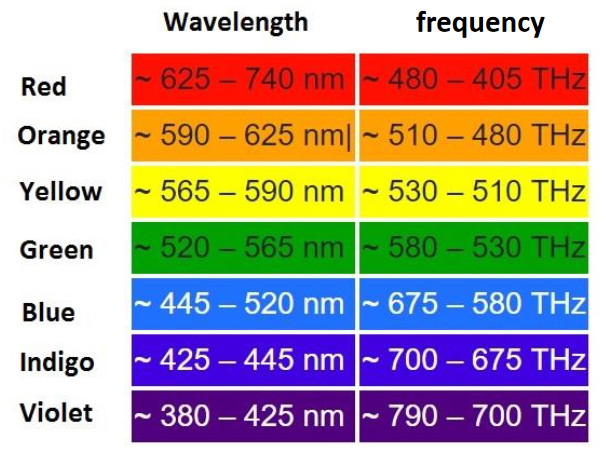
\includegraphics[width=0.5\textwidth]{immagini/spettro_visibile}
\end{center}

\section{Luce come insieme di particelle}
La luce \`e fatta di fotoni, particelle senza massa che viaggiano alla velocit\`a della luce.
Un fascio di luce \`e un insieme di fotoni, ciascuno con la propria frequenza, energia e
colore. Il colore del fascio di luce dipende da come l'insieme di fotoni \`e distribuito sullo
spettro delle frequenze. A noi interessa in particolare questo modo di vedere la luce.

\section{Percezione del colore}
Gli oggetti non hanno un colore, hanno delle propriet\`a fisiche e la luce viene riflessa in
base
\begin{itemize}
	\item alle propriet\`a dei materiali di cui \`e composto l'oggetto.
	\item alle caratteristiche della luce.
	\item al colore intorno all'oggetto.
	\item alla percezione dell'osservatore.
\end{itemize}
La nostra percezione della luce \`e \textbf{additiva}. Se ho quindi due luci di colore diverso
che si sovrappongono vedo la combinazione delle due. Se ho tutti e tre i colori primari insieme
vedo una luce bianca.

Noi vediamo meglio la luce con lunghezza d'onda intorno ai 550nm, ovvero vediamo questi colori
come pi\`u luminosi. La \textbf{funzione di efficienza luminosa fotopica} ce lo mostra.
\begin{center}
	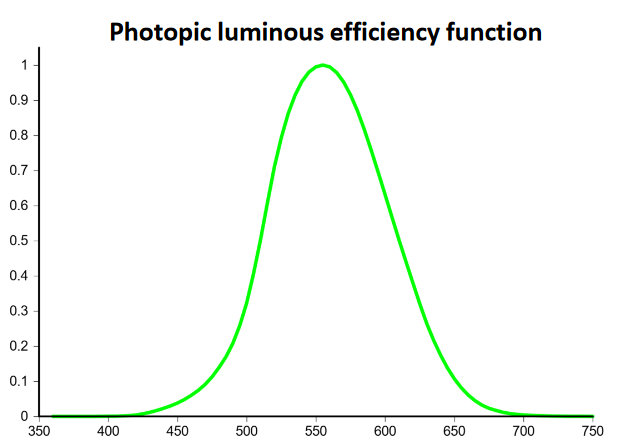
\includegraphics[width=0.5\textwidth]{immagini/funzione_fotopica}
\end{center}
Se ho una luce, per sapere come la percepisco, la moltiplico in ogni punto per la funzione
fotopica.

\section{Coefficienti tricromatici e valori RGB}
Se io dovessi regolare tre manopole, una che regola l'intenst\`a del rosso, una del verde e
una del blu e volessi ottenere una luce bianca alla fine avrei tre valori diversi per ogni
manopola, diciamo $r, g, b$. Quello che vogliamo, per\`o, \`e che il bianco, che \`e la somma
di tutti i colori, sia effettivamente rappresentato come combinazione dei tre colori (rosso,
verde e blu) ognuno col massimo valore e soprattutto vogliamo che questo valore sia uguale
per tutti e 3 i colori. Non devono perci\`o dipendere dalla nostra percezione.

Se volessi rappresentare il tutto con un'equazione sarebbe cos\`i.
\[ Bianco = r \cdot m_r \oplus g \cdot m_g \oplus b \cdot m_b \]
dove $a \oplus b$ indica la percezione delle luci $a$ e $b$ sovrapposte e dove
$m_r, m_g, m_b$ sono delle costanti che valgono
\[ m_r = 1 \quad m_g = 4.39 \quad m_b = 0.0048 \]
l'obbiettivo \`e quello di ottenere
\[ r \cdot m_r = g \cdot m_g = b \cdot m_b \]
Ecco che entrano in gioco i \textbf{coefficienti tricromatici} definiti come segue
\begin{gather*}
	\alpha = \frac{r \cdot m_r}{r \cdot m_r + g \cdot m_g + b \cdot m_b} \\
	\\
	\beta = \frac{g \cdot m_g}{r \cdot m_r + g \cdot m_g + b \cdot m_b} \\
	\\
	\gamma = \frac{b \cdot m_b}{r \cdot m_r + g \cdot m_g + b \cdot m_b}
\end{gather*}
A questo punto ho che il generico colore $C$ \`e dato da
\[ C = \alpha \oplus \beta \oplus \gamma \]
vale inoltre che
\[ \alpha + \beta + \gamma = 1 \]
Questo procedimento ha come risultato quello di non considerare la \emph{luminanza} e tenere
di conto solo la mistura di colori nella stessa misura per ogni primario.

Se volessimo invece ottenere la luminanza di un certo colore, sapendo i suoi coefficienti
tricromatici dovremmo calcolare
\[ L = \alpha \cdot m_r + \beta \cdot m_g + \gamma \cdot m_b \]

Ma come facciamo a ottenere i valori RGB di un colore non spettrale ?
Dobbiamo sapere quanto rosso, quanto verde e quanto blu mettere. La "quantit\`a" di colore che
dobbiamo mettere \`e data dalle seguenti sommatorie
\begin{gather*}
	R = \sum_{\lambda = 380}^{\lambda = 780} \overline{r}(\lambda) E(\lambda) \\
	\\
	G = \sum_{\lambda = 380}^{\lambda = 780} \overline{g}(\lambda) E(\lambda) \\
	\\
	B = \sum_{\lambda = 380}^{\lambda = 780} \overline{b}(\lambda) E(\lambda) \\
\end{gather*}
Dove le funzioni soprasegnate sono la \emph{color matching function} dello specifico colore,
ovvero quanto di quel colore vedo ad una determinata frequenza della luce, nel punto
$\lambda$ mentre $E(\lambda)$ equivale all'energia che arriva nello spettro.

\section{Spazi di colori}
Per ottenere sfumature di colore in modo pi\`u agevole sono stati introdotti
degli \textbf{spazi di colori}.

\subsection{HSV}
L'HSV (\textbf Hue, \textbf Saturation and \textbf Value) funziona in questo modo:
\begin{itemize}
	\item Il primo valore \`e la tinta, il colore scelto.
	\item Il secondo valore \`e la saturazione e l'idea \`e quella di impostare con essa,
	      quanto grigio si vuole aggiungere al colore scelto. Se la saturazione \`e
	      massima non aggiunger\`o grigio al mio colore, se \`e minima otterr\`o proprio
	      il grigio. Il valore minimo \`e 0 e il valore massimo \`e 1 ma questi valori
	      dipendono in modo proporzionale dal prossimo valore.
	\item Il terzo valore \`e la luminosit\`a del grigio che sto aggiungendo al mio colore.
	      Con il valore massimo otterr\`o il bianco, con il minimo otterr\`o il nero
	      (valore minimo 0, valore massimo 1).
\end{itemize}

\subsection{HSL}
L'HSL (\textbf Hue, \textbf Saturation and \textbf Lightness) molto simile al precedente. In
questo caso abbiamo il valore della \textbf{luminosit\`a} che va da $-0.5$ a $0.5$ in questo
caso la saturazione \`e massima con luminosit\`a 0 e si abbassa se la luminosit\`a cala o
incrementa.
\documentclass[12pt, a4paper]{report}

\usepackage[T1]{fontenc}
\usepackage[italian]{babel}
\usepackage{mathtools, amsmath, amssymb, amsthm}
\usepackage[hidelinks]{hyperref}

\title{Algebra Lineare}
\author{Federico Bustaffa}
\date{13/02/2022}

\theoremstyle{definition}
\newtheorem{definition}{Definizione}[subsection]
\newtheorem{observation}[definition]{Osservazione}
\newtheorem{theorem}[definition]{Teorema}
\newtheorem{proposition}[definition]{Proposizione}
\newtheorem{lemma}[definition]{Lemma}
\newtheorem{example}[definition]{Esempio}
\newtheorem{corollary}[definition]{Corollario}

\newcommand{\K}{\mathbb{K}}
\newcommand{\Q}{\mathbb{Q}}
\newcommand{\R}{\mathbb{R}}
\newcommand{\Z}{\mathbb{Z}}
\newcommand{\B}{\mathcal{B}}

\DeclareMathOperator{\Imm}{Imm}
\DeclareMathOperator{\Mat}{Mat}
\DeclareMathOperator{\Ker}{Ker}

\begin{document}

\maketitle
\tableofcontents

\chapter{Spazi Vettoriali}

\section{Definizione di spazio vettoriale}
Per fornire la definizione di spazio vettoriale si ha bisogno di un insieme non vuoto $V$ e di un campo
$\K$, dove sia possibile definire le operazioni di \textbf{somma vettoriale} e
\textbf{prodotto per scalare}.

\begin{definition}
	Uno \textbf{spazio vettoriale su un campo} $\K$ è un insieme $V$ su cui sono definite la somma
	fra due elementi di $V$ (il cui risultato è ancora un elemento di V, si dice quindi che $V$ è chiuso
	per la somma), e il prodotto di un elemento di $\K$ per un elemento di $V$ (il cui risultato è
	sempre un elemento di $V$, si dice quindi che V è chiuso per il prodotto con elementi di $\K$)
	che verificano le seguenti \textbf{proprietà}:
	\begin{enumerate}
		\item \textbf{Associatività della somma}: $\forall u, v, w \in V$ vale
		      \[ (u + v) + w = u + (v + w) \]
		\item \textbf{Commutatività della somma}: $\forall v, w \in V$ vale
		      \[ v + w = w + v \]
		\item \textbf{Elemento neutro per la somma}: $\exists O \in V$ tale che $\forall v \in V$ vale
		      \[ v + O = v \]
		\item \textbf{Inverso per la somma}: $\forall v \in V$, $\exists w \in V$ tale che
		      \[ v + w = O \]
		\item \textbf{Distributività del prodotto per uno scalare}: $\forall \lambda, \mu \in \K$ e
		      $\forall v, w \in V$ vale
		      \[ \lambda(v + w) = \lambda v + \lambda w \]
		      e anche
		      \[ (\lambda + \mu)v = \lambda v + \mu v \]
		\item \textbf{Associatività del prodotto per uno scalare}: $\forall \lambda, \mu \in \K$ e
		      $\forall v \in V$ vale
		      \[ (\lambda \mu)v = \lambda(\mu v) \]
		\item \textbf{Invariante moltiplicativo}: $\forall v \in V$ vale
		      \[ 1v = v \]
	\end{enumerate}
\end{definition}

\begin{observation}
	L'elemento neutro della somma $O$ e lo $0$, elemento neutro di $\K$ sono due cose ben distinte, il primo è
	un vettore, il secondo è uno scalare.
\end{observation}

\begin{example}
	Ogni campo $\K$ è uno spazio vettoriale su $\K$ stesso con le operazioni di somma vettoriale e prodotto per
	scalare che sono definite identiche alle operazioni di somma e prodotto sul campo. In particolare $\R$ è uno
	spazio vettoriale su $\R$, così come $\Q$ è uno spazio vettoriale su $\Q$.
\end{example}

\begin{example}
	$\R^2 = \{(a, b) \mid a,b \in \R\}$ è uno spazio vettoriale su $\R$ con le operazioni di somma vettoriale e
	prodotto scalare definite come segue:
	\begin{align*}
		(a,b) + (c,d) =  & (a + c, b + d)         \\
		\lambda (a, b) = & (\lambda a, \lambda b)
	\end{align*}
\end{example}

\begin{example}
	Anche l'insieme dei polinomi $\K[x]$, con la somma tra polinomi e il prodotto tra polinomi e costanti di
	$\K$ definiti come segue:
	\begin{itemize}
		\item Il polinomio somma di $p(x)$ e $q(x)$ è quello il cui coefficiente di grado $n$ è la somma dei
		      coefficienti di grado $n$ dei polinomi $p(x)$ e $q(x)$.
		\item Il polinomio prodotto di $k \in \K$ e $p(x)$ è il polinomio che ha come coefficiente di
		      grado $n$ $k$ volte il coefficiente di grado $n$ di $p(x)$.
	\end{itemize}
	è uno spazio vettoriale su $\K$.
\end{example}

\section{Sottospazi vettoriali}

\begin{definition}
	Un \textbf{sottospazio vettoriale} $W$ di $V$ è un sottoinsieme di $V$ che (rispetto alle operazioni $+$
	e $\cdot$ che rendono $V$ uno spazio vettoriale su $\K$) è uno spazio vettoriale su $\K$.
\end{definition}

\begin{example}
	Dato uno spazio vettoriale $V$ su un campo $\K$, $V$ e l'insieme ${O}$ sono sempre sottospazi di $V$.
\end{example}

\begin{definition}
	Chiamiamo \textbf{sottospazio proprio} di $V$ un qualsiasi sottospazio vettoriale di $V$ che sia diverso da
	$V$ e dal sottospazio ${O}$.
\end{definition}

\begin{proposition}
	Dato uno spazio vettoriale $V$ su $\K$ e $W \subseteq V$, $W$ è sottospazio vettoriale di $V$
	(rispetto alle operazioni $+$ e $\cdot$ che rendono $V$ uno spazio vettoriale su $\K$) se e solo
	se:
	\begin{enumerate}
		\item Il vettore $O$ appartiene a $W$.
		\item $\forall u, v \in W$ vale $u + v \in W$.
		\item $\forall k \in \K$ e $\forall u \in W$ vale $ku \in W$.
	\end{enumerate}
\end{proposition}

\begin{example}
	Consideriamo lo spazio vettoriale $\R^2$ su $\R$ e proviamo vedere se l'insieme
	$X = \{\forall x,y \in \R \mid x^2 + y^2 = 1\}$ è un sottospazio vettoriale di $\R^2$.
	L'insieme in questione è l'insieme di punti di una circonferenza. Subito notiamo che il vettore $(0, 0)$
	non appartiene all'insieme dunque possiamo subito concludere che $X$ non è un sottospazio di
	$\R^2$.
\end{example}

\begin{observation}
	Tutte le rette passanti per l'origine sono gli unici sottospazi vettoriali di $\R^2$. Tutti gli altri
	sottoinsiemi non sono chiusi per somma e prodotto.
\end{observation}

\begin{example}
	Consideriamo il sottoinsieme $L$ di $\K[x]$ che contiene tutti e soli i polinomi che hanno radice
	$1$, ovvero:
	\[ L = \{p(x) \in \K[x] \mid p(1) = 0\} \]
	Verifichiamo che $L$ è sottospazio vettoriale di $\K[x]$.
	\begin{itemize}
		\item Il polinomio $0$, che è il vettore $O$ di $\K[x]$, appartiene a $L$, infatti ha $1$
		      come radice (addirittura ogni elemento di $\K$ è una radice di $0$).
		\item Se $p(x), q(x) \in L$ allora $(p + q)(x)$ appartiene a $L$, infatti:
		      \[ (p + q)(1) = p(1) + q(1) = 0 + 0 = 0 \]
		\item Se $p(x) \in L$ e $k \in \K$ allora $k \cdot p(x) \in L$, infatti:
		      \[ (k \cdot p)(1) = k \cdot p(1) = k \cdot 0 = 0 \]
	\end{itemize}
\end{example}

\section{Intersezione e somma di sottospazi vettoriali}
Dati due sottospazi vettoriali $U$ e $W$ di uno spazio vettoriale $V$, la somma è il più piccolo sottospazio
vettoriale di $V$ che contenga sia $U$ che $W$ mentre l'intersezione è il più grande sottospazio vettoriale
di $V$ contenuto sia in $U$ che in $W$.

\begin{proposition}
	Sia $V$ uno spazio vettoriale su un campo $\K$, $U$ e $W$ due sottospazi di $V$, allora $U \cap W$
	è un sottospazio vettoriale di $V$.
	\begin{proof}
		Ci interessa verificare che $U \cap W$ verifichi le proprietà della definizione:
		\begin{enumerate}
			\item $O \in U \cap W$, infatti essendo $U$ e $W$ due sottospazi, certamente $O \in U$ e $O \in W$.
			\item Siano $v_1, v_2 \in U \cap W$ allora:
			      \[
				      \begin{cases}
					      v_1 + v_2 \in U \\
					      v_1 + v_2 \in W
				      \end{cases}
				      \Rightarrow{v_1 + v_2 \in U \cap W}
			      \]
			\item Sia $v \in U \cap W$ allora $\forall \lambda \in \K$ si ha:
			      \[
				      \begin{cases}
					      \lambda v \in U \\
					      \lambda v \in W
				      \end{cases}
				      \Rightarrow{\lambda v \in U \cap W}
			      \]
		\end{enumerate}
	\end{proof}
\end{proposition}

Per cercare il più piccolo sottospazio contenente sia $U$ che $W$ verrebbe da pensare all'unione insiemistica,
tuttavia, in generale non è vero che $U \cup W$ è un sottospazio vettoriale di $V$.

Dunque il più piccolo sottospazio vettoriale di $V$ che contiene sia $U$ che $W$ deve necessariamente (per
essere chiuso per la somma) contenere tutti gli elementi della forma $u + v$ dove $u \in U$ e $w \in W$.

\begin{example}
	Provare che se $V = \R^2$ e $U$ e $W$ sono due rette distinte passanti per $O$, allora $U \cup W$
	non è un sottospazio di $V$.

	Basta mostrare che, presi $u \in U$ e $w \in W$, entrambi diversi dall'origine, $v + w$ non appartiene
	all'unione $U \cup W$.
\end{example}

\begin{definition}
	Dati due sottospazi vettoriali $U$ e $W$ di uno spazio vettoriale $V$ su $\K$, chiamo \textbf{somma}
	di $U$ e $W$ l'insieme
	\[ U + W = \{u + w \mid u \in U, w \in W\} \]
\end{definition}

\begin{proposition}
	Dati due sottospazi vettoriali $U$ e $W$ di uno spazio vettoriale $V$ su $\K$, $U + W$ è un
	sottospazio vettoriale di $V$ (ed è il più piccolo contenente $U$ e $W$).
	\begin{proof}
		Partiamo col dire che $O \in U + W$, infatti $O$ appartiene sia ad $U$ che a $W$. Ora, dati
		$a \in \K$ e $x, y \in U + W$, per definizione di $U + W$ esistono $u_1, u_2 \in U$ e
		$w_1, w_2 \in W$ tali che
		\begin{align*}
			x = & u_1 + w_1 \\ y = & u_2 + w_2
		\end{align*}
		Dunque
		\[ x + y = (u_1 + w_1) + (u_2 + w_2) = (u_1 + u_2) + (w_1 + w_2) \in U + W \]
		e
		\[ ax = a(u_1 + w_1) = au_1 + aw_1 \in U + W \]
	\end{proof}
\end{proposition}


% BASI

\subsection{Base di uno spazio vettoriale}
Sia $V$ uno spazio vettoriale su $\mathbb{K}$.
Per definizione di $V$, se $v_1, v_2, ..., v_n$ sono $n$ vettori
di $V$, allora per qualsiasi scelta di $n$ elementi
$k_1, k_2, ..., k_n$ di $\mathbb{K}$ il vettore:
\begin{equation*}
	v = k_1 v_1 + ... + k_n v_n = \sum_{i=1}^n k_i v_i
\end{equation*}
appartiene a $V$, in quanto $V$ \`e chiuso per somma vettoriale
e prodotto per scalare.

\begin{defn}
	Dato un insieme di vettori $\{v_1, v_2, ..., v_n\}$ di $V$,
	spazio vettoriale sul campo $\mathbb{K}$, il vettore:
	\begin{equation*}
		v = k_1 \cdot v_1 + ... + k_n \cdot v_n
	\end{equation*}
	con $\{k_1, k_2, ..., k_n\}$ scalari di $\mathbb{K}$,
	si dice una \textbf{combinazione lineare} dei vettori
	$\{v_1, v_2, ..., v_n\}$. I $k_i$ sono detti \textbf{coefficienti}
	della combinazione lineare.
\end{defn}

\begin{example}
	Consideriamo lo spazio vettoriale $\mathbb{R}^3$ su $\mathbb{R}$ e i seguenti
	due vettori:
	\begin{equation*}
		v_1 = \begin{pmatrix}
			3 \\ -1 \\ 3
		\end{pmatrix}
		\quad
		v_2 = \begin{pmatrix}
			1 \\ 0 \\ 2
		\end{pmatrix}
	\end{equation*}
	Allora il vettore $v_3$ seguente:
	\begin{equation*}
		v_3 = \begin{pmatrix}
			5 \\ -1 \\ 7
		\end{pmatrix}
		= 1 \cdot \begin{pmatrix}
			3 \\ -1 \\ 3
		\end{pmatrix}
		+ 2 \cdot \begin{pmatrix}
			1 \\ 0 \\ 2
		\end{pmatrix}
	\end{equation*}
	\`E una combinazione lineare dell'insieme dei vettori $\{v_1, v_2\}$ di
	coefficienti 1 e 2.
\end{example}

\begin{defn}
	Dati $\{v_1, v_2, ..., v_t\}$ vettori di $V$ su $\mathbb{K}$,
	si definisce \textbf{span} dei vettori $v_1, v_2, ..., v_t$
	(e si indica con $Span(v_1, v_2, ..., v_t)$) l'insieme di tutte
	le possibili combinazioni lineari dell'insieme di vettori
	$\{v_1, v_2, ..., v_t\}$.
\end{defn}

\begin{defn}
	Un insieme di vettori $\{v_1, v_2, ..., v_t\}$ di $V$ per cui
	$V = Span(v_1, v_2, ..., v_t)$, ovvero $\forall v \in V$, esistono
	degli scalari $a_1, a_2, ..., a_t$ tali che
	\begin{equation*}
		a_1 v_1 + a_2 v_2 + ... + a_t v_t = v
	\end{equation*}
	si dice un \textbf{insieme di generatori} di $V$. In tal caso si dice
	anche che i vettori $v_1, v_2, ..., v_t$ \textbf{generano} $V$.
\end{defn}

L'esistenza di un sistema finito di generatori per uno spazio vettoriale
$V$ su un campo $\mathbb{K}$ \`e un fatto molto importante, dato che
si riduce la descrizione di uno spazio vettoriale con cardinalit\`a
infinita, ad una lista di numero finito di vettori di $V$.


Dato un sistema di generatori $\{v_1, ..., v_t\}$ di $V$ sappiamo dunque
che ogni $v \in V$ si pu\`o scrivere, con opportuni coefficienti
$\{k_1, ..., k_t\}$, come:
\begin{equation*}
	v = \sum_{i=1}^t k_i v_i
\end{equation*}
In generale, tale scrittura non \`e unica, ovvero non ci permette di
identificare univocamente ogni vettore di $v \in V$.

\begin{example}
	Si verifica che i vettori
	\begin{equation*}
		\begin{pmatrix}
			1 \\ 2 \\ 3
		\end{pmatrix} \quad
		\begin{pmatrix}
			1 \\ 0 \\ 1
		\end{pmatrix} \quad
		\begin{pmatrix}
			0 \\ 0 \\ 1
		\end{pmatrix} \quad
		\begin{pmatrix}
			2 \\ 2 \\ 4
		\end{pmatrix}
	\end{equation*}

	generano $\mathbb{R}^3$. Si possono facilmente trovare due distinte
	combinazioni lineari di tali vettori che esprimono il vettore
	\begin{equation*}
		\begin{pmatrix}
			2 \\ 2 \\ 5
		\end{pmatrix}
	\end{equation*}

	Per esempio:
	\begin{equation*}
		\begin{pmatrix}
			1 \\ 2 \\ 3
		\end{pmatrix} +
		\begin{pmatrix}
			1 \\ 0 \\ 1
		\end{pmatrix} +
		\begin{pmatrix}
			0 \\ 0 \\ 1
		\end{pmatrix} =
		\begin{pmatrix}
			2 \\ 2 \\ 5
		\end{pmatrix} =
		\begin{pmatrix}
			2 \\ 2 \\ 4
		\end{pmatrix} +
		\begin{pmatrix}
			0 \\ 0 \\ 1
		\end{pmatrix}
	\end{equation*}
\end{example}

\begin{defn}
	Si dice che un insieme finito di vettori $\{v_1, v_2, ..., v_r\}$ \`e
	un \textbf{insieme di vettori linearmente indipendenti} se l'unico
	modo di scrivere il vettore $O$ come combinazione lineare di questi
	vettori \`e con tutti i coefficienti nulli, ossia se
	\begin{equation*}
		a_1 v_1 + a_2 v_2 + ... + a_r v_r = O \quad \Leftrightarrow \quad
		a_1 = a_2 = ... = a_r = 0
	\end{equation*}
	Si pu\`o dire anche che i vettori sono \textbf{linearmente indipendenti}.
	Se invece i vettori $v_1, v_2, ..., v_r$ non sono linearmente indipendenti
	si dice che sono \textbf{linearmente dipendenti}.
\end{defn}

\begin{proposition}
	Un insieme $A = \{v_1, ..., v_n\}$ di vettori di uno spazio
	vettoriale $V$ su $\mathbb{K}$ \`e un insieme di vettori linearmente
	indipendenti se e solo se nessun $v_i$, appartenente ad $A$, si pu\`o
	scrivere come combinazione lineare dell'insieme
	$B = A \backslash \{v_i\}$ (ovvero $v_i$ non appartiene a $Span(B)$).
\end{proposition}

\begin{defn}
	Sia $V$ uno spazio vettoriale su $\mathbb{K}$, un insieme di vettori
	$\{v_1, v_2, ..., v_n\} \in V$, che generano lo spazio $V$ e che sono
	linearmente indipendenti, si dice una \textbf{base} (finita) di $V$.
\end{defn}

\begin{observation}
	Nella definizione \`e specificato \emph{finita}. Non sempre uno
	spazio vettoriale ammette un numero finito di generatori, e di
	conseguenza nemmeno una base finita.
\end{observation}

Fissata la defizione di base siamo interessati a capire:
\begin{enumerate}
	\item
	      Se la scelta di una base garantisce l'unicit\`a di scrittura di un vettore
	      in termini di combinazione lineare degli elementi della base.
	\item
	      Quando uno spazio vettoriale ammette una base finita, ed in
	      particolare se il fatto che uno spazio vettoriale $V$ abbia un
	      insieme finito di generatori, garantisca che $V$ abbia una
	      base finita o meno.
\end{enumerate}

\begin{proposition}
	Ogni vettore $v \in V$ si scrive \emph{in modo unico} come
	combinazione lineare degli elementi della base.
\end{proposition}

\begin{theorem}
	Sia $V$ uno spazio vettoriale su $\mathbb{K}$ diverso da $\{O\}$
	e generato dall'insieme finito di vettori \emph{non nulli}
	$\{w_1, w_2, ..., w_s\}$. Allora \`e possibile estrarre da
	$\{w_1, w_2, ..., w_s\}$ un sottoinsieme
	$\{w_{i_1}, w_{i_2}, ..., w_{i_n}\}$ (con $n \leq s$) che \`e
	una base di $V$.
\end{theorem}

\begin{defn}
	Sia $V$  uno spazio vettoriale con basi di cardinalit\`a $n$.
	Tale cardinalit\`a $n$ \`e detta \textbf{dimensione} di $V$.
\end{defn}

\section{Applicazioni Lineari}
Le applicazioni lineari non sono altro che funzioni che mandano sottospazi in sottospazi.

\begin{example}
	Consideriamo la funzione $\textit{f} : \R^2 \to \R^2$ definita da
	\[
		f \begin{pmatrix}
			x \\ y
		\end{pmatrix}
		=
		\begin{pmatrix}
			x \\ x^2
		\end{pmatrix}
	\]
	La funzione $f$ manda il punto $(x, x)$, con la prima e seconda coordinata uguali, ovvero i punti della
	retta di equazione $x = y$, nella parabola di equazione $y = x^2$. Ma, come sappiamo, la retta $y = x$,
	passando dall'origine, è un sottospazio di $\R^2$, mentre la parabola non lo è. Si devono dunque
	considerare applicazioni con proprietà particolari.
\end{example}

\begin{definition}
	Siano $V$ e $W$ spazi vettoriali di dimensione finita sul campo $\K$. Un'applicazione $L$ da $V$
	in $W$ è detta \textbf{lineare} se soddisfa le seguenti proprietà:
	\begin{itemize}
		\item $\forall v_1, v_2 \in V$ vale
		      \[ L(v_1 + v_2) = L(v_1) + L(v_2) \]
		\item $\forall \lambda \in \K$ e $\forall v \in V$ vale
		      \[ L(\lambda v) = \lambda L(v) \]
	\end{itemize}
\end{definition}

\begin{observation}
	Soddisfare le due proprietà, da parte di un'applicazione lineare $L$, è equivalente a soddisfare la seguente
	proprietà: $\forall v_1, v_2 \in V$ e $\forall \lambda, \mu \in \K$ vale
	\[ L(\lambda v_1 + \mu v_2) = \lambda L(v_1) + \mu L(v_2) \]
\end{observation}

\begin{definition}
	Siano $V$ e $W$ spazi vettoriali su $\K$ e $L$ un'applicazione lineare da $V$ in $W$. Chiamo
	\textbf{immagine} di $L$, e la indico con $\Imm(L)$, il seguente sottoinsieme di $W$:
	\[ \Imm(L) = \{w \in W \mid \forall v \in V, \quad L(v) = w\} \]
\end{definition}

\begin{proposition}
	È dimostrabile che \[ \Imm(L) = Span(L(e_1), \dots, L(e_n)) \] dove $\{e_1, \dots, e_n\}$ è una base di $V$.
\end{proposition}

\begin{definition}
	Siano $V$ e $W$ spazi vettoriali su $\K$ e $L$ un'applicazione lineare da $V$ in $W$. Chiamo
	\textbf{nucleo} di $L$, e lo indico con $\Ker(L)$, il seguente sottoinsieme di $V$:
	\[ \Ker(L) = \{v \in V \mid L(v) = O\} \]
\end{definition}

Di seguito qualche proprietà utile:
\begin{enumerate}
	\item $\Ker(L)$ è un sottospazio vettoriale di $V$.
	\item $\Imm(L)$ è un sottospazio vettoriale di $W$.
	\item $L$ è iniettiva se e solo se $\Ker(L) = \{O\}$.
\end{enumerate}



% MATRICI E VETTORI

\subsection{Matrici e vettori}

\begin{defn}
	Dati due interi positivi $m, n$, una \textbf{matrice} $m \times n$
	a coefficienti in $\mathbb{K}$ \`e una griglia composta da $m$ righe
	e $n$ colonne in cui in ogni posizione c'\`e un elemento di
	$\mathbb{K}$:
	\begin{equation*}
		A = \begin{pmatrix}
			a_{11} & a_{12} & \dots & a_{1n} \\
			a_{21} & a_{22} & \dots & \dots  \\
			\dots  & \dots  & \dots & \dots  \\
			a_{m1} & \dots  & \dots & a_{mn}
		\end{pmatrix}
	\end{equation*}
	Per indicare l'elemento che si trova nella riga $i$-esima
	dall'alto e	nella colonna $j$-esima da sinistra viene indicato
	con $a_{ij}$. Spesso per indicare la matrice $A$ useremo la notazione
	$A = (a_{ij})$ e per ricordare le dimensioni della matrice scriveremo:
	\begin{equation*}
		A = (a_{ij})_{\substack{
					i = 1, 2, \dots, m \\
					j = 1, 2, \dots, n
				}}
	\end{equation*}
\end{defn}

\begin{defn}
	Dati due interi positivi m, n, chiamiamo
	$Mat_{m \times n} (\mathbb{K})$, l'insieme di tutte le matrici
	$m \times n$ a coefficienti in $\mathbb{K}$.
\end{defn}

\begin{defn}
	Sull'insieme $Mat_{m \times n} (\mathbb{K})$ possiamo definire la
	\textbf{somma} e il \textbf{prodotto per scalare}. Date due matrici
	$A, B \in Mat_{m \times n} (\mathbb{K})$ e dato uno scalare
	$k \in \mathbb{K}$, definiamo:
	\begin{itemize}
		\item
		      La \textbf{matrice somma} $A + B = C$, il cui generico coefficiente nella
		      $i$-esima riga e $j$-esima colonna si ottiene sommando i
		      coefficienti nella stessa posizione indicata da $(i, j)$ di $A$ e
		      di $B$. Ovvero per ogni $i \leq m$ e per ogni $j \leq n$
		      ho che $c_{ij} = a_{ij} + b_{ij}$.
		\item
		      La \textbf{matrice prodotto per scalare} $k \cdot A = D$, il cui
		      generico coefficiente nella $i$-esima riga e $j$-esima
		      colonna si ottiene moltiplicando lo scalare $k$ per il
		      coefficiente di $A$ in posizione $(i, j)$. Ovvero per ogni
		      $i \leq m$ e per ogni $j \leq n$ ho che
		      $d_{ij} = k \cdot a_{ij}$.
	\end{itemize}
\end{defn}

Esiste un'altra operazione, si tratta del
\emph{prodotto righe per colonne}. Per definire tale prodotto \`e
importante l'ordine in cui si considerano le due matrici (quindi non vale la
proprit\`a commutativa). Inoltre tale operazione \`e definita solo quando il
numero di colonne di $A$ \`e uguale al numero di righe di $B$.

\begin{defn}
	Data una matrice $A = (a_{ij}) \in Mat_{m \times n} (\mathbb{K})$ e una
	matrice $B = (b_{st}) \in Mat_{n \times k} (\mathbb{K})$, il
	\textbf{prodotto riga per colonna} $AB$, \`e la matrice
	$C = (c_{rh}) \in Mat_{m \times k} (\mathbb{K})$, i cui coefficienti,
	per ogni $r, h$, sono definiti come segue:
	\begin{equation*}
		c_{rh} = a_{r1} b_{1h} + a_{r2} b_{2h} + \cdots + a_{rn} b_{nh}
	\end{equation*}
\end{defn}

\begin{example}
	Consideriamo la matrice $A \in Mat_{2 \times 3}(\mathbb{K})$:
	\begin{equation*}
		A = \begin{pmatrix}
			1 & 2 & 4 \\
			0 & 6 & 3
		\end{pmatrix}
	\end{equation*}
	e la matrice $B \in Mat_{3 \times 3}(\mathbb{K})$:
	\begin{equation*}
		B = \begin{pmatrix}
			2 & 2 & 2  \\
			5 & 6 & -8 \\
			0 & 1 & 0
		\end{pmatrix}
	\end{equation*}
	La definizione ci dice che possiamo definire $C = AB$ e che $C$ \`e la matrice di
	$Mat_{2 \times 3}(\mathbb{K})$ i cui coefficienti sono ottenuti come segue:
	\begin{gather*}
		c_{11} = 1 \cdot 2 + 2 \cdot 5 + 4 \cdot 0 = 12 \\
		c_{12} = 1 \cdot 2 + 2 \cdot 6 + 4 \cdot 1 = 18 \\
		c_{13} = 1 \cdot 2 + 2 \cdot (-8) + 4 \cdot 0 = -14 \\
		c_{21} = 0 \cdot 2 + 6 \cdot 5 + 3 \cdot 0 = 30 \\
		c_{22} = 0 \cdot 2 + 6 \cdot 6 + 3 \cdot 1 = 39 \\
		c_{23} = 0 \cdot 2 + 6 \cdot (-8) + 3 \cdot 0 = -48
	\end{gather*}
	E dunque si ha:
	\begin{equation*}
		AB = C = \begin{pmatrix}
			12 & 18 & -14 \\
			30 & 39 & -48
		\end{pmatrix}
	\end{equation*}
\end{example}

\begin{defn}
	Data un'applicazione lineare $L$ da uno spazio vettoriale $V$ di
	dimensione $n$ ad uno spazio vettoriale $W$ di dimensione $m$, si dice
	\textbf{matrice associata} all'applicazione lineare $L$ nelle basi
	$\{e_1, e_2, \dots, e_n\}$ di $V$ e
	$\{\epsilon_1, \epsilon_2, \dots, \epsilon_m\}$ di $W$, la seguente
	matrice di $m$ righe ed $n$ colonne:
	\begin{equation*}
		[L]_{\substack{
				e_1, e_2, \dots, e_n\\
				\epsilon_1, \epsilon_2, \dots, \epsilon_m
			}} = \begin{pmatrix}
			a_{11} & a_{12} & \dots & a_{1n} \\
			a_{21} & a_{22} & \dots & \dots  \\
			\dots  & \dots  & \dots & \dots  \\
			a_{m1} & \dots  & \dots & a_{mn}
		\end{pmatrix}
	\end{equation*}
	dove $\{e_1, e_2, \dots, e_n\}$ \`e la base di partenza e
	$\{\epsilon_1, \epsilon_2, \dots, \epsilon_m\}$ \`e la base di arrivo.
\end{defn}

Sar\`a tutto pi\`u chiaro con un esempio che vedremo tra poco. In ogni caso, per
alleggerire la notazione, si possono omettere le basi, tuttavia si deve ricordare che
la matrice $[L]$ associata all'applicazione lineare $L$, non dipende solo da $L$ stessa,
ma anche dalle basi scelte per $V$ e $W$.

\begin{example}
	Consideriamo gli spazi vettoriali $\mathbb{R}^4$ con la sua base
	\begin{equation*}
		v_1 = \begin{pmatrix}
			1 \\ 1 \\ 0 \\ 0
		\end{pmatrix} \quad
		v_2 = \begin{pmatrix}
			0 \\ 1 \\ 1 \\ 0
		\end{pmatrix} \quad
		v_3 = \begin{pmatrix}
			0 \\ 0 \\ 1 \\ 1
		\end{pmatrix} \quad
		v_4 = \begin{pmatrix}
			0 \\ 0 \\ 0 \\ 1
		\end{pmatrix}
	\end{equation*}
	e $\mathbb{R}^3$ con la sua base
	\begin{equation*}
		w_1 = \begin{pmatrix}
			1 \\ 0 \\ 1
		\end{pmatrix} \quad
		w_2 = \begin{pmatrix}
			1 \\ 1 \\ 1
		\end{pmatrix} \quad
		w_3 = \begin{pmatrix}
			0 \\ 0 \\ 2
		\end{pmatrix}
	\end{equation*}
	Quel che vogliamo fare \`e scrivere la matrice associata all'applicazione lineare
	\begin{equation*}
		L \begin{pmatrix}
			x \\ y \\ z \\ w
		\end{pmatrix} = \begin{pmatrix}
			x + y + z \\
			y - z     \\
			x + w
		\end{pmatrix}
	\end{equation*}
	Procediamo calcolando l'immagine di ognuna delle componenti della base di
	$\mathbb{R}^4$
	\begin{gather*}
		L \begin{pmatrix}
			1 \\ 1 \\ 0 \\ 0
		\end{pmatrix} =
		\begin{pmatrix}
			2 \\ 1 \\ 1
		\end{pmatrix} \quad
		L \begin{pmatrix}
			0 \\ 1 \\ 1 \\ 0
		\end{pmatrix} =
		\begin{pmatrix}
			2 \\ 0 \\ 0
		\end{pmatrix} \\
		L \begin{pmatrix}
			0 \\ 0 \\ 1 \\ 1
		\end{pmatrix} =
		\begin{pmatrix}
			1 \\ -1 \\ 1
		\end{pmatrix} \quad
		L \begin{pmatrix}
			0 \\ 0 \\ 0 \\ 1
		\end{pmatrix} =
		\begin{pmatrix}
			0 \\ 0 \\ 1
		\end{pmatrix}
	\end{gather*}
	Ora dobbiamo esprimere i risultati trovati come combinazioni lineari della base di
	$\mathbb{R}^3$.
	\begin{gather*}
		\begin{pmatrix}
			2 \\ 1 \\ 1
		\end{pmatrix} =
		a \begin{pmatrix}
			1 \\ 0 \\ 1
		\end{pmatrix} +
		b \begin{pmatrix}
			1 \\ 1 \\ 1
		\end{pmatrix} +
		c \begin{pmatrix}
			0 \\ 0 \\ 2
		\end{pmatrix}\\
		\\
		\begin{pmatrix}
			2 \\ 0 \\ 0
		\end{pmatrix} =
		a \begin{pmatrix}
			1 \\ 0 \\ 1
		\end{pmatrix} +
		b \begin{pmatrix}
			1 \\ 1 \\ 1
		\end{pmatrix} +
		c \begin{pmatrix}
			0 \\ 0 \\ 2
		\end{pmatrix}\\
		\\
		\begin{pmatrix}
			1 \\ -1 \\ 1
		\end{pmatrix} =
		a \begin{pmatrix}
			1 \\ 0 \\ 1
		\end{pmatrix} +
		b \begin{pmatrix}
			1 \\ 1 \\ 1
		\end{pmatrix} +
		c \begin{pmatrix}
			0 \\ 0 \\ 2
		\end{pmatrix}\\
		\\
		\begin{pmatrix}
			0 \\ 0 \\ 1
		\end{pmatrix} =
		a \begin{pmatrix}
			1 \\ 0 \\ 1
		\end{pmatrix} +
		b \begin{pmatrix}
			1 \\ 1 \\ 1
		\end{pmatrix} +
		c \begin{pmatrix}
			0 \\ 0 \\ 2
		\end{pmatrix}
	\end{gather*}
	Ottengo dunque quattro sistemi.
	\begin{gather*}
		\begin{cases}
			a + b      & = 2 \\
			b          & = 1 \\
			a + b + 2c & = 1
		\end{cases}
		\quad
		\begin{cases}
			a + b      & = 2 \\
			b          & = 0 \\
			a + b + 2c & = 0
		\end{cases} \\
		\\
		\begin{cases}
			a + b      & = 1  \\
			b          & = -1 \\
			a + b + 2c & = 1
		\end{cases}
		\quad
		\begin{cases}
			a + b      & = 0 \\
			b          & = 0 \\
			a + b + 2c & = 2
		\end{cases}
	\end{gather*}
	Se li risolvo ottengo
	\begin{gather*}
		\begin{cases}
			a & = 1  \\
			b & = 1  \\
			c & = -1
		\end{cases}
		\quad
		\begin{cases}
			a & = 2  \\
			b & = 0  \\
			c & = -1
		\end{cases} \\
		\\
		\begin{cases}
			a & = 2  \\
			b & = -1 \\
			c & = 0
		\end{cases}
		\quad
		\begin{cases}
			a & = 0 \\
			b & = 0 \\
			c & = 1
		\end{cases}
	\end{gather*}
	Ora non devo fare altro che prendere i vettori
	\begin{equation*}
		\begin{pmatrix}
			1 \\ 1 \\ -1
		\end{pmatrix}
		\quad
		\begin{pmatrix}
			2 \\ 0 \\ -1
		\end{pmatrix}
		\quad
		\begin{pmatrix}
			2 \\ -1 \\ 0
		\end{pmatrix}
		\quad
		\begin{pmatrix}
			0 \\ 0 \\ -1
		\end{pmatrix}
	\end{equation*}
	e formare la matrice associata all'applicazione lineare $L$.
	\begin{equation*}
		[L]_{\substack{v_1, v_2, v_3, v_4 \\
				w_1, w_2, w_3}} =
		\begin{pmatrix}
			1  & 2  & 2  & 0  \\
			1  & 0  & -1 & 0  \\
			-1 & -1 & 0  & -1
		\end{pmatrix}
	\end{equation*}
\end{example}

\begin{observation}
	Dati due spazi vettoriali $V$ e $W$, esiste una sola applicazione
	lineare da $V$ a $W$ la cui matrice associata \`e indipendente dalle
	basi scelte. Questa \`e l'\emph{applicazione nulla}
	$\mathcal{O} : V \rightarrow W$ che manda ogni $v \in V$ in $O \in W$.
	Qualunque siano le basi scelte, la matrice associata avr\`a tutti
	i coefficienti uguali a $0$.
\end{observation}

\begin{observation}
	Consideriamo l'applicazione \emph{identit\`a} $I : V \rightarrow V$,
	che lascia fisso ogni elemento di $v: I(v) = v \forall v \in V$, e
	fissiamo la base $\mathcal{B}$ di $V$. Si verifica che la matrice
	$[I] = (a_{ij})$, associata ad $I$ rispetto a $\mathcal{B}$, sia in
	arrivo che in partenza, \`e la matrice quadrata di formato $n \times n$
	che ha tutti i coefficienti uguali a $0$ eccetto quelli sulla
	diagonale, che sono invece uguali a $1$.

	Tale matrice \`e l'elemento neutro rispetto alla moltiplicazione riga
	per colonna in $Mat_{n \times n}(\mathbb{K})$.

	In seguito useremo solo il simbolo $I$ per indicare sia la matrice identit\`a
	che	l'applicazione lineare $I$.
\end{observation}

\section{Riduzione a scalini}

\subsection{Operazioni elementari sulle colonne}
Consideriamo una generica matrice in $Mat_{m \times n}(\mathbb{K})$:
\begin{equation*}
	A = \begin{pmatrix}
		a_{11} & a_{12} & \dots & a_{1n} \\
		a_{21} & a_{22} & \dots & \dots  \\
		\dots  & \dots  & \dots & \dots  \\
		a_{m1} & \dots  & \dots & a_{mn}
	\end{pmatrix}
\end{equation*}
e i tre seguenti tipi di mossa sulle colonne, detti anche
\textbf{operazioni elementari sulle colonne}:
\begin{enumerate}
	\item si somma alla colonna $i$ la colonna $j$ moltiplicata per uno scalare
	      $\lambda$.
	\item si moltiplica la colonna $i$ per uno scalare $\lambda$
	\item si scambiano fra di loro due colonne $i$ e $j$.
\end{enumerate}

\begin{defn}
	La \textbf{profondit\`a} di una colonna \`e definita come la posizione
	occupata (contata dal basso) dal suo pi\`u alto coefficiente diverso da 0.
	Alla colonna nulla si assegna per convenzione profondit\`a uguale a 0.
\end{defn}

\begin{example}
	Consideriamo la seguente matrice:
	\begin{equation*}
		A = \begin{pmatrix}
			0            & 4 - \sqrt{3} & 0  \\
			\sqrt{3} + 1 & 0            & 0  \\
			-2           & -2           & -2
		\end{pmatrix}
	\end{equation*}
	In questo caso la prima colonna ha profodit\`a uguale a 2, la
	seconda colonna uguale a 3 mentre la terza ha profondit\`a uguale a 1.
\end{example}

\begin{defn}
	Una matrice $A \in Mat_{m \times n}(\mathbb{K})$, si dice
	\textbf{in forma a scalini per colonne} se rispetta le seguenti propriet\`a:
	\begin{itemize}
		\item leggendo la matrice da sinistra a destra, le colonne non nulle si
		      incontrano tutte prima delle colonne nulle.
		\item leggendo la matrice da sinistra a destra, le profondit\`a
		      delle sue colonne non nulle risultano strettamente
		      decrescenti.
	\end{itemize}
\end{defn}

\begin{example}
	Questi sono esempi di matrici in forma \emph{a scalini}:
	\begin{equation*}
		A = \begin{pmatrix}
			1            & 0           & 0 & 0 \\
			\sqrt{3} + 1 & 1           & 0 & 0 \\
			-2           & \frac{5}{2} & 1 & 0
		\end{pmatrix}
	\end{equation*}
	\begin{equation*}
		B = \begin{pmatrix}
			1  & 0           & 0 & 0 \\
			0  & 1           & 0 & 0 \\
			-2 & \frac{5}{2} & 0 & 0
		\end{pmatrix}
	\end{equation*}
\end{example}

\begin{defn}
	In una matrice in forma a scalini per colonna, i coefficienti diversi
	da zero pi\`u alti di posizione di ogni colonna non nulla si
	chiamano \textbf{pivot}.
\end{defn}

\begin{theorem}
	Data una matrice $A \in Mat_{m \times n}(\mathbb{K})$ \`e sempre
	possibile, usando operazioni elementari sulle colonne, ridurre la
	matrice in forma a scalini per colonne.
\end{theorem}

\begin{observation}
	Quando si riduce una matrice in forma a scalini, la forma a scalini
	ottenuta non \`e unica.
\end{observation}

\begin{defn}
	Una matrice $A \in Mat_{m \times n}(\mathbb{K})$, si dice \textbf{in forma a
		scalini per colonne ridotta} se:
	\begin{itemize}
		\item $A$ \`e a scalini per colonne.
		\item Tutte le entrate nella stessa riga di un pivot, precedenti al pivot,
		      sono nulle
	\end{itemize}
\end{defn}

\begin{example}
	Esempio di matrice in forma a scalini ridotta:
	\begin{equation*}
		\begin{pmatrix}
			1            & 0           & 0 & 0 \\
			\sqrt{3} + 1 & 1           & 0 & 0 \\
			-2           & \frac{5}{2} & 1 & 0
		\end{pmatrix} \rightarrow
		\begin{pmatrix}
			1 & 0 & 0 & 0 \\
			0 & 1 & 0 & 0 \\
			0 & 0 & 1 & 0
		\end{pmatrix}
	\end{equation*}
\end{example}

\begin{proposition}
	Data una matrice in forma a scalini per colonne, \`e sempre possibile, usando
	solo la prima delle operazioni elementari sulle colonne, portare $A$ in forma
	a scalini ridotta.
\end{proposition}

\begin{corollary}
	Ogni matrice $A$ pu\`o essere trasformata, tramite le operazioni elementari
	sulle colonne, in una matrice in forma a scalini per colonne ridotta.
\end{corollary}

\begin{proposition}
	Se operiamo attraverso le operazioni elementari sulle colonne, lo
	$Span$ dei vettori colonna rimane invariato. Ovvero se indichiamo con
	$v_1, \dots, v_n$ i vettori colonna di una matrice
	$A \in Mat_{m \times n}(\mathbb{K})$, per ogni matrice $A'$ ottenuta da $A$
	attraverso le operazioni elementari sulle colonne, si ha, indicando con
	$w_1, \dots, w_n$ i vettori colonna di $A'$, che:
	\begin{equation*}
		Span(v_1, \dots, v_n) = Span(w_1, \dots, w_n)
	\end{equation*}
\end{proposition}
\section{Riduzione a scalini e studio delle basi}

\begin{theorem}
	Sia $V$ uno spazio vettoriale su $\K$ che ammette una base
	finita, allora tutte le basi di $V$ hanno la stessa cardinalità.
\end{theorem}

\begin{corollary}
	In uno spazio vettoriale $V$ di dimensione $n$, dati $n$ vettori
	linearmente indipendenti questi sono anche una base di $V$. Allo
	stesso modo, dati $n$ vettori che generano $V$, questi sono anche una
	base di $V$.
\end{corollary}

Considerzioni simili a quelle fatte fino ad ora ci consentono di descrivere
un criterio concreto per decidere se, dato uno spazio vettoriale $V$ di
dimensione $n$ ed una base $e_1, \dots, e_n$ di $V$, e dati $n$ vettori
$v_1, \dots, v_n$ di $V$, tali vettori costituiscono una base di $V$ o no.

Il criterio è espresso dai seguenti punti:
\begin{enumerate}
	\item Esprimiamo i vettori $v_1, \dots, v_n$ trovandone i coefficienti rispetto
	      alla base $e_1, \dots, e_n$.
	\item Poniamoli in colonna uno accanto all'altro. Così facendo otteniamo una
	      matrice $M$ che è $n \times n$.
	\item Riduciamo $M$ in forma a scalini ridotta ottenendo $M'$.
	\item A questo punto, se $M'$ è l'identità, allora $\{v_1, \dots, v_n\}$
	      è una base di $V$, altrimenti no.
\end{enumerate}

\begin{example}
	Verificare che i seguenti vettori siano una base di $\R^4$.
	\[
		v_1 = \begin{pmatrix}
			1 \\ 1 \\ 0 \\ 0
		\end{pmatrix} \quad
		v_2 = \begin{pmatrix}
			0 \\ 1 \\ 1 \\ 0
		\end{pmatrix} \quad
		v_3 = \begin{pmatrix}
			0 \\ 0 \\ 1 \\ 1
		\end{pmatrix} \quad
		v_4 = \begin{pmatrix}
			0 \\ 0 \\ 0 \\ 1
		\end{pmatrix}
	\]
	Verifichiamo col nuovo metodo che si tratta di una base.
	Scriviamo dunque la matrice
	\[
		\begin{pmatrix}
			1 & 0 & 0 & 0 \\
			1 & 1 & 0 & 0 \\
			0 & 1 & 1 & 0 \\
			0 & 0 & 1 & 1 \\
		\end{pmatrix}
	\]
	Portandola in forma a scalini ridotta diventa
	\[
		\begin{pmatrix}
			1 & 0 & 0 & 0 \\
			0 & 1 & 0 & 0 \\
			0 & 0 & 1 & 0 \\
			0 & 0 & 0 & 1
		\end{pmatrix}
	\]
	Dunque $\{v_1, v_2, v_3, v_4\}$ è una base di $\R^4$.
\end{example}

\begin{theorem}[Completamento]
	Dato uno spazio vettoriale $V$ di dimensione $n$, ogni
	sottoinsieme $B = \{v_1, \dots, v_k\} \subset V$ di vettori
	linearmente indipendenti di cardinalità $k$, con
	$1 \leq k \leq n$, può essere completato ad una base di $V$
	aggiungendo a $B$ $n - k$ vettori di $V \backslash Span(B)$.
	\begin{proof}
		La dimostrazione che segue ci fornisce un algoritmo per trovare
		vettori da aggiungere al sottoinsieme $B$ per riuscire a trovare
		una base di $V$.
		\begin{enumerate}
			\item Si scrivono i vettori $v_1, \dots, v_k$ come
			      vettori colonna rispetto a una base data, e si considera
			      la matrice $M$ che ha questi vettori come colonne.
			\item Si riduce $M$ in forma a scalini.
			\item Tutte le volte le volte che troviamo uno scalino lungo
			      (altezza $\geq 2$, dove l'altezza è la differenza di profondità
			      tra due colonne adiacenti che formano lo scalino lungo) possiamo
			      facilmente trovare $i - 1$ vettori $w_1, \dots, w_{i - 1}$ tali che
			      $\{v_1, \dots, v_k, w_1, \dots, w_{i - 1}\}$ è ancora un
			      insieme di vettori linearmente indipendenti.
			\item Supponiamo infatti che $M$ abbia uno scalino di lunghezza $i$,
			      ovvero in una certa colonna abbia il pivot alla riga $t$ e nella
			      colonna successiva alla riga $t+i$, e sia $i > 1$. Allora
			      per $j$ che varia tra 1 ed $i - 1$.
			\item Scegliere un vettore $w_j$ tale che abbia tutti
			      0 tranne un 1 in corrispondeza della riga $(t + j)$-esima.
			      È facile osservare che ogni $w_j$ non appartiene
			      allo $Span(v_1, \dots, v_k, w_1, \dots, w_{j-1})$. Dunque ad
			      ogni aggiunta di $w_j$, l'insieme
			      $\{v_1, \dots, v_k, w_1, \dots, w_j\}$ rimane un insieme di
			      vettori linearmente indipendenti di $V$.
			\item Ripetiamo questa aggiunta di vettori $w_k$ per ogni scalino
			      lungo che troviamo in $M$, trovando così alla fine $n$ vettori
			      linearmente indipendenti, dunque una base di $V$ come richiesto.
		\end{enumerate}
	\end{proof}
\end{theorem}

\begin{example}
	Illustriamo il metodo descritto con un esempio. Supponiamo che
	$V = \R^7$ e siano dati i 4 vettori linearmente
	indipendenti che, scritti rispetto alla base standard di
	$\R^7$, sono rappresentati come segue:
	\[
		v_1 = \begin{pmatrix}
			1 \\ 1 \\ 0 \\ 2 \\ 1 \\ 0 \\ 1
		\end{pmatrix} \quad
		v_2 = \begin{pmatrix}
			0 \\ 1 \\ 0 \\ 2 \\ 1 \\ 0 \\ 3
		\end{pmatrix} \quad
		v_3 = \begin{pmatrix}
			0 \\ 0 \\ 0 \\ 0 \\ 1 \\ 0 \\ 1
		\end{pmatrix} \quad
		v_4 = \begin{pmatrix}
			0 \\ 0 \\ 0 \\ 0 \\ 1 \\ 0 \\ 2
		\end{pmatrix}
	\]
	La matrice $M$ in questo caso è:
	\[
		M = \begin{pmatrix}
			1 & 0 & 0 & 0 \\
			1 & 1 & 0 & 0 \\
			0 & 0 & 0 & 0 \\
			2 & 2 & 0 & 0 \\
			1 & 1 & 1 & 1 \\
			0 & 0 & 0 & 0 \\
			1 & 3 & 1 & 2
		\end{pmatrix}
	\]
	Riduciamola a scalini per colonne.
	\[
		M' = \begin{pmatrix}
			1 & 0 & 0 & 0 \\
			0 & 1 & 0 & 0 \\
			0 & 0 & 0 & 0 \\
			0 & 2 & 0 & 0 \\
			1 & 0 & 1 & 0 \\
			0 & 0 & 0 & 0 \\
			0 & 1 & 2 & 1
		\end{pmatrix}
	\]
	Il primo scalino lungo ha altezza 3. Come osservato nella dimostrazione
	del teorema del completamento, i vettori
	\[
		w_1 = \begin{pmatrix}
			0 \\ 0 \\ 1 \\ 0 \\ 0 \\ 0 \\ 0
		\end{pmatrix} \quad
		w_2 = \begin{pmatrix}
			0 \\ 0 \\ 0 \\ 1 \\ 0 \\ 0 \\ 0
		\end{pmatrix}
	\]
	non appartengono al sottospazio generato dalle colonne di $M'$, e si
	osserva immediatamente che $\{v_1, v_2, v_3, v_4, w_1, w_2\}$ è un
	insieme di vettori linearmente indipendenti di $\R^7$.

	Similmente prendendo in considerazione il secondo scalino lungo, notiamo
	che il vettore
	\[
		w_3 = \begin{pmatrix}
			0 \\ 0 \\ 0 \\ 0 \\ 0 \\ 1 \\ 0
		\end{pmatrix}
	\]
	non appartiene al sottospazio generato da $v_1, v_2, v_3, v_4, w_1, w_2$.

	A questo punto abbiamo ottenuto l'insieme di vettori linearmente indipendenti
	$\{v_1, v_2, v_3, v_4, w_1, w_2, w_3\}$ di $\R^7$ e dato che
	$\R^7$ ha dimensione 7 abbiamo ottenuto una base di $\R^7$.
\end{example}



\section{Il teorema della dimensione del nucleo e dell'immagine di una applicazione lineare}
Il teorema del completamento, ha come importante corollario un risultato che stabilisce
una relazione tra la dimensione del nucleo e quella dell'immagine di una applicazione
lineare.

\begin{theorem}
	Considerata una applicazione lineare $L : V \to W$, dove $V$ e $W$ sono spazi
	vettoriali su $\K$, vale
	\[
		\dim(\Ker(L)) + \dim(\Imm(L)) = \dim(V)
	\]
\end{theorem}

\begin{definition}
	Una applicazione lineare bigettiva $L : V \to W$, tra due spazi vettoriali $V$ e $W$
	sul campo $\K$, si dice un \textbf{isomorfismo lineare}.

	Dal teorema precedente segue che:
	\begin{itemize}
		\item Se $L : V \to W$ è una applicazione lineare iniettiva allora
		      \[ \dim(\Imm(L)) = \dim(V) \]
		      Infatti sappiamo che $\Ker(L) = \{O\}$ dunque $\dim(\Ker(L)) = 0$.
		\item Se $L : V \to W$ è un isomorfismo lineare allora \[\dim(V) = \dim(W)\]
		      Infatti se $L$ è bigettiva, in particolare è iniettiva e surgettiva.
		\item Se $L : V \to W$ è una applicazione lineare iniettiva, allora $L$,
		      pensata come applicazione da $V$ ad $\Imm(L)$, è un isomorfismo lineare.
	\end{itemize}
\end{definition}



\subsection{Immagine di un'applicazione lineare}

La riduzione a scalini per colonna risulta molto utile anche per lo
studio di applicazioni lineari, ed in particolare per la
determinazione di dimensione e base dell'immagine di una applicazione
lineare.

Dati due spazi vettoriali $V$ e $W$ sul campo $\mathbb{K}$ di dimensione $n$
e $m$ rispettivamente, consideriamo una applicazione lineare:
\begin{equation*}
	L : V \to W
\end{equation*}
Fissiamo una base $\{e_1, e_2, \dots, e_n\}$ di $V$ e una base
$\{\epsilon_1, \epsilon_2, \dots, \epsilon_m\}$ di $W$. Indichiamo con $[L]$
la matrice, di forma $m \times n$, associata a $L$ nelle basi scelte.

Per quanto abbiamo fin qui detto, possiamo, tramite un numero finito $k$ di
operazioni elementari sulle colonne di $[L]$, portarla in forma a scalini
ridotta. Ma c'\`e di pi\`u. Ogni operazione elementare sulle colonne corrisponde
a moltiplicare la matrice iniziale $[L] \in Mat_{m \times n}(\mathbb{K})$,
a destra, per una matrice $B$ di dimensioni $n \times n$ invertibile.

\begin{theorem}
	Siano $V, W, U$ spazi vettoriali su $\mathbb{K}$, fissiamo per ciascuno
	una base. Siano $T : V \to W$ e $S : W \to U$ applicazioni lineari. Allora,
	rispetto alle basi fissate, vale:
	\begin{equation*}
		[S \circ T] = [S][T]
	\end{equation*}
	dove nel membro di destra stiamo considerando il prodotto righe per colonne
	fra matrici.
\end{theorem}

Tornando all'applicazione lineare $L$, sappiamo già che lo span delle colonne
di $[L]$ coincide con lo span delle colonne della matrice ottenuta portando $[L]$
in forma a scalini. Sappiamo cio\`e che $Imm(L)$ coincide con l'immagine
dell'applicazione lineare associata alla matrice ottenuta portando i forma a
scalini $[L]$.

\begin{proposition}
	Siano $L$ ed $M$ due applicazioni lineari, vale
	\[ Imm(L \circ M) = Imm(L) \]
	ossia, scritto con un'altra notazione,
	\[ (L \circ M)(V) = L(V) \]
\end{proposition}

\begin{proposition}
	Sia $B : V \to V$ un'applicazione lineare invertibile, allora vale
	\[ Imm(L) = Imm(L \circ B) \]
	\begin{proof}
		Dato che $B$ \`e una funzione invertibile, \`e bigettiva, ossia
		\[ B(V) = V \]. Dunque
		\begin{equation*}
			Imm(L \circ B) = L(B(V)) = L(V)
		\end{equation*}
	\end{proof}
\end{proposition}

\begin{defn}
	Data una applicazione lineare $L : V \to W$, dove $V$ e $W$ sono due spazi
	vettoriali di dimensione finita sul campo $\mathbb{K}$ e sia $[L]$ la matrice 
	associata ad $L$. Se riduco in forma a scalini $[L]$, il \textbf{rango} equivale
	al numero di pivot della matrice ottenuta.
\end{defn}

\begin{theorem}
	Data una applicazione lineare $L$ come sopra e fissate le basi, vale che
	il rango di $L$ \`e uguale al numero di colonne non nulle che si trovano
	quando si trasforma $[L]$ in forma a scalini.
\end{theorem}

\begin{observation}
	Osserviamo che il rango di una applicazione lineare $L$ \`e anche uguale al
	\textbf{massimo numero di colonne linearmente indipendenti} di $[L]$.
	Infatti sappiamo che $Imm(L)$ \`e il sottospazio vettoriale di $W$ generato
	dai vettori colonna di $[L]$. Da questi vettori \`e possibile estrarre una
	base di $Imm(L)$ e, inoltre, possiamo dire che \[dim(Imm(L)) = rango (L)\]
\end{observation}

\begin{observation}
	Possiamo ora definire un algoritmo in 3 passi che, data una
	applicazione lineare tra due spazi vettoriali $V$ e $W$, e fissata una base
	$\{e_1, e_2, \dots, e_n\}$ di $V$ e una base
	$\{\epsilon_1, \epsilon_2, \dots, \epsilon_m\}$ di $W$, ci permette di
	determinare la dimensione ed una base di $Imm(L)$:
	\begin{enumerate}
		\item Scrivere la matrice $[L]$ associata ad $L$ rispetto alle basi
		      fissate
		\item Ridurre $[L]$ in forma a scalini
		\item Contare il numero di pivot per ottenere la dimensione di $Imm(L)$.
	\end{enumerate}
\end{observation}
\section{Riduzione a scalini per righe}
Data una matrice in $\Mat_{m \times n}(\K)$ è possibile definire le
operazioni elementari di riga in modo analogo alle mosse di colonna in questo
modo:
\begin{enumerate}
	\item Sommare alla riga $i$ la riga $j$ moltiplicata per uno scalare $\lambda$
	\item Moltiplicare la riga $i$ per uno scalare $\lambda$
	\item Permutare fra loro due righe, diciamo $i$ e $j$
\end{enumerate}
A questo punto possiamo definire la forma a scalini per righe di una matrice.
In questo caso chiameremo \emph{profondità} di una riga la posizione occupata,
contata da destra, dal suo coefficiente diverso da zero che sta più a sinistra
nella riga. La riga nulla ha \emph{profondità} 0.

\begin{definition}
	Una matrice $A$ in $\Mat_{m \times n}(\K)$, si dice \textbf{in forma
		a scalini per righe} se:
	\begin{itemize}
		\item Leggendo la matrice dall'alto verso il basso, le righe non nulle si
		      incontrano tutte prima delle righe nulle.
		\item Leggendo la matrice dall'alto verso il basso, le profondità
		      delle sue righe non nulle risultano strettamente decrescenti.
	\end{itemize}
\end{definition}

\begin{theorem}
	Data una matrice $A$ in $\Mat_{m \times n}(\K)$ è sempre possibile,
	usando un numero finito di operazioni elementari sulle righe, ridurre la
	matrice in forma a scalini per righe.
\end{theorem}

In particolare, anche quando abbiamo una matrice in forma a scalini per righe, si
possono definire i \textbf{pivot} della matrice, come i coefficienti più a
sinistra delle righe non nulle.

Inoltre anche in questo caso è possibile definire una forma a scalini
\emph{particolare}: la forma a \textbf{scalini per righe ridotta}.

\begin{example}
	matrice in forma a scalini per righe
	\[
		\begin{pmatrix}
			1 & 0 & 0 & -20 \\
			0 & 1 & 0 & 0   \\
			0 & 0 & 1 & 5
		\end{pmatrix}
	\]
\end{example}

\begin{corollary}
	Ogni matrice $A$ può essere trasformata, attraverso le operazioni elementari
	sulle righe, in una matrice in forma a scalini per righe ridotta.
\end{corollary}

In generale valgono tutte le proprietà già elencate per le operazioni sulle
colonne.


\section{Riduzione a scalini e applicazioni lineari}

\begin{theorem}
	Data una applicazione lineare $L : V \to W$ tra due spazi vettoriali $V$ e
	$W$ sul campo $\K$, e data la matrice $[L]$ associata a $L$ rispetto
	a due basi fissate di $V$ e $W$:
	\begin{enumerate}
		\item Il massimo numero di righe linearmente indipendenti di $[L]$ è
		      uguale al massimo numero di colonne linearmente indipendenti di
		      $[L]$, ossia al rango di $L$.
		\item Se si riduce la matrice $[L]$ a scalini, sia che lo si faccia
		      per righe, sia che lo si faccia per colonne, il numero di scalini
		      sarà sempre uguale al rango di $L$.
	\end{enumerate}
\end{theorem}

\begin{observation}
	Se componiamo $L$ a destra o a sinistra per una	applicazione invertibile,
	il rango non cambia. Dunque, se moltiplichiamo $[L]$ a destra o a sinistra
	per matrici invertibili, anche il rango della matrice prodotto non cambia.
\end{observation}

\begin{proposition}
	Se $A$ è una matrice $m \times n$ a valori su un campo $\K$, ed
	indichiamo con $e_1, \dots, e_n$ le sue colonne, e $B$ è una riduzione
	a scalini per righe di $A$, allora le colonne di $A$ in corrispondenza alla
	posizione dei pivot di $B$ formano una base dello $Span$ delle colonne di $A$
	($Span(e_1, \dots, e_n)$).
\end{proposition}

\begin{observation}
	A partire dalla proposizione precedente possiamo ricavare un algoritmo per
	estrarre una base di uno spazio vettoriale da un insieme di generatori.

	Consideriamo $V$ uno spazio vettoriale di dimensione $n$ e del quale
	conosciamo una base $\{e_1, \dots, e_n\}$. Consideriamo $k$ vettori
	$v_1, \dots, v_k$ di $V$ e il sottospazio di $V$ generato da
	$Span(v_1, \dots, v_k)$. Se vogliamo estrarre una base di
	$Span(v_1, \dots, v_k)$ da $v_1, \dots, v_k$ seguiamo questi passaggi:
	\begin{enumerate}
		\item Scriviamo le coordinate dei $v_i$ rispetto alla base
		      $\{e_1, \dots, e_n\}$ e le	consideriamo come colonne di
		      una matrice $M$.
		\item Porto $M$ in forma a scalini per riga.
		\item I vari vettori $v_i$ con indice $i$ in corrispondenza dei pivot di $M'$
		      ($M$ in forma a scalini) formano una base di $Span(v_1, \dots, v_k)$,
		      estratta dall'insieme di generatori $\{v_1, \dots, v_k\}$.
	\end{enumerate}
\end{observation}

\chapter{Sistemi lineari}
\section{Risoluzione di sistemi tramite riduzione per righe}
Per risolvere sistemi lineari non omogenei tornerà molto utile la riduzione
a scalini per righe di una matrice. Quello che vedremo sarà il metodo noto come
\emph{metodo di	eliminazione di Gauss}.

\begin{example}
	Prendiamo il sistema
	\[
		\begin{cases}
			x + 2y + 2z + 2t = 1 \\
			x +5y + 6z -2t = 9   \\
			8x - y -2z -2t = 0   \\
			2y + 6z + 8t = 3
		\end{cases}
	\]

	Tutte le informazioni del sistema sono contenute nella seguente
	\emph{matrice completa associata al sistema}:
	\[
		M = \begin{pmatrix}
			1 & 2  & 2  & 2  & 1  \\
			1 & 5  & 6  & -2 & -5 \\
			8 & -1 & -2 & -2 & 0  \\
			0 & 2  & 6  & 8  & 3
		\end{pmatrix}
	\]
	Ogni riga contiene i coefficienti di una delle equazioni.
	Sia $S \subset \R^4$ l'insieme delle soluzioni del sistema, ovvero
	il sottoinsieme di $\R^4$ costituito dai vettori
	$\begin{psmallmatrix} a \\ b \\ c \\ d \end{psmallmatrix}$ tali che, se poniamo
	\begin{gather*}
		x = a \\
		y = b \\
		z = c \\
		t = d
	\end{gather*}
	tutte le equazioni del sistema diventano delle uguaglianze vere.
\end{example}


\begin{theorem}
	L'insieme delle soluzioni di un sistema di equazioni lineari associato alla
	matrice $M$ coincide con l'insieme delle soluzioni di un sistema associato
	alla matrice $M'$ ottenuta riducendo $M$ in forma a scalini per righe.
\end{theorem}

\begin{observation}
	In concreto questo significa che, nel risolvere il sistema, ogni scalino
	lungo lascerà "libere" alcune variabili, come vediamo nel seguente esempio.
	Supponiamo che un certo sistema omogeneo a coefficienti in $\R$
	conduca alla matrice a scalini:
	\[
		M' = \begin{pmatrix}
			1 & 0 & 2        & 2  & 0 \\
			0 & 1 & \sqrt{3} & 12 & 0 \\
			0 & 0 & 0        & 6  & 0 \\
			0 & 0 & 0        & 0  & 0 \\
			0 & 0 & 0        & 0  & 0
		\end{pmatrix}
	\]
	Allora il sistema finale associato è
	\[
		\begin{cases}
			x + 2z + 2t         & = 0 \\
			y + \sqrt{3}z + 12t & = 0 \\
			6t                  & = 0
		\end{cases}
	\]
	Se facciamo qualche sostituzione otteniamo:
	\[
		\begin{cases}
			x & = -2z         \\
			y & = -\sqrt{3} z \\
			t & = 0
		\end{cases}
	\]
	La variabile $z$ resta "libera" e l'insieme delle soluzioni è il seguente
	sottospazio di $\R^4$:
	\[
		S = \{ (-2z, -\sqrt{3}z, z, 0 ) \mid z \in \R \}
	\]
\end{observation}

Lo stesso procedimento vale per sistemi lineari non omogenei.
Quello che dobbiamo fare è sostanzialmente considerare la matrice $M$ associata
al sistema portarla in forma a scalini e risolvere il nuovo sistema associato.

\begin{example}
	Consideriamo il sistema
	\[
		\begin{cases}
			x + 2y + z & = 1 \\
			x - y      & = 3 \\
			y + z      & = 2
		\end{cases}
	\]
	Scriviamo la matrice associata.
	\[
		\begin{pmatrix}
			1 & 2  & 1 & 1 \\
			1 & -1 & 0 & 3 \\
			0 & 1  & 1 & 2
		\end{pmatrix}
	\]
	Se ridotta a scalini per righe otteniamo
	\[
		\begin{pmatrix}
			1 & 2  & 1  & 1 \\
			0 & -3 & -1 & 2 \\
			0 & 0  & 2  & 8
		\end{pmatrix}
	\]
	E dunque otteniamo il nuovo sistema
	\[
		\begin{cases}
			x + 2y + z & = 1 \\
			-3y - z    & = 2 \\
			2z         & = 8
		\end{cases}
		\quad \Rightarrow \quad
		\begin{cases}
			x & = 1  \\
			y & = -2 \\
			z & = 4
		\end{cases}
	\]
\end{example}


\chapter{La formula di Grassmann}
\section{La formula di Grassmann}

Dati due sottospazi vettoriali $A$ e $B$ in $\R^3$ di dimensione 2,
di che dimensione può essere la loro intersezione ?

Possono intersecarsi lungo una retta: in tal caso si nota che il sottospazio
generato dai vettori di $A \cup B$, ossia $A + B$, è tutto $\R^3$.

Oppure vale $A = B$: allora la loro intersezione è uguale ad $A$ (e a $B$) e
ha dimensione 2, e anche il sottospazio $A + B$ coincide con $A$.

In entrambi i casi, la somma delle dimensioni di $A \cap B$ e di $A + B$ è
sempre uguale a 4.

E se in $\R^4$ consideriamo un piano $C$ e un sottospazio $D$ di
dimensione 3?
Possono darsi tre casi per l'intersezione: $C \cap D = \{O\}$,
$\dim(C \cap D) = 1$, $C \cap D = C$.

Qualunque sia il caso si verifica sempre che
\[
	\dim(C \cap D) + \dim(C + D) = 5 = \dim(C) + \dim(D)
\]

In generale vale la formula
\[
	\dim(A \cap B) + \dim(A + B) = \dim(A) + \dim(B)
\]

Dati due spazi vettoriali $V$ e $W$ sul campo $\K$, sul loro prodotto
cartesiano $V \times W$, c'è una struttura naturale di spazio vettoriale, dove
la somma è definita da:
\[
	(v, w) + (v_1, w_1) = (v + v_1, w + w_1)
\]
e il prodotto per scalare da:
\[
	\lambda(v, w) = (\lambda v, \lambda w)
\]
Si verifica che, se $\{v_1, \dots, v_n\}$ è una base di $V$
e $\{w_1, \dots, w_m\}$ è una base di $W$, allora
$\{(v_1, O), \dots (v_n, O), (O, w_1), \dots, (O, w_m)\}$ è una base di
$V \times W$, che dunque ha dimensione $n + m = (\dim(V)) + (\dim(W))$.

\begin{theorem}[Grassmann]
	Dati due sottospazi $A, B$ di uno spazio vettoriale $V$ sul campo
	$\K$, vale
	\[
		\dim(A) + \dim(B) = \dim(A \cap B) + \dim(A + B)
	\]
	\begin{proof}
		Consideriamo l'applicazione
		\[
			\Phi : A \times B \to V
		\]
		definita da
		\[ \Phi((a, b)) = a - b \]
		Cosa sappiamo dire del nucleo di $\Phi$ ? Per definizione
		\[
			\Ker(\Phi) = \{(a, b) \in A \times B \mid a - b = O\}
		\]
		dunque
		\[
			\Ker(\Phi) = \{(a, b) \in A \times B \mid a = b\}
		\]
		che equivale a scrivere:
		\[
			\Ker(\Phi) = \{(z, z) \in A \times B \mid z \in A \cap B\}
		\]
		Si nota subito che la applicazione lineare
		\[ \theta : A \cap B \to \Ker(\Phi) \]
		è iniettiva e surgettiva, dunque è un isomorfismo. Allora il suo dominio e
		il suo codominio hanno la stessa dimensione, ovvero
		\[
			\dim(\Ker(\Phi)) = \dim(A \cap B)
		\]
		Cosa sappiamo dire invece dell'immagine di $\Phi$ ? Per definizione
		\[
			\Imm(\Phi) = \{a - b \mid a \in A, b \in B\}
		\]
		Visto che $B$, come ogni spazio vettoriale, se contiene un elemento
		$b$ contiene anche il suo opposto $-b$, possiamo scrivere la seguente
		uguaglianza fra insiemi:
		\[
			\{ a - b \mid a \in A, b \in B \} =
			\{ a + b \in V \mid a \in A, b \in B \} =
			A + B
		\]
		Dunque
		\[
			\Imm(\Phi) = A + B
		\]
		Sappiamo che:
		\[
			\dim(A \times B) = \dim(\Ker(\Phi)) + \dim(\Imm(\Phi))
		\]
		Questa formula, viste le osservazioni fatte fin qui, si traduce come:
		\[
			\dim(A) + \dim(B) = \dim(A \cap B) + \dim(A + B)
		\]
	\end{proof}
\end{theorem}

\section{Calcolo dell'intersezione di due sottospazi}
Consideriamo due sottospazi, $U$ e $W$, di $V$. Se entrambi sono presentati
come l'insieme delle soluzioni di un sistema è facile calcolare $U \cap W$:
basta calcolare le soluzioni del sistema 'doppio', ottenuto considerando tutte
le equazioni dei due sistemi.

Per esempio se $U$ e $W$ in $\R^4$ sono dati rispettivamente dalle
soluzioni dei sistemi $S_U$:
\[
	\begin{cases}
		3x + 2y + 4w = 0 \\
		2x + y + z + w = 0
	\end{cases}
\]
e $S_W$:
\[
	\begin{cases}
		x + 2y + z + w = 0 \\
		x + z + w = 0
	\end{cases}
\]
allora $U \cap W$ è dato dalle soluzioni del sistema:
\[
	\begin{cases}
		3x + 2y + 4w = 0   \\
		2x + y + z + w = 0 \\
		x + 2y + z + w = 0 \\
		x + z + w = 0
	\end{cases}
\]

\begin{observation}
	Visto che $U$ ha dimensione 2, un sistema le cui soluzioni coincidono con
	l'insieme $U$ deve avere almeno 3 equazioni.
\end{observation}

Come calcolare però $U \cap W$ se i due sottospazi sono presentati come span
di certi vettori ? Consideriamo per esempio $U$ e $W$ in $\R^5$
definiti così:
\begin{gather*}
	U = <\begin{pmatrix}
		1 \\ 2 \\ 3 \\ -1 \\ 2
	\end{pmatrix},
	\begin{pmatrix}
		2 \\ 4 \\ 7 \\ 2 \\ -1
	\end{pmatrix}> \\
	W = <\begin{pmatrix}
		1 \\ 2 \\ 0 \\ -2 \\ -1
	\end{pmatrix},
	\begin{pmatrix}
		0 \\ 1 \\ 1 \\ -1 \\ -1
	\end{pmatrix},
	\begin{pmatrix}
		0 \\ 1 \\ -3 \\ -6 \\ 1
	\end{pmatrix}>
\end{gather*}

Un metodo per calcolare $U \cap W$ è quello di esprimere $U$ e $W$ come
soluzioni di un sistema lineare. Cominciamo da $U$.

Per prima cosa si scrive la matrice:
\[
	\begin{pmatrix}
		1  & 2  & x_1 \\
		2  & 4  & x_2 \\
		3  & 7  & x_3 \\
		-1 & 2  & x_4 \\
		2  & -1 & x_5
	\end{pmatrix}
\]
Ora riduciamo la matrice (senza incognite) a scalini per righe
\[
	\begin{pmatrix}
		1 & 2 & x_1                 \\
		0 & 1 & x_3 - 3x_1          \\
		0 & 0 & 2x_1 - x_2          \\
		0 & 0 & 13x_1 - 4x_3 + x_4  \\
		0 & 0 & -17x_1 + 5x_3 + x_5
	\end{pmatrix}
\]
Tale matrice ha rango 2 se e solo se i coefficienti $x_1, x_2, x_3, x_4, x_5$ soddisfano
il sistema
\[
	\begin{cases}
		2x_1 - x_2          & = 0 \\
		13x_1 - 4x_3 + x_4  & = 0 \\
		-17x_1 + 5x_3 + x_5 & = 0
	\end{cases}
\]

Ora dobbiamo fare la stessa cosa con $W$. Scriviamo quindi la matrice
\[
	\begin{pmatrix}
		1  & 0  & 0  & x_1 \\
		2  & 1  & 1  & x_2 \\
		0  & 1  & -3 & x_3 \\
		-2 & -1 & -6 & x_4 \\
		-1 & -1 & 1  & x_5
	\end{pmatrix}
\]
e riduciamola a scalini per righe
\[
	\begin{pmatrix}
		1 & 0 & 0 & x_1                       \\
		0 & 1 & 1 & x_2 - 2x_1                \\
		0 & 0 & 2 & x_5 - x_1 + x_2           \\
		0 & 0 & 0 & x_3 + x_2 + 2x_5          \\
		0 & 0 & 0 & 2x_4 + 7x_2 + 5x_5 - 5x_1
	\end{pmatrix}
\]
La matrice ha rango 3 se e solo se i coefficienti $x_1, x_2, x_3, x_4, x_5$ soddisfano il
sistema
\[
	\begin{cases}
		x_3 + x_2 + 2x_5          & = 0 \\
		2x_4 + 7x_2 + 5x_5 - 5x_1 & = 0 \\
	\end{cases}
\]

Uniamo i due sistemi ottenuti e otteniamo
\[
	\begin{cases}
		2x_1 - x_2                & = 0 \\
		13x_1 - 4x_3 + x_4        & = 0 \\
		17x_1 - 5x_3 - x_5        & = 0 \\
		x_2 + x_3 + 2x_5          & = 0 \\
		5x_1 - 7x_2 - 2x_4 - 5x_5 & = 0
	\end{cases}
\]
Se risolviamo questo sistema otteniamo una base di $U \cap W$. Per verificare che i calcoli
siano corretti basta vedere se la dimensione risulta uguale a quella prevista dalla formula
di Grassmann.

\section{Somma diretta di sottospazi}
Si dice che due sottospazi $U$ e $W$ di uno spazio vettoriale $V$ sono in
\textbf{somma diretta} se vale che \[ U \cap W = \{O\} \] In questo caso,
come sappiamo dalla formula di Grassmann, la dimensione di $U + W$ è "la
massima possibile", ovvero \[ \dim(U) + \dim(W) \] Vale anche il
viceversa, ossia due sottospazi sono in somma diretta se e solo se
\[ \dim(U + W) = \dim(U) + \dim(W) \] Quando siamo sicuri che $U + W$ è la somma di due
sottospazi che sono in somma diretta, al posto di $U + W$ possiamo scrivere:
\[
	U \oplus W
\]
In particolare, per avere una base di $U \oplus W$ basta fare l'unione di una
base di $U$ con una base di $W$.

\begin{observation}
	Attenzione: un sottospazio vettoriale $U$ di $V$ che non è uguale a $V$
	possiede in generale molti complementari. Per esempio, in $\R^3$
	un piano passante per l'origine ha per complementare una qualunque retta
	passante per l'origine e che non giace sul piano.
\end{observation}

In generale dati $k$ sottospazi $U_1, \dots, U_k$ di uno spazio vettoriale $V$,
si dice che tali sottospazi sono in somma diretta se, per ogni
$i = 1, \dots, k$, vale che l'intersezione di $U_i$ con la somma di tutti
gli altri è uguale a $\{O\}$, ovvero
\[
	U_i \cap (U_1 + \cdots + \hat{U_i} + \cdots + U_k) = \{O\}
\]
dove il simbolo $\hat{U_i}$ indica che nella somma si è saltato il termine
$U_i$.

In tal caso per indicare $U_1 + \cdots + U_k$ si può usare la notazione:
\[
	U_1 \oplus \cdots \oplus U_k
\]
\section{Calcolo dell'intersezione di due sottospazi}
Consideriamo due sottospazi, $U$ e $W$, di $V$. Se entrambi sono presentati
come l'insieme delle soluzioni di un sistema è facile calcolare $U \cap W$:
basta calcolare le soluzioni del sistema 'doppio', ottenuto considerando tutte
le equazioni dei due sistemi.

Per esempio se $U$ e $W$ in $\R^4$ sono dati rispettivamente dalle
soluzioni dei sistemi $S_U$:
\[
	\begin{cases}
		3x + 2y + 4w = 0 \\
		2x + y + z + w = 0
	\end{cases}
\]
e $S_W$:
\[
	\begin{cases}
		x + 2y + z + w = 0 \\
		x + z + w = 0
	\end{cases}
\]
allora $U \cap W$ è dato dalle soluzioni del sistema:
\[
	\begin{cases}
		3x + 2y + 4w = 0   \\
		2x + y + z + w = 0 \\
		x + 2y + z + w = 0 \\
		x + z + w = 0
	\end{cases}
\]

\begin{observation}
	Visto che $U$ ha dimensione 2, un sistema le cui soluzioni coincidono con
	l'insieme $U$ deve avere almeno 3 equazioni.
\end{observation}

Come calcolare però $U \cap W$ se i due sottospazi sono presentati come span
di certi vettori ? Consideriamo per esempio $U$ e $W$ in $\R^5$
definiti così:
\begin{gather*}
	U = <\begin{pmatrix}
		1 \\ 2 \\ 3 \\ -1 \\ 2
	\end{pmatrix},
	\begin{pmatrix}
		2 \\ 4 \\ 7 \\ 2 \\ -1
	\end{pmatrix}> \\
	W = <\begin{pmatrix}
		1 \\ 2 \\ 0 \\ -2 \\ -1
	\end{pmatrix},
	\begin{pmatrix}
		0 \\ 1 \\ 1 \\ -1 \\ -1
	\end{pmatrix},
	\begin{pmatrix}
		0 \\ 1 \\ -3 \\ -6 \\ 1
	\end{pmatrix}>
\end{gather*}

Un metodo per calcolare $U \cap W$ è quello di esprimere $U$ e $W$ come
soluzioni di un sistema lineare. Cominciamo da $U$.

Per prima cosa si scrive la matrice:
\[
	\begin{pmatrix}
		1  & 2  & x_1 \\
		2  & 4  & x_2 \\
		3  & 7  & x_3 \\
		-1 & 2  & x_4 \\
		2  & -1 & x_5
	\end{pmatrix}
\]
Ora riduciamo la matrice (senza incognite) a scalini per righe
\[
	\begin{pmatrix}
		1 & 2 & x_1                 \\
		0 & 1 & x_3 - 3x_1          \\
		0 & 0 & 2x_1 - x_2          \\
		0 & 0 & 13x_1 - 4x_3 + x_4  \\
		0 & 0 & -17x_1 + 5x_3 + x_5
	\end{pmatrix}
\]
Tale matrice ha rango 2 se e solo se i coefficienti $x_1, x_2, x_3, x_4, x_5$ soddisfano
il sistema
\[
	\begin{cases}
		2x_1 - x_2          & = 0 \\
		13x_1 - 4x_3 + x_4  & = 0 \\
		-17x_1 + 5x_3 + x_5 & = 0
	\end{cases}
\]

Ora dobbiamo fare la stessa cosa con $W$. Scriviamo quindi la matrice
\[
	\begin{pmatrix}
		1  & 0  & 0  & x_1 \\
		2  & 1  & 1  & x_2 \\
		0  & 1  & -3 & x_3 \\
		-2 & -1 & -6 & x_4 \\
		-1 & -1 & 1  & x_5
	\end{pmatrix}
\]
e riduciamola a scalini per righe
\[
	\begin{pmatrix}
		1 & 0 & 0 & x_1                       \\
		0 & 1 & 1 & x_2 - 2x_1                \\
		0 & 0 & 2 & x_5 - x_1 + x_2           \\
		0 & 0 & 0 & x_3 + x_2 + 2x_5          \\
		0 & 0 & 0 & 2x_4 + 7x_2 + 5x_5 - 5x_1
	\end{pmatrix}
\]
La matrice ha rango 3 se e solo se i coefficienti $x_1, x_2, x_3, x_4, x_5$ soddisfano il
sistema
\[
	\begin{cases}
		x_3 + x_2 + 2x_5          & = 0 \\
		2x_4 + 7x_2 + 5x_5 - 5x_1 & = 0 \\
	\end{cases}
\]

Uniamo i due sistemi ottenuti e otteniamo
\[
	\begin{cases}
		2x_1 - x_2                & = 0 \\
		13x_1 - 4x_3 + x_4        & = 0 \\
		17x_1 - 5x_3 - x_5        & = 0 \\
		x_2 + x_3 + 2x_5          & = 0 \\
		5x_1 - 7x_2 - 2x_4 - 5x_5 & = 0
	\end{cases}
\]
Se risolviamo questo sistema otteniamo una base di $U \cap W$. Per verificare che i calcoli
siano corretti basta vedere se la dimensione risulta uguale a quella prevista dalla formula
di Grassmann.



\subsection{Somma diretta di sottospazi}
Si dice che due sottospazi $U$ e $W$ di uno spazio vettoriale $V$ sono in
\textbf{somma diretta} se vale che \[ U \cap W = \{O\} \] In questo caso,
come sappiamo dalla formula di Grassmann, la dimensione di $U + W$ \`e "la
massima possibile", ovvero \[ dim(U) + dim(W) \] Vale anche il
viceversa, ossia due sottospazi sono in somma diretta se e solo se
\[ dim(U + W) = dim(U) + dim(W) \] Quando siamo sicuri che $U + W$ \`e la somma di due
sottospazi che sono in somma diretta, al posto di $U + W$ possiamo scrivere:
\begin{equation*}
	U \oplus W
\end{equation*}
In particolare, per avere una base di $U \oplus W$ basta fare l'unione di una
base di $U$ con una base di $W$.

\begin{observation}
	Attenzione: un sottospazio vettoriale $U$ di $V$ che non \`e uguale a $V$
	possiede in generale molti complementari. Per esempio, in $\mathbb{R}^3$
	un piano passante per l'origine ha per complementare una qualunque retta
	passante per l'origine e che non giace sul piano.
\end{observation}

In generale dati $k$ sottospazi $U_1, \dots, U_k$ di uno spazio vettoriale $V$,
si dice che tali sottospazi sono in somma diretta se, per ogni
$i = 1, \dots, k$, vale che l'intersezione di $U_i$ con la somma di tutti
gli altri \`e uguale a $\{O\}$, ovvero
\begin{equation*}
	U_i \cap (U_1 + \cdots + \hat{U_i} + \cdots + U_k) = \{O\}
\end{equation*}
dove il simbolo $\hat{U_i}$ indica che nella somma si \`e saltato il termine
$U_i$.

In tal caso per indicare $U_1 + \cdots + U_k$ si pu\`o usare la notazione:
\begin{equation*}
	U_1 \oplus \cdots \oplus U_k
\end{equation*}

\chapter{Applicazioni lineari e matrici invertibili}
\section{Endomorfismi lineari invertibili}

\begin{defn}
	Consideriamo uno spazio vettoriale $V$ di dimensione $n$ sul campo $\mathbb{K}$ e
	una applicazione lineare $L : V \to V$. Una tale applicazione lineare si dice
	\textbf{endomorfismo lineare di $V$}. Indicheremo con $End(V)$ l'insieme di tutti gli
	endomorifsimi lineari di $V$.
\end{defn}

\begin{proposition}
	Un endomorfismo $L$ di $V$ \`e invertibile se e solo se ha rango $n$. La
	funzione inversa $L^{-1} : V \to V$ \`e anch'essa un'applicazione lineare.
\end{proposition}

\begin{observation}
	Dati due spazi $V$ e $W$ entrambi di dimensione $n$ e una applicazione lineare
	$L : V \to W$, l'applicazione lineare $L$ \`e invertibile se e solo se ha rango
	$n$; l'applicazione inversa $L^{-1}$ \`e anch'essa lineare.
	Abbiamo invece gi\`a osservato che se $V$ e $W$ hanno dimensioni diverse,
	rispettivamente $m$ e $n$, nessuna applicazione lineare $L$ da $V$ a $W$ pu\`o
	essere invertibile. Infatti, avendo in mente la relazione che lega la dimensione
	del nucleo di $L$, dell'immagine di $L$ e di $V$
	($dim(Imm(L)) + dim(Ker(L)) = dim(V)$), si ha che:
	\begin{itemize}
		\item se $m > n$ allora la dimensione di $Imm(L)$ \`e al massimo $n$.
		      Quindi la dimensione di $Ker(L)$ \`e almeno $m - n$, ovvero
		      maggiore di 0, e $L$ non \`e iniettiva.
		\item se $m < n$ allora la dimensione di $Imm(L)$ \`e al massimo $m$.
		      Quindi la dimensione di $Imm(L)$ \`e minore della dimensione di
		      $W$, e $L$ non \`e surgettiva.
	\end{itemize}
\end{observation}

Se fissiamo una base di $V$, ad ogni endomorfismo $L \in End(V)$ viene associata
una matrice $[L] \in Mat_{n \times n}(\mathbb{K})$. Se $L$ \`e invertibile,
consideriamo l'inversa $L^{-1}$ e la matrice ad essa associata $[L^{-1}]$.
Visto che $L \circ L^{-1} = L^{-1} \circ L = I$, vale
\begin{equation*}
	[L^{-1}][L] = [L][L^{-1}] = [I] = I
\end{equation*}

Dunque la matrice $[L]$ \`e invertibile e ha per inversa $[L^{-1}]$.
Possiamo affermare anche il viceversa: se la matrice $[L]$ associata ad un
endomorfismo lineare \`e invertibile allora anche $L$ \`e invertibile e la sua
inversa \`e l'applicazione associata alla matrice $[L^{-1}]$.

\begin{corollary}
	Una matrice $A \in Mat_{n \times n}(\mathbb{K})$ \`e invertibile se e solo se
	il suo rango \`e $n$.
\end{corollary}

\section{Metodo per trovare l'inversa di una matrice}
Come abbiamo visto nel paragrafo precedente, il problema di trovare un'inversa
di $L \in End(V)$ si pu\`o tradurre nel problema di trovare l'inversa in
$Mat_{n \times n}(\mathbb{K})$ di una matrice data. In questo paragrafo descriviamo
un metodo per trovare l'inversa di una matrice $A \in Mat_{n \times n}(\mathbb{K})$.

\begin{defn}
	Una matrice in forma a scalini per righe (o per colonne) ridotta, si dice
	\textbf{normalizzata} se ha tutti i pivot uguali a 1.
\end{defn}

\begin{observation}
	Una matrice pu\`o essere portata in forma a scalini per righe (o colonne)
	ridotta e normalizzata, attraverso un numero finito di operazioni elementari.
\end{observation}

\begin{example}
	Consideriamo la matrice
	\[
		A = \begin{pmatrix}
			3 & 2 & 1 \\
			0 & 1 & 1 \\
			1 & 1 & 0
		\end{pmatrix}
	\]
	che ha rango 3, dunque \`e invertibile, e calcoliamo la
	sua inversa. Per prima cosa formiamo la matrice
	\begin{equation*}
		(A I) = \begin{pmatrix}
			3 & 2 & 1 & 1 & 0 & 0 \\
			0 & 1 & 1 & 0 & 1 & 0 \\
			1 & 1 & 0 & 0 & 0 & 1
		\end{pmatrix}
	\end{equation*}
	Ora con delle operazioni elementari di riga portiamola in forma a scalini
	per righe ridotta, per esempio nel seguente modo: si sottrae alla prima riga
	la terza moltiplicata per 3
	\begin{equation*}
		\begin{pmatrix}
			3 & 2 & 1 & 1 & 0 & 0 \\
			0 & 1 & 1 & 0 & 1 & 0 \\
			1 & 1 & 0 & 0 & 0 & 1
		\end{pmatrix} \to
		\begin{pmatrix}
			0 & -1 & 1 & 1 & 0 & -3 \\
			0 & 1  & 1 & 0 & 1 & 0  \\
			1 & 1  & 0 & 0 & 0 & 1
		\end{pmatrix}
	\end{equation*}
	poi si somma alla prima riga la seconda
	\begin{equation*}
		\begin{pmatrix}
			0 & -1 & 1 & 1 & 0 & -3 \\
			0 & 1  & 1 & 0 & 1 & 0  \\
			1 & 1  & 0 & 0 & 0 & 1
		\end{pmatrix} \to
		\begin{pmatrix}
			0 & 0 & 2 & 1 & 1 & -3 \\
			0 & 1 & 1 & 0 & 1 & 0  \\
			1 & 1 & 0 & 0 & 0 & 1
		\end{pmatrix}
	\end{equation*}
	a questo punto si permutano le righe e si ottiene
	\begin{equation*}
		\begin{pmatrix}
			1 & 1 & 0 & 0 & 0 & 1  \\
			0 & 1 & 1 & 0 & 1 & 0  \\
			0 & 0 & 2 & 1 & 1 & -3
		\end{pmatrix}
	\end{equation*}
	Per ottenere la forma a scalini ridotta, moltiplichiamo l'ultima riga per
	$\frac{1}{2}$
	\begin{equation*}
		\begin{pmatrix}
			1 & 1 & 0 & 0           & 0           & 1            \\
			0 & 1 & 1 & 0           & 1           & 0            \\
			0 & 0 & 1 & \frac{1}{2} & \frac{1}{2} & -\frac{3}{2}
		\end{pmatrix}
	\end{equation*}
	sottraiamo alla seconda riga la terza riga
	\begin{equation*}
		\begin{pmatrix}
			1 & 1 & 0 & 0           & 0           & 1            \\
			0 & 1 & 0 & \frac{1}{2} & \frac{1}{2} & \frac{3}{2}  \\
			0 & 0 & 1 & \frac{1}{2} & \frac{1}{2} & -\frac{3}{2}
		\end{pmatrix}
	\end{equation*}
	infine sottriamo alla prima riga la seconda:
	\begin{equation*}
		\begin{pmatrix}
			1 & 0 & 0 & \frac{1}{2}  & -\frac{1}{2} & -\frac{1}{2} \\
			0 & 1 & 0 & -\frac{1}{2} & \frac{1}{2}  & \frac{3}{2}  \\
			0 & 0 & 1 & \frac{1}{2}  & \frac{1}{2}  & -\frac{3}{2}
		\end{pmatrix}
	\end{equation*}
	La matrice
	\begin{equation*}
		B = \begin{pmatrix}
			\frac{1}{2}  & -\frac{1}{2} & -\frac{1}{2} \\
			-\frac{1}{2} & \frac{1}{2}  & \frac{3}{2}  \\
			\frac{1}{2}  & \frac{1}{2}  & -\frac{3}{2}
		\end{pmatrix}
	\end{equation*}
	\`e l'inversa di $A$.
\end{example}

\textbf{Perch\`e il metodo funziona ?}

Consideriamo una matrice $A \in Mat_{n \times n}(\mathbb{K})$ e cerchiamo la sua
inversa; supponiamo che $A$ abbia rango $n$.

Per prima cosa creiamo una matrice $n \times 2n$ ponendo accanto le colonne di $A$
e quelle di $I$. Indicheremo tale matrice con $(A I)$.

Adesso possiamo agire con operazioni elementari di riga in modo da ridurre la
matrice in forma a scalini per righe ridotta. Poich\`e $A$ ha rango $n$, anche
$(A I)$ ha rango $n$. Un modo per rendersene conto \`e il seguente: il rango di
$(A I)$ \`e minore o uguale a $n$ visto che ha $n$ righe ed \`e maggiore o uguale
a $n$ visto che individuiamo facilmente $n$ colonne linearmente indipendenti.

Allora quando la matrice $(A I)$ viene ridotta in forma a scalini per righe ridotta,
deve avere esattamente $n$ scalini, dunque deve avere la forma $(I B)$.
Affermiamo che la matrice $B$ che si ricava dalla matrice precedente \`e proprio
l'inversa di $A$ che cercavamo.

Infatti agire con operazioni di riga equivale a moltiplicare a sinistra la matrice
$(A I)$ per una matrice invertibile $U$ di formato $n \times n$, dunque:
\begin{equation*}
	U (A I) = (I B)
\end{equation*}
Per come \`e definito il prodotto righe per colonne,
\begin{equation*}
	U (A I) = (U A U I)
\end{equation*}
Dalle uguaglianze precedenti ricaviamo
\begin{equation*}
	(U A U I) = (I B)
\end{equation*}
ossia le relazioni $U A = I$ e $U I = B$ che ci dicono che $U$ \`e l'inversa di
$A$ e che $U = B$ come avevamo annunciato.

\begin{observation}
	La relazione $U A = I$, ossia $BA = I$, ci dice solo che $B$ \`e l'inversa
	sinistra di $A$. In generale sappiamo che il prodotto tra matrici non \`e
	commutativo. Dunque, il fatto che $A$ sia invertibile, ci dice che esiste una
	matrice $B$ tale che $BA = I$, e che esiste una matrice $C$ tale che $AC = I$.
	Ma possiamo mostrare facilmente che $B$ coincide con l'inversa destra $C$ di
	$A$. Come detto $C$ deve soddisfare per definizione la condizione $AC = I$.
	Se moltiplichiamo per $C$ entrambi i membri della relazione $BA = I$ (a destra)
	\[ BAC = IC \] Usando la propriet\`a associativa del prodotto in
	$Mat_{n \times n}(\mathbb{K})$ otteniamo \[B = C\] visto che $AC = I$.
\end{observation}

\section{Cambiamento di base negli endomorfismi lineari}
Sia $V$ uno spazio vettoriale di dimensione $n$ sul campo $\mathbb{K}$
e sia $L \in End(V)$. Supponiamo di avere due basi di $V$, una data dai vettori
$v_1, v_2, \dots, v_n$ e l'altra dai vettori $e_1, e_2, \dots, e_n$. Quello che
vedremo sar\`a la relazione che lega le matrici associate a $L$ rispetto a tali
basi,
\begin{equation*}
	[L]_{\substack{
			v_1, v_2, \dots, v_n \\
			v_1, v_2, \dots, v_n
		}}
\end{equation*}
e
\begin{equation*}
	[L]_{\substack{
			e_1, e_2, \dots, e_n \\
			e_1, e_2, \dots, e_n
		}}
\end{equation*}
Per prima cosa scriviamo ogni vettore $v_i$ come combinazione lineare dei vettori
della base $e_1, e_2, \dots, e_n$:
\begin{gather*}
	v_1 = a_{11}e_1 + a_{21}e_2 + \cdots + a_{n1}e_n \\
	v_2 = a_{12}e_1 + a_{22}e_2 + \cdots + a_{n2}e_n \\
	\cdots                                           \\
	v_n = a_{1n}e_1 + a_{2n}e_2 + \cdots + a_{nn}e_n \\
\end{gather*}
Se proviamo ora a scrivere la matrice associata all'endomorfismo identit\`a
$I \in End(V)$ prendendo come base in partenza $v_1, v_2, \dots, v_n$ e come base
in arrivo $e_1, e_2, \dots, e_n$ \`e la seguente:
\begin{equation*}
	[I]_{\substack{
			v_1, v_2, \dots, v_n \\
			e_1, e_2, \dots, e_n
		}} = \begin{pmatrix}
		a_{11} & a_{12} & \dots & a_{1n} \\
		a_{21} & a_{22} & \dots & \dots  \\
		\dots  & \dots  & \dots & \dots  \\
		a_{n1} & \dots  & \dots & a_{nn}
	\end{pmatrix}
\end{equation*}
Infatti nella prima colonna abbiamo scritto i coefficienti di $I(v_1)$ rispetto
alla base $e_1, e_2, \dots, e_n$, nella seconda colonna i coefficienti di
$I(v_2) = v_2$ e cos\`i via.

La matrice appena trovata \`e una matrice di
\textbf{cambiamento di base} e la chiameremo $M$. Osserviamo subito che $M$ \`e
invertibile. Infatti pensiamo alla composizione di endomorfismi $I \circ I$
ovvero $V \to^{I} V \to^{I} V$ e consideriamo il primo spazio $V$ e l'ultimo muniti
della base $v_1, v_2, \dots, v_n$, mentre lo spazio $V$ al centro lo consideriamo
con la base $e_1, e_2, \dots, e_n$. A questo punto otteniamo:
\begin{equation*}
	[I \circ I]_{\substack{
		v_1, v_2, \dots, v_n \\
		v_1, v_2, \dots, v_n
	}} =
		[I]_{\substack{
				e_1, e_2, \dots, e_n\\
				v_1, v_2, \dots, v_n
			}}
		[I]_{\substack{
				v_1, v_2, \dots, v_n\\
				e_1, e_2, \dots, e_n
			}}
\end{equation*}
Visto che $I \circ I = I$ possiamo riscrivere
\begin{equation*}
	[I]_{\substack{
		v_1, v_2, \dots, v_n \\
		v_1, v_2, \dots, v_n
	}} =
		[I]_{\substack{
				e_1, e_2, \dots, e_n\\
				v_1, v_2, \dots, v_n
			}}
		[I]_{\substack{
				v_1, v_2, \dots, v_n\\
				e_1, e_2, \dots, e_n
			}}
\end{equation*}
Ora la matrice al membro di sinistra \`e la matrice identit\`a $I$, mentre quella
pi\`u a destra \`e $M$, dunque:
\begin{equation*}
	I = [I]_{\substack{
		e_1, e_2, \dots, e_n\\
		v_1, v_2, \dots, v_n
	}} M
\end{equation*}
Questo ci permette di concludere che $M$ \`e invertibile e che
\[
	M^{-1} = [I]_{\substack{
				e_1, e_2, \dots, e_n\\
				v_1, v_2, \dots, v_n
			}}
\]
A questo punto possiamo enunciare il teorema che descrive la relazione fra matrici
assocaite a $L$ rispetto alle due diverse basi:
\begin{theorem}
	Con le notazioni introdotte sopra, vale:
	\begin{equation*}
		[L]_{\substack{
				v_1, v_2, \dots, v_n \\
				v_1, v_2, \dots, v_n
			}} =
		M^{-1}[L]_{\substack{
					e_1, e_2, \dots, e_n\\
					e_1, e_2, \dots, e_n
				}}M
	\end{equation*}
\end{theorem}

Ricordiamo che il problema di trovare la matrice associata a $L$ rispetto ad una
base se si conosce la matrice associata rispetto ad un'altra base pu\`o essere
affrontato anche senza scrivere le matrici $M$ e $M^{-1}$ ma il teorema precedente
ha una grande importanza dal punto di vista teorico.

Per esempio, se definiamo l'applicazione traccia
\begin{equation*}
	\tau : Mat_{n \times n}(\mathbb{K}) \to \mathbb{K}
\end{equation*}
nel seguente modo:
\begin{equation*}
	\tau((a_{ij})) = a_{11} + a_{22} + \dots + a_{nn}
\end{equation*}
\`e naturale chiedersi se, dato un endomorfismo $L \in End(V)$, la funzione traccia
dia lo stesso valore su tutte le matrici che si possono associare a $V$, in altre
parole se vale:
\begin{equation*}
	\tau \left(
	[L]_{\substack{
			v_1, v_2, \dots, v_n \\
			v_1, v_2, \dots, v_n
		}}
	\right) =
	\tau \left(
	[L]_{\substack{
			e_1, e_2, \dots, e_n \\
			e_1, e_2, \dots, e_n
		}}
	\right)
\end{equation*}
per ogni scelta delle basi $e_1, e_2, \dots, e_n$ e $v_1, v_2, \dots, v_n$.

La risposta \`e si: la traccia non dipende dalla base scelta e dunque possiamo
anche considerarla come applicazione lineare da $End(V)$ a $\mathbb{K}$.
Per mostrarlo scriviamo:
\begin{equation*}
	\tau \left(
	[L]_{\substack{
			v_1, v_2, \dots, v_n \\
			v_1, v_2, \dots, v_n
		}}
	\right) =
	\tau \left(
	M^{-1} [L]_{\substack{
			e_1, e_2, \dots, e_n \\
			e_1, e_2, \dots, e_n
		}} M
	\right)
\end{equation*}
A questo punto ricordiamo che per ogni $A, B \in Mat_{n \times n}(\mathbb{K})$
vale $\tau(AB) = \tau(BA)$, dunque:
\begin{gather*}
	\tau \left(
	\left(
		M^{-1}[L]_{\substack{
				e_1, e_2, \dots, e_n\\
				e_1, e_2, \dots, e_n
			}}
		\right) M
	\right) =\\
	\tau \left(
	M \left(
		M^{-1}[L]_{\substack{
				e_1, e_2, \dots, e_n\\
				e_1, e_2, \dots, e_n
			}}
		\right)
	\right) =\\
	\tau \left(
	M M^{-1} [L]_{\substack{
			e_1, e_2, \dots, e_n\\
			e_1, e_2, \dots, e_n
		}}
	\right) =\\
	\tau \left(
	[L]_{\substack{
			e_1, e_2, \dots, e_n \\
			e_1, e_2, \dots, e_n
		}}
	\right)
\end{gather*}
Questa catena di uguaglianza conduce, come annunciato, a:
\begin{equation*}
	\tau \left(
	[L]_{\substack{
			v_1, v_2, \dots, v_n \\
			v_1, v_2, \dots, v_n
		}}
	\right) =
	\tau \left(
	[L]_{\substack{
			e_1, e_2, \dots, e_n \\
			e_1, e_2, \dots, e_n
		}}
	\right)
\end{equation*}

\textbf{Ricapitolando:} Sia $V$ uno spazio vettoriale, sia $L \in End(V)$ e siano
$\mathcal{B}_1$ e $\mathcal{B}_2$ due basi di $V$. Se conosciamo la matrice
$[L]_{\substack{\mathcal{B}_1 \\ \mathcal{B}_1}}$ e vogliamo scrivere la matrice
$[L]_{\substack{\mathcal{B}_2 \\ \mathcal{B}_2}}$ passando per la matrice di
cambiamento di base dobbiamo:
\begin{enumerate}
	\item Trovare la matrice di cambiamento di base. Per farlo scriviamo la
	      matrice $[I]_{\substack{\mathcal{B}_1 \\ \mathcal{B}_2}}$ ovvero la
	      matrice associata all'indentit\`a con $\mathcal{B}_1$ in partenza e
	      $\mathcal{B}_2$ in arrivo. Questa sar\`a la nostra $M$.
	\item Troviamo l'inversa di $M$ tramite il metodo specificato al capitolo
	      precedente.
	\item A questo punto risolviamo
	      \[
		      [L]_{\substack{\mathcal{B}_2 \\ \mathcal{B}_2}} =
		      M^{-1} [L]_{\substack{\mathcal{B}_1 \\ \mathcal{B}_1}} M
	      \]
\end{enumerate}

\begin{example}
	Consideriamo $L : \mathbb{R}^2 \to \mathbb{R}^2$
	\[
		L \begin{pmatrix}
			x \\ y
		\end{pmatrix} =
		\begin{pmatrix}
			x + y \\ x
		\end{pmatrix}
	\]
	e la sua matrice associata rispetto alla base standard di $\mathbb{R}^2$ in
	partenza e in arrivo
	\[
		[L] = \begin{pmatrix}
			1 & 1 \\
			1 & 0
		\end{pmatrix}
	\]
	Vogliamo scrivere ora la matrice associata a $L$ rispetto alla base
	\[
		\mathcal{B} = \left\{
		\begin{pmatrix}
			1 \\ 1
		\end{pmatrix}, \quad
		\begin{pmatrix}
			0 \\ 1
		\end{pmatrix}
		\right\}
	\]
	di $\mathbb{R}^2$ in partenza e in arrivo. Per farlo seguiamo i punti elencati
	sopra.
	\begin{enumerate}
		\item Troviamo la matrice $M$ di cambiamento di base scrivendo la matrice
		      associata all'identit\`a con la base standard di $\mathbb{R}^2$ in partenza
		      e la base $\mathcal{B}$ in arrivo.
		      \[
			      M = \begin{pmatrix}
				      1 & 0 \\
				      1 & 1
			      \end{pmatrix}
		      \]
		\item Troviamo l'inversa di $M$.
		      \[
			      M^{-1} = \begin{pmatrix}
				      1  & 0 \\
				      -1 & 1
			      \end{pmatrix}
		      \]
		\item Scriviamo infine la matrice cercata risolvendo l'equazione
		      \[
			      [L]_{\substack{\mathcal{B} \\ \mathcal{B}}} =
			      M^{-1} [L] M
		      \]
		      Avremo dunque che
		      \begin{gather*}
			      [L]_{\substack{\mathcal{B} \\ \mathcal{B}}} =
			      \begin{pmatrix}
				      1  & 0 \\
				      -1 & 1
			      \end{pmatrix}
			      \begin{pmatrix}
				      1 & 1 \\
				      1 & 0
			      \end{pmatrix}
			      \begin{pmatrix}
				      1 & 0 \\
				      1 & 1
			      \end{pmatrix} \\
			      \Downarrow \\
			      [L]_{\substack{\mathcal{B} \\ \mathcal{B}}} =
			      \begin{pmatrix}
				      1 & 1  \\
				      0 & -1
			      \end{pmatrix}
			      \begin{pmatrix}
				      1 & 0 \\
				      1 & 1
			      \end{pmatrix} \\
			      \Downarrow \\
			      [L]_{\substack{\mathcal{B} \\ \mathcal{B}}} =
			      \begin{pmatrix}
				      2  & 1  \\
				      -1 & -1
			      \end{pmatrix}
		      \end{gather*}
	\end{enumerate}
	Lo stesso identico risultato si ottiene scrivendo esprimendo
	l'immagine di ogni elemento della base $\mathcal{B}$ come combinazione lineare
	della stessa base $\mathcal{B}$ e mettendo poi i vettori colonna ottenuti
	uno di fianco all'altro (come abbiamo visto nei primi capitoli).
\end{example}
\section{Metodo per trovare l'inversa di una matrice}
Come abbiamo visto nel paragrafo precedente, il problema di trovare un'inversa
di $L \in End(V)$ si può tradurre nel problema di trovare l'inversa in
$\Mat_{n \times n}(\K)$ di una matrice data. In questo paragrafo descriviamo
un metodo per trovare l'inversa di una matrice $A \in \Mat_{n \times n}(\K)$.

\begin{definition}
	Una matrice in forma a scalini per righe (o per colonne) ridotta, si dice
	\textbf{normalizzata} se ha tutti i pivot uguali a 1.
\end{definition}

\begin{observation}
	Una matrice può essere portata in forma a scalini per righe (o colonne)
	ridotta e normalizzata, attraverso un numero finito di operazioni elementari.
\end{observation}

\begin{example}
	Consideriamo la matrice
	\[
		A = \begin{pmatrix}
			3 & 2 & 1 \\
			0 & 1 & 1 \\
			1 & 1 & 0
		\end{pmatrix}
	\]
	che ha rango 3, dunque è invertibile, e calcoliamo la
	sua inversa. Per prima cosa formiamo la matrice
	\[
		(A I) = \begin{pmatrix}
			3 & 2 & 1 & 1 & 0 & 0 \\
			0 & 1 & 1 & 0 & 1 & 0 \\
			1 & 1 & 0 & 0 & 0 & 1
		\end{pmatrix}
	\]
	Ora con delle operazioni elementari di riga portiamola in forma a scalini
	per righe ridotta, per esempio nel seguente modo: si sottrae alla prima riga
	la terza moltiplicata per 3
	\[
		\begin{pmatrix}
			3 & 2 & 1 & 1 & 0 & 0 \\
			0 & 1 & 1 & 0 & 1 & 0 \\
			1 & 1 & 0 & 0 & 0 & 1
		\end{pmatrix} \to
		\begin{pmatrix}
			0 & -1 & 1 & 1 & 0 & -3 \\
			0 & 1  & 1 & 0 & 1 & 0  \\
			1 & 1  & 0 & 0 & 0 & 1
		\end{pmatrix}
	\]
	poi si somma alla prima riga la seconda
	\[
		\begin{pmatrix}
			0 & -1 & 1 & 1 & 0 & -3 \\
			0 & 1  & 1 & 0 & 1 & 0  \\
			1 & 1  & 0 & 0 & 0 & 1
		\end{pmatrix} \to
		\begin{pmatrix}
			0 & 0 & 2 & 1 & 1 & -3 \\
			0 & 1 & 1 & 0 & 1 & 0  \\
			1 & 1 & 0 & 0 & 0 & 1
		\end{pmatrix}
	\]
	a questo punto si permutano le righe e si ottiene
	\[
		\begin{pmatrix}
			1 & 1 & 0 & 0 & 0 & 1  \\
			0 & 1 & 1 & 0 & 1 & 0  \\
			0 & 0 & 2 & 1 & 1 & -3
		\end{pmatrix}
	\]
	Per ottenere la forma a scalini ridotta, moltiplichiamo l'ultima riga per
	$\frac{1}{2}$
	\[
		\begin{pmatrix}
			1 & 1 & 0 & 0           & 0           & 1            \\
			0 & 1 & 1 & 0           & 1           & 0            \\
			0 & 0 & 1 & \frac{1}{2} & \frac{1}{2} & -\frac{3}{2}
		\end{pmatrix}
	\]
	sottraiamo alla seconda riga la terza riga
	\[
		\begin{pmatrix}
			1 & 1 & 0 & 0           & 0           & 1            \\
			0 & 1 & 0 & \frac{1}{2} & \frac{1}{2} & \frac{3}{2}  \\
			0 & 0 & 1 & \frac{1}{2} & \frac{1}{2} & -\frac{3}{2}
		\end{pmatrix}
	\]
	infine sottriamo alla prima riga la seconda:
	\[
		\begin{pmatrix}
			1 & 0 & 0 & \frac{1}{2}  & -\frac{1}{2} & -\frac{1}{2} \\
			0 & 1 & 0 & -\frac{1}{2} & \frac{1}{2}  & \frac{3}{2}  \\
			0 & 0 & 1 & \frac{1}{2}  & \frac{1}{2}  & -\frac{3}{2}
		\end{pmatrix}
	\]
	La matrice
	\[
		B = \begin{pmatrix}
			\frac{1}{2}  & -\frac{1}{2} & -\frac{1}{2} \\
			-\frac{1}{2} & \frac{1}{2}  & \frac{3}{2}  \\
			\frac{1}{2}  & \frac{1}{2}  & -\frac{3}{2}
		\end{pmatrix}
	\]
	è l'inversa di $A$.
\end{example}

\textbf{Perchè il metodo funziona ?}

Consideriamo una matrice $A \in \Mat_{n \times n}(\K)$ e cerchiamo la sua
inversa; supponiamo che $A$ abbia rango $n$.

Per prima cosa creiamo una matrice $n \times 2n$ ponendo accanto le colonne di $A$
e quelle di $I$. Indicheremo tale matrice con $(A I)$.

Adesso possiamo agire con operazioni elementari di riga in modo da ridurre la
matrice in forma a scalini per righe ridotta. Poichè $A$ ha rango $n$, anche
$(A I)$ ha rango $n$. Un modo per rendersene conto è il seguente: il rango di
$(A I)$ è minore o uguale a $n$ visto che ha $n$ righe ed è maggiore o uguale
a $n$ visto che individuiamo facilmente $n$ colonne linearmente indipendenti.

Allora quando la matrice $(A I)$ viene ridotta in forma a scalini per righe ridotta,
deve avere esattamente $n$ scalini, dunque deve avere la forma $(I B)$.
Affermiamo che la matrice $B$ che si ricava dalla matrice precedente è proprio
l'inversa di $A$ che cercavamo.

Infatti agire con operazioni di riga equivale a moltiplicare a sinistra la matrice
$(A I)$ per una matrice invertibile $U$ di formato $n \times n$, dunque:
\[
	U (A I) = (I B)
\]
Per come è definito il prodotto righe per colonne,
\[
	U (A I) = (U A U I)
\]
Dalle uguaglianze precedenti ricaviamo
\[
	(U A U I) = (I B)
\]
ossia le relazioni $U A = I$ e $U I = B$ che ci dicono che $U$ è l'inversa di
$A$ e che $U = B$ come avevamo annunciato.

\begin{observation}
	La relazione $U A = I$, ossia $BA = I$, ci dice solo che $B$ è l'inversa
	sinistra di $A$. In generale sappiamo che il prodotto tra matrici non è
	commutativo. Dunque, il fatto che $A$ sia invertibile, ci dice che esiste una
	matrice $B$ tale che $BA = I$, e che esiste una matrice $C$ tale che $AC = I$.
	Ma possiamo mostrare facilmente che $B$ coincide con l'inversa destra $C$ di
	$A$. Come detto $C$ deve soddisfare per definizione la condizione $AC = I$.
	Se moltiplichiamo per $C$ entrambi i membri della relazione $BA = I$ (a destra)
	\[ BAC = IC \] Usando la proprietà associativa del prodotto in
	$\Mat_{n \times n}(\K)$ otteniamo \[B = C\] visto che $AC = I$.
\end{observation}

\section{Cambio di base negli endomorfismi lineari}
Sia $V$ uno spazio vettoriale di dimensione $n$ sul campo $\K$
e sia $L \in End(V)$. Supponiamo di avere due basi di $V$, una data dai vettori
$v_1, v_2, \dots, v_n$ e l'altra dai vettori $e_1, e_2, \dots, e_n$. Quello che
vedremo sarà la relazione che lega le matrici associate a $L$ rispetto a tali
basi,
\[
	[L]_{\substack{
				v_1, v_2, \dots, v_n \\
				v_1, v_2, \dots, v_n
			}}
\]
e
\[
	[L]_{\substack{
				e_1, e_2, \dots, e_n \\
				e_1, e_2, \dots, e_n
			}}
\]
Per prima cosa scriviamo ogni vettore $v_i$ come combinazione lineare dei vettori
della base $e_1, e_2, \dots, e_n$:
\begin{gather*}
	v_1 = a_{11}e_1 + a_{21}e_2 + \cdots + a_{n1}e_n \\
	v_2 = a_{12}e_1 + a_{22}e_2 + \cdots + a_{n2}e_n \\
	\cdots                                           \\
	v_n = a_{1n}e_1 + a_{2n}e_2 + \cdots + a_{nn}e_n \\
\end{gather*}
Se proviamo ora a scrivere la matrice associata all'endomorfismo identità
$I \in End(V)$ prendendo come base in partenza $v_1, v_2, \dots, v_n$ e come base
in arrivo $e_1, e_2, \dots, e_n$ è la seguente:
\[
	[I]_{\substack{
				v_1, v_2, \dots, v_n \\
				e_1, e_2, \dots, e_n
			}} = \begin{pmatrix}
		a_{11} & a_{12} & \dots & a_{1n} \\
		a_{21} & a_{22} & \dots & \dots  \\
		\dots  & \dots  & \dots & \dots  \\
		a_{n1} & \dots  & \dots & a_{nn}
	\end{pmatrix}
\]
Infatti nella prima colonna abbiamo scritto i coefficienti di $I(v_1)$ rispetto
alla base $e_1, e_2, \dots, e_n$, nella seconda colonna i coefficienti di
$I(v_2) = v_2$ e così via.

La matrice appena trovata è una matrice di
\textbf{cambiamento di base} e la chiameremo $M$. Osserviamo subito che $M$ è
invertibile. Infatti pensiamo alla composizione di endomorfismi $I \circ I$
ovvero $V \to^{I} V \to^{I} V$ e consideriamo il primo spazio $V$ e l'ultimo muniti
della base $v_1, v_2, \dots, v_n$, mentre lo spazio $V$ al centro lo consideriamo
con la base $e_1, e_2, \dots, e_n$. A questo punto otteniamo:
\[
	[I \circ I]_{\substack{
	v_1, v_2, \dots, v_n \\
	v_1, v_2, \dots, v_n
}} =
		[I]_{\substack{
				e_1, e_2, \dots, e_n\\
				v_1, v_2, \dots, v_n
			}}
		[I]_{\substack{
				v_1, v_2, \dots, v_n\\
				e_1, e_2, \dots, e_n
			}}
\]
Visto che $I \circ I = I$ possiamo riscrivere
\[
	[I]_{\substack{
	v_1, v_2, \dots, v_n \\
	v_1, v_2, \dots, v_n
}} =
		[I]_{\substack{
				e_1, e_2, \dots, e_n\\
				v_1, v_2, \dots, v_n
			}}
		[I]_{\substack{
				v_1, v_2, \dots, v_n\\
				e_1, e_2, \dots, e_n
			}}
\]
Ora la matrice al membro di sinistra è la matrice identità $I$, mentre quella
più a destra è $M$, dunque:
\[
	I = [I]_{\substack{
		e_1, e_2, \dots, e_n\\
		v_1, v_2, \dots, v_n
	}} M
\]
Questo ci permette di concludere che $M$ è invertibile e che
\[
	M^{-1} = [I]_{\substack{
				e_1, e_2, \dots, e_n\\
				v_1, v_2, \dots, v_n
			}}
\]
A questo punto possiamo enunciare il teorema che descrive la relazione fra matrici
assocaite a $L$ rispetto alle due diverse basi:
\begin{theorem}
	Con le notazioni introdotte sopra, vale:
	\[
		[L]_{\substack{
					v_1, v_2, \dots, v_n \\
					v_1, v_2, \dots, v_n
				}} =
		M^{-1}[L]_{\substack{
					e_1, e_2, \dots, e_n\\
					e_1, e_2, \dots, e_n
				}}M
	\]
\end{theorem}

Ricordiamo che il problema di trovare la matrice associata a $L$ rispetto ad una
base se si conosce la matrice associata rispetto ad un'altra base può essere
affrontato anche senza scrivere le matrici $M$ e $M^{-1}$ ma il teorema precedente
ha una grande importanza dal punto di vista teorico.

Per esempio, se definiamo l'applicazione traccia
\[
	\tau : \Mat_{n \times n}(\K) \to \K
\]
nel seguente modo:
\[
	\tau((a_{ij})) = a_{11} + a_{22} + \dots + a_{nn}
\]
è naturale chiedersi se, dato un endomorfismo $L \in End(V)$, la funzione traccia
dia lo stesso valore su tutte le matrici che si possono associare a $V$, in altre
parole se vale:
\[
	\tau \left(
	[L]_{\substack{
			v_1, v_2, \dots, v_n \\
			v_1, v_2, \dots, v_n
		}}
	\right) =
	\tau \left(
	[L]_{\substack{
			e_1, e_2, \dots, e_n \\
			e_1, e_2, \dots, e_n
		}}
	\right)
\]
per ogni scelta delle basi $e_1, e_2, \dots, e_n$ e $v_1, v_2, \dots, v_n$.

La risposta è si: la traccia non dipende dalla base scelta e dunque possiamo
anche considerarla come applicazione lineare da $End(V)$ a $\K$.
Per mostrarlo scriviamo:
\[
	\tau \left(
	[L]_{\substack{
			v_1, v_2, \dots, v_n \\
			v_1, v_2, \dots, v_n
		}}
	\right) =
	\tau \left(
	M^{-1} [L]_{\substack{
			e_1, e_2, \dots, e_n \\
			e_1, e_2, \dots, e_n
		}} M
	\right)
\]
A questo punto ricordiamo che per ogni $A, B \in \Mat_{n \times n}(\K)$
vale $\tau(AB) = \tau(BA)$, dunque:
\begin{gather*}
	\tau \left(
	\left(
		M^{-1}[L]_{\substack{
				e_1, e_2, \dots, e_n\\
				e_1, e_2, \dots, e_n
			}}
		\right) M
	\right) =\\
	\tau \left(
	M \left(
		M^{-1}[L]_{\substack{
				e_1, e_2, \dots, e_n\\
				e_1, e_2, \dots, e_n
			}}
		\right)
	\right) =\\
	\tau \left(
	M M^{-1} [L]_{\substack{
			e_1, e_2, \dots, e_n\\
			e_1, e_2, \dots, e_n
		}}
	\right) =\\
	\tau \left(
	[L]_{\substack{
			e_1, e_2, \dots, e_n \\
			e_1, e_2, \dots, e_n
		}}
	\right)
\end{gather*}
Questa catena di uguaglianza conduce, come annunciato, a:
\[
	\tau \left(
	[L]_{\substack{
			v_1, v_2, \dots, v_n \\
			v_1, v_2, \dots, v_n
		}}
	\right) =
	\tau \left(
	[L]_{\substack{
			e_1, e_2, \dots, e_n \\
			e_1, e_2, \dots, e_n
		}}
	\right)
\]

\textbf{Ricapitolando:} Sia $V$ uno spazio vettoriale, sia $L \in End(V)$ e siano
$\B_1$ e $\B_2$ due basi di $V$. Se conosciamo la matrice
$[L]_{\substack{\B_1 \\ \B_1}}$ e vogliamo scrivere la matrice
$[L]_{\substack{\B_2 \\ \B_2}}$ passando per la matrice di
cambiamento di base dobbiamo:
\begin{enumerate}
	\item Trovare la matrice di cambiamento di base. Per farlo scriviamo la
	      matrice $[I]_{\substack{\B_1 \\ \B_2}}$ ovvero la
	      matrice associata all'indentità con $\B_1$ in partenza e
	      $\B_2$ in arrivo. Questa sarà la nostra $M$.
	\item Troviamo l'inversa di $M$ tramite il metodo specificato al capitolo
	      precedente.
	\item A questo punto risolviamo
	      \[
		      [L]_{\substack{\B_2 \\ \B_2}} =
		      M^{-1} [L]_{\substack{\B_1 \\ \B_1}} M
	      \]
\end{enumerate}

\begin{example}
	Consideriamo $L : \R^2 \to \R^2$
	\[
		L \begin{pmatrix}
			x \\ y
		\end{pmatrix} =
		\begin{pmatrix}
			x + y \\ x
		\end{pmatrix}
	\]
	e la sua matrice associata rispetto alla base standard di $\R^2$ in
	partenza e in arrivo
	\[
		[L] = \begin{pmatrix}
			1 & 1 \\
			1 & 0
		\end{pmatrix}
	\]
	Vogliamo scrivere ora la matrice associata a $L$ rispetto alla base
	\[
		\B = \left\{
		\begin{pmatrix}
			1 \\ 1
		\end{pmatrix}, \quad
		\begin{pmatrix}
			0 \\ 1
		\end{pmatrix}
		\right\}
	\]
	di $\R^2$ in partenza e in arrivo. Per farlo seguiamo i punti elencati
	sopra.
	\begin{enumerate}
		\item Troviamo la matrice $M$ di cambiamento di base scrivendo la matrice
		      associata all'identità con la base standard di $\R^2$ in partenza
		      e la base $\B$ in arrivo.
		      \[
			      M = \begin{pmatrix}
				      1 & 0 \\
				      1 & 1
			      \end{pmatrix}
		      \]
		\item Troviamo l'inversa di $M$.
		      \[
			      M^{-1} = \begin{pmatrix}
				      1  & 0 \\
				      -1 & 1
			      \end{pmatrix}
		      \]
		\item Scriviamo infine la matrice cercata risolvendo l'equazione
		      \[
			      [L]_{\substack{\B \\ \B}} =
			      M^{-1} [L] M
		      \]
		      Avremo dunque che
		      \begin{gather*}
			      [L]_{\substack{\B \\ \B}} =
			      \begin{pmatrix}
				      1  & 0 \\
				      -1 & 1
			      \end{pmatrix}
			      \begin{pmatrix}
				      1 & 1 \\
				      1 & 0
			      \end{pmatrix}
			      \begin{pmatrix}
				      1 & 0 \\
				      1 & 1
			      \end{pmatrix} \\
			      \Downarrow \\
			      [L]_{\substack{\B \\ \B}} =
			      \begin{pmatrix}
				      1 & 1  \\
				      0 & -1
			      \end{pmatrix}
			      \begin{pmatrix}
				      1 & 0 \\
				      1 & 1
			      \end{pmatrix} \\
			      \Downarrow \\
			      [L]_{\substack{\B \\ \B}} =
			      \begin{pmatrix}
				      2  & 1  \\
				      -1 & -1
			      \end{pmatrix}
		      \end{gather*}
	\end{enumerate}
	Lo stesso identico risultato si ottiene scrivendo esprimendo
	l'immagine di ogni elemento della base $\B$ come combinazione lineare
	della stessa base $\B$ e mettendo poi i vettori colonna ottenuti
	uno di fianco all'altro (come abbiamo visto nei primi capitoli).
\end{example}

\chapter{Determinante}
\section{Definizione di determinante}
Il determinante è una funzione
\[ \det : \Mat_{n \times n}(\K) \to \K \]
Per allegerire la notazione talvolta indicheremo con $|a_{ij}|$ oppure con
$\det(a_{ij})$ o con $\det(A)$ il determinante di una matrice $A = (a_{ij})$.

Il determinante è definito ricorsivamente, al crescere di $n$, nel seguente
modo:
\begin{itemize}
	\item Il determinante di una matrice $1 \times 1$ è uguale all'unico
	      coefficiente della matrice:
	      \[ \det(a) = a \]
	\item Dato $n \geq 2$ il determinante di una matrice $A = (a_{ij})$ di
	      formato $n \times n$ può essere ottenuto come combinazione lineare
	      di una qualunque riga, diciamo la $i$-esima, tramite la seguente
	      formula:
	      \[ \det(A) = (-1)^{i + 1}a_{i1}\det(A_{i1}) + \dots + (-1)^{i + n}a_{in}\det(A_{in}) \]
	      dove $A_{ij}$ indica la matrice quadrata di formato
	      $(n - 1) \times (n - 1)$ che si ottiene da $A$ cancellando la riga
	      $i$-esima e la colonna $j$-esima.
\end{itemize}

\begin{observation}
	Dalla definizione possiamo immediatamente ricavare la seguente formula
	per le matrici $2 \times 2$:
	\[
		\det \begin{pmatrix}
			a & b \\
			c & d
		\end{pmatrix} =
		ad - bc
	\]
\end{observation}

\begin{observation}
	Il determinante si può mettere anche come combinazione lineare dei
	coefficienti di una qualsiasi colonna, diciamo la $j$-esima, tramite
	la seguente formula:
	\[ \det(A) = (-1)^{1 + j}a_{1j}\det(A_{1j}) + \dots + (-1)^{n + j}a_{nj}\det(A_{nj}) \]
\end{observation}

\begin{example}
	Data in $\Mat_{3 \times 3}(\K)$ la matrice
	\[
		\begin{pmatrix}
			3 & 2 & 5 \\
			2 & 0 & 1 \\
			4 & 2 & 6
		\end{pmatrix}
	\]
	per calcolare il determinante si sceglie una riga (o una colonna) e poi si
	applica la formula. Per esempio, scegliamo la seconda riga:
	\begin{gather*}
		\det(A) = -2Det \begin{pmatrix}
			2 & 5 \\
			2 & 6
		\end{pmatrix} +
		0 \det \begin{pmatrix}
			3 & 5 \\
			4 & 6
		\end{pmatrix} -
		\det \begin{pmatrix}
			3 & 2 \\
			4 & 2
		\end{pmatrix} = \\
		= -2(12 - 10) - (6 - 8) = -4 + 2 = -2
	\end{gather*}
\end{example}

\begin{observation}
	Nel caso delle matrici $3 \times 3$ il determinante si può calcolare
	anche mediante la seguente \emph{regola di Sarrus}. Data
	\[
		B = \begin{pmatrix}
			a & b & c \\
			d & e & f \\
			g & h & i \\
		\end{pmatrix}
	\]
	si forma la seguente matrice $3 \times 5$
	\[
		\begin{pmatrix}
			a & b & c & a & b \\
			d & e & f & d & e \\
			g & h & i & g & h
		\end{pmatrix}
	\]
	dopodiché si sommano i tre prodotti dei coefficienti che si trovano sulle
	tre diagonali che scendono da sinistra a destra e si sottragono i tre
	prodotti dei coefficienti che si trovano sulle tre diagonali che salgono
	da sinistra a destra:
	\[
		\det(B) = aci + bfg + cdh - gec - hfa - idb
	\]
	Verifichiamo che nel caso della matrice
	\[
		A = \begin{pmatrix}
			3 & 2 & 5 \\
			2 & 0 & 1 \\
			4 & 2 & 6
		\end{pmatrix}
	\]
	la regola di Sarrus dia lo stesso risultato -2 che abbiamo già calcolato:
	\[
		3 \cdot 0 \cdot 6 + 2 \cdot 1 \cdot 4 + 5 \cdot 2 \cdot 2 -
		4 \cdot 0 \cdot 5 - 2 \cdot 1 \cdot 3 - 6 \cdot 2 \cdot 2 =
		8 + 20 - 6 - 24 = -2
	\]
\end{observation}


\subsection{Determinante e calcolo del rango}
Data una matrice $A = (a_{ij}) \in Mat_{n \times m}(\mathbb{K})$ e dato un
numero intero positivo $k$ minore o uguale al minimo fra $m$ e $n$, possiamo
scegliere $k$ righe fra le $n$ righe (diciamo $i_1, i_2, \dots i_k$ e
$k$ colonne fra le $m$ colonne (diciamo $j_1, j_2, \dots, j_k$).

\begin{defn}
	Data la scelta di $k$ righe e $k$ colonne come sopra, chiamiamo
	\textbf{minore} di $A$ di formato $k \times k$, la matrice ottenuta da $A$
	cancellando tutti i coefficienti eccetto quelli che giacciono
	contemporaneamente su una delle $k$ righe e su una delle $k$ colonne scelte,
	in altre parole cancellando tutti i coefficienti eccetto gli $a_{ij}$ per
	cui $i \in \{i_1, i_2, \dots, i_k\}$ e $j \in \{j_1, j_2, \dots j_k\}$.
\end{defn}

\begin{observation}
	Da una matrice $n \times m$ \`e possibile ricavare $\begin{psmallmatrix}
			n \\ k \end{psmallmatrix} \begin{psmallmatrix}
			m \\ k \end{psmallmatrix}$ minori di formato $k \times k$.
\end{observation}

I determinanti dei minori possono essere usati per calcolare il rango di una
matrice $n \times m$ come risulta dal seguente teorema

\begin{theorem}
	Data una matrice $A = (a_{ij}) \in Mat_{n \times m}(\mathbb{K})$, supponiamo
	che esista un minore di formato $k \times k$ il cui determinante \`e diverso
	da 0. Allora il rango di $A$ \`e maggiore o uguale a $k$. Se $k = n$ oppure
	$k = m$ allora il rango di $A$ \`e uguale a $k$. Se $k < n$ e $k < m$ e tutti
	i determinanti dei minori di formato $(k + 1) \times (k + 1)$ sono uguali a 0
	allora il rango di $A$ \`e uguale a $k$.
\end{theorem}

\begin{observation}
	Se una matrice quadrata $n \times n$ ha determinante diverso da zero, allora
	per il teorema precedente ha rango $n$ e dunque \`e invertibile. Sempre per il
	teorema vale anche il viceversa: se una matrice $n \times n$ ha determinante
	uguale a 0, allora il suo rango \`e strettamente minore di $n$ e dunque la
	matrice non \`e invertibile.

	Nel caso $2 \times 2$, data
	\begin{equation*}
		A = \begin{pmatrix}
			a & b \\
			c & d
		\end{pmatrix}
	\end{equation*}
	con determinante diverso da 0, ossia $ad - bc \neq 0$, l'inversa si scrive
	esplicitamente come:
	\begin{equation*}
		A^{-1} = \frac{1}{ad - bc} \begin{pmatrix}
			d  & -b \\
			-c & a
		\end{pmatrix}
	\end{equation*}
\end{observation}

\begin{example}
	La matrice
	\begin{equation*}
		\begin{pmatrix}
			3 & 9          & 4          & 7 & 12         \\
			1 & \textbf{3} & \textbf{2} & 0 & \textbf{5} \\
			1 & \textbf{2} & \textbf{0} & 0 & \textbf{1} \\
			1 & \textbf{4} & \textbf{2} & 7 & \textbf{6}
		\end{pmatrix}
	\end{equation*}
	ha rango maggiore o uguale a 3 in quanto contiene un minore $3 \times 3$
	(quello individuato dalle righe seconda, terza e quarta e dalle colonne
	seconda terza e quinta) che ha determinante diverso da 0. Inoltre, poich\'e
	tutti i minori $4 \times 4$ hanno determinante uguale a zero, la matrice ha
	rango esattamente 3. \`E pi\`u rapido osservare che la prima riga \`e uguale
	alla somma delle altre delle altre tre righe, dunque il rango \`e minore o
	uguale a 3: poich\'e dal calcolo del determinante del minore $3 \times 3$
	sappiamo che il rango \`e maggiore o uguale a 3, allora \`e esattamente 3.
\end{example}

Il calcolo del rango attraverso il teorema precedente pu\`o richiedere molte
verifiche, ed \`e in generale meno conveniente della riduzione di Gauss. Il
seguente teorema pu\`o comunque ridurre i determinanti da calcolare:

\begin{theorem}[Teorema degli orlati]
	Data $A = (a_{ij}) \in Mat_{n \times m}(\mathbb{K})$, supponiamo
	che esista un minore $K$ di formato $k \times k$ il cui determinante \`e
	diverso da 0. Se sono uguali a 0 tutti i determinanti dei minori di formato
	$(k + 1) \times (k + 1)$ che si ottengono aggiungendo una riga e una colonna
	a quelle scelte per formare il minore $K$, allora il rango di $A$ \`e uguale
	a $k$, altrimenti \`e strettamente maggiore di $k$.
\end{theorem}

Dunque se abbiamo un minore di formato $k \times k$ con determinante diverso da 0
e vogliamo decidere se la matrice ha rango $k$ oppure ha rango strettamente
maggiore di $k$ basta controllare $(n - k)(m - k)$ minori di formato
$(k + 1) \times (k + 1)$, non tutti i
$\begin{psmallmatrix} n \\ k + 1 \end{psmallmatrix}$
$\begin{psmallmatrix} m \\ k + 1 \end{psmallmatrix}$ minori di formato
$(k + 1) \times (k + 1)$.

\subsection{Teorema di Binet}
Il determinante non \`e un'applicazione lineare. In generale
\[ Det(A + B) \neq Det(A) + Det(B) \]

\begin{theorem}[Teorema di Binet]
	Siano $A, B \in Mat_{n \times n}(\mathbb{K})$. Allora
	\begin{equation*}
		Det(AB) = Det(A)Det(B)
	\end{equation*}
\end{theorem}

\begin{corollary}
	Se $M \in Mat_{n \times n}(\mathbb{K})$ \`e una matrice invertibile, allora
	\begin{equation*}
		Det(M^{-1}) = \frac{1}{Det(M)}
	\end{equation*}
	\begin{proof}
		Calcoliamo $Det(M^{-1} M)$. Per il teorema di Binet vale
		\begin{gather*}
			Det(M^{-1} M) = Det(M^{-1})Det(M) \\
			M^{-1}M = I \\
			Det(I) = 1
		\end{gather*}
	\end{proof}
\end{corollary}

Grazie al teorema di Binet possiamo osservare che, dato un endomorfismo
$L \in End(V)$, il determinante assume lo stesso valore su tutte le matrici
che si associano a $V$ al variare delle basi dello spazio, ossia vale:
\begin{equation*}
	Det \left(
	[L]_{\substack{
			v_1, v_2, \dots, v_n \\
			v_1, v_2, \dots, v_n
		}}
	\right) =
	Det \left(
	[L]_{\substack{
			e_1, e_2, \dots, e_n \\
			e_1, e_2, \dots, e_n
		}}
	\right)
\end{equation*}
per ogni scelta di due basi $e_1, e_2, \dots, e_n$ e $v_1, v_2, \dots, v_n$
di $V$.

Possima scrivere dunque:
\begin{equation*}
	Det \left(
	[L]_{\substack{
			v_1, v_2, \dots, v_n \\
			v_1, v_2, \dots, v_n
		}}
	\right) =
	Det \left(
	M^{-1}[L]_{\substack{
			e_1, e_2, \dots, e_n \\
			e_1, e_2, \dots, e_n
		}} M
	\right)
\end{equation*}
A questo punto, per il teorema di Binet, possiamo concludere che
\begin{gather*}
	Det \left(
	[L]_{\substack{
			v_1, v_2, \dots, v_n \\
			v_1, v_2, \dots, v_n
		}}
	\right) = \\
	= Det(M^{-1}) Det \left(
	[L]_{\substack{
			e_1, e_2, \dots, e_n \\
			e_1, e_2, \dots, e_n
		}}
	\right) Det(M) = \\
	= Det \left(
	[L]_{\substack{
			e_1, e_2, \dots, e_n \\
			e_1, e_2, \dots, e_n
		}}
	\right)
\end{gather*}

\begin{example}
	Consideriamo l'endomorfismo $L : \mathbb{R}^2 \to \mathbb{R}^2$
	\[
		L \begin{pmatrix}
			x \\ y
		\end{pmatrix} =
		\begin{pmatrix}
			2x - y \\
			3y
		\end{pmatrix}
	\]
	La sua matrice associata rispetto alla base standard di $\mathbb{R}^2$ \`e
	\[
		[L] = \begin{pmatrix}
			2 & -1 \\
			0 & 3
		\end{pmatrix}
	\]
	il cui determinante \`e \[ Det([L]) = 2 \cdot 3 - (-1) \cdot 0 = 6 \]
	Consideriamo ora la base di $\mathbb{R}^2$
	\[
		\mathcal{B} =
		\left\{
		\begin{pmatrix} 1 \\ 1 \end{pmatrix}, \quad
		\begin{pmatrix} 1 \\ 0 \end{pmatrix}
		\right\}
	\]
	La matrice associata a $L$ rispetto a tale base \`e
	\[
		[L]_{\substack{\mathcal{B} \\ \mathcal{B}}} =
		\begin{pmatrix}
			3  & 0 \\
			-2 & 2
		\end{pmatrix}
	\]
	Calcoliamo il determinante
	\[
		Det \left( [L]_{\substack{\mathcal{B} \\ \mathcal{B}}} \right) =
		3 \cdot 2 - 0 \cdot (-2) = 6
	\]
\end{example}
\section{Proprietà del determinante rispetto alle mosse di riga e colonna}
Ricordiamo le operazioni elementari di colonna:
\begin{itemize}
	\item si somma alla colonna $i$ la colonna $j$ moltiplicata per uno
	      scalare $\lambda$.
	\item si moltiplica la colonna $s$ per uno scalare $k \neq 0$.
	\item si permutano tra loro due colonne, diciamo $i$ e $j$.
\end{itemize}

Vediamo ora come cambia il determinante se facciamo un'operazione elementare di colonna
su una matrice $A \in \Mat_{n \times n}(\K)$.
\begin{itemize}
	\item Un'operazione del primo tipo equivale a moltiplicare $A$ a destra per la
	      matrice $n \times n$ che ha tutti 1 sulla diagonale, e 0 in tutte le altre
	      caselle eccetto che nella casella identificata da "riga $j$, colonna $i$",
	      dove troviamo $\lambda$. La matrice $M_{ij}$ è triangolare e il suo
	      determinante è uguale a 1, dunque $\det(AM_{ij})$ è uguale a $\det(A)$ per
	      il teorema di Binet.
	\item Un'operazione di colonna del terzo tipo ha come
	      effetto quello di cambiare il segno del determinante.
	\item Quanto alle operazioni del secondo tipo, dalla definizione stessa di
	      determinante si ricava che, se si moltiplica una colonna per uno scalare
	      $k \neq 0$, anche il determinante della matrice risulterà moltiplicato
	      per $k$.
\end{itemize}
Considerazioni analoghe valgono, ovviamente, per le operazioni elementari di riga.

Una conseguenza di queste osservazioni è che se vogliamo sapere se il
determinante di una certa matrice è uguale a 0 oppure no possiamo,
prima di calcolarlo, fare alcune operazioni di riga e/o di colonna.
Di solito questo risulta utile se con tali operazioni otteniamo una riga
(o una colonna) con molti coefficienti uguali a 0, facilitando il calcolo.

\chapter{Diagonalizzazione di endomorfismi lineari}
\section{Autovalori e autovettori}
Sia $T : V \to V$ un endomorfismo lineare dello spazio $V$ sul campo $\K$.

\begin{definition}
	Un vettore $v \in V - \{O\}$ si dice un \textbf{autovettore} di $T$ se
	\[
		T(v) = \lambda v
	\]
	per un certo $\lambda \in \K$.
\end{definition}

In altre parole un autovettore di $T$ è un vettore diverso da $O$ dello spazio $V$
che ha la seguente proprietà: la $T$ lo manda in un multiplo di se stesso.

\begin{definition}
	Se $v \in V - \{O\}$ è un autovettore di $T$ tale che
	\[
		T(v) = \lambda v
	\]
	allora lo scalare $\lambda \in \K$ si dice \textbf{autovalore} di $T$
	relativo a $v$ (e viceversa si dice che $v$ è un autovettore relativo a
	$\lambda$).
\end{definition}

Si noti che l'autovalore può essere $0 \in \K$: se per esempio $T$ non
è iniettiva, ossia $\Ker(T) \supsetneq \{O\}$, tutti gli elementi
$w \in (\Ker(T)) - \{O\}$ soddisfano
\[
	T(w) = O = 0w
\]
ossia sono autovettori relativi all'autovalore 0.

\begin{definition}
	Dato $\lambda \in \K$ chiamiamo l'insieme
	\[
		V_\lambda = \{v \in V \mid T(v) = \lambda v\}
	\]
	\textbf{autospazio} relativo a $\lambda$.
\end{definition}

\begin{observation}
	Possiamo notare dalla definizione precedente che $V_0 = \Ker(T)$.
\end{observation}

Anche se abbiamo definito l'autospazio $V_\lambda$ per qualunque
$\lambda \in \K$, in realtà $V_\lambda$ è sempre uguale a $\{O\}$ a
meno che $\lambda$ non sia un autovalore. Questo è dunque il caso interessante:
se $\lambda$ è un autovalore di $T$ allora $V_\lambda$ è costituito da $O$ e
da tutti gli autovettori relativi a $\lambda$.

Ma perché sono importanti autovettori e autovalori ?
Supponiamo che $V$ abbia dimensione $n$ e pensiamo a cosa succederebbe se
riuscissimo a trovare una base di $V$, $\{v_1, v_2, \dots, v_n\}$, composta solo
da autovettori di $T$.

Avremmo, per ogni $i = 1, 2, \dots, n$,
\[
	T(v_i) = \lambda_i v_i
\]
per certi autovalori $\lambda_i$.

Come sarebbe fatta la matrice
\[
	[T]_{\substack{
				v_1, v_2, \dots, v_n \\
				v_1, v_2, \dots, v_n
			}}
\]
associata a $T$ rispetto a questa base ?

Ricordandoci come si costruiscono le matrici osserviamo che la prima colonna
conterrebbe il vettore $T(v_1)$ scritto in termini della base $\{v_1, \dots v_n\}$,
ossia
\[
	T(v_1) = \lambda_1 v_1 + 0 v_2 + 0 v_3 + \cdots + 0 v_n
\]
la seconda il vettore $T(v_2) = 0 v_1 + \lambda_2 v_2 + 0 v_3 + \cdots + 0 v_n$ e
così via. Otterremo quindi una matrice diagonale.
\[
	[T]_{\substack{
				v_1, v_2, \dots, v_n \\
				v_1, v_2, \dots, v_n
			}} = \begin{pmatrix}
		\lambda_1 & 0         & 0     & 0         \\
		0         & \lambda_2 & 0     & 0         \\
		0         & 0         & \dots & 0         \\
		0         & 0         & 0     & \lambda_n
	\end{pmatrix}
\]

Da questa matrice possiamo ricavare a colpo d'occhio informazioni come
\begin{itemize}
	\item Il rango di $T$.
	\item La dimensione del nucleo.
	\item Quali sono i vettori di $\Ker(T)$.
	\item Quali sono (se esistono) i sottospazi in cui $T$ si comporta come l'identità,
	      ossia i sottospazi costituiti dai vettori di $V$ che $T$ lascia fissi.
\end{itemize}

Dunque l'obbiettivo di studiare autovalori e autovettori di $T$ è quello di
trovare basi "buone" che ci permettano di conoscere bene il comportamento di $T$.
Tuttavia non esistono sempre queste basi buone. E si dice che, se per un certo
endomorfismo $T$ esiste una base buona, questo è \textbf{diagonalizzabile}.

\begin{example}
	Consideriamo l'endomorfismo $R_{\theta} : \R^2 \to \R^2$ dato
	da una \emph{rotazione} di angolo $\theta$ con centro l'origine. Si verifica
	immediatamente che, rispetto alla base standard di $\R^2$, questo
	endomorfismo è rappresentato dalla matrice
	\[
		[R_\theta] = \begin{pmatrix}
			\cos{\theta} & -\sin{\theta} \\
			\sin{\theta} & \cos{\theta}
		\end{pmatrix}
	\]
	Per esempio nel caso di una rotazione di $60^\circ$ (ovvero $\frac{\pi}{3}$),
	abbiamo:
	\[
		R_{\frac{\pi}{3}} = \begin{pmatrix}
			\frac{1}{2}        & -\frac{\sqrt{3}}{2} \\
			\frac{\sqrt{3}}{2} & \frac{1}{2}
		\end{pmatrix}
	\]
	Nel caso in cui $0 < \theta < \pi$, non ci sono vettori $v \neq O$ che vengono
	mandati in un multiplo di se stessi, visto che tutti i vettori vengono ruotati
	di un angolo che non è nullo e non è di $180^\circ$. Dunque non ci sono
	autovalori e autovettori.

	Nel caso $\theta = 0$ la rotazione è l'identità, dunque tutti i vettori
	$v \neq O$ sono autovettori relativi all'autovalore 1, e $V_1 = \R^2$.

	Nel caso $\theta = \pi$ la rotazione è uguale a $-I$, dunque tutti i vettori
	$v \neq O$ sono autovettori relativi all'autovalore $-1$, e
	$V_{-1} = \R^2$.
\end{example}


\subsection{Polinomio caratteristico}
Vogliamo trovare dei criteri semplici per stabilire se un endomorfismo
\`e diagonalizzabile o no. Prima di tutto troviamo un metodo che, dato un
endomorfismo $T : V \to V$ e posto $n = dim(V)$, ci permetta di decidere se
uno scalare $\lambda \in \mathbb{K}$ \`e o no un autovalore di $T$. Entrano
qui in gioco i polinomi e le loro radici.

Innanzitutto osserviamo che, perch\'e $\lambda \in \mathbb{K}$ sia un
autovalore, secondo la definizione bisogna che esista un $v \in V - \{O\}$
tale che
\begin{equation*}
	T(v) = \lambda v
\end{equation*}
Questo si pu\`o riscrivere anche come
\begin{equation*}
	T(v) - \lambda I(v) = O
\end{equation*}
dove $I : V \to V$ \`e l'identit\`a. Riscriviamo ancora:
\begin{equation*}
	(T - \lambda I)(v) = O
\end{equation*}
Abbiamo scoperto che, se $T$ possiede un autovalore $\lambda$, allora
l'endomorfismo $T - \lambda I$ non \`e iniettivo: infatti manda il vettore
$v$ in $O$. Dunque, se scegliamo una base qualunque per $V$ e costruiamo la
matrice $[T]$ associata a $T$, la matrice $[T - \lambda I] = [T] - \lambda I$
dovr\`a avere determinante uguale a 0:
\begin{equation*}
	det([T] - \lambda I) = 0 = det(\lambda I - [T])
\end{equation*}
dove come consuetudine abbiamo indicato con $I$ anche la matrice identit\`a.

\begin{defn}
	Dato un endomorfismo $T : V \to V$ con $n = dim(V)$, scegliamo una base
	per $V$ e costruiamo la matrice $[T]$ associata a $T$ rispetto a tale
	base. Il \textbf{polinomio caratteristico} $P_T(t) \in \mathbb{K}[t]$
	dell'endomorfismo $T$ \`e definito da:
	\begin{equation*}
		P_T(t) = det(t[I] - [T])
	\end{equation*}
\end{defn}

\begin{observation}
	Prima di procedere dobbiamo fare un paio di considerazioni:
	\begin{enumerate}
		\item Perch\'e la definizione precedente abbia senso si deve verificare
		      che \[det(t[I] - [T])\] sia veramente un polinomio. Questo si pu\`o
		      dimostrare facilmente per induzione sulla dimensione
		      $n$ di $V$.
		\item \`E fondamentale inoltre che la definizione appena data non dipenda
		      dalla base scelta di $V$: non sarebbe una definizione buona se con
		      la scelta di due basi diverse ottenessimo due polinomi
		      caratteristici diversi.
	\end{enumerate}
\end{observation}

Questo problema per fortuna non si verifica. Infatti se scegliamo due basi $b$ e
$b'$ di $V$, come sappiamo, le due matrici $[T]_{\substack{b \\ b}}$ e
$[T]_{\substack{b' \\ b'}}$ sono legate dalla seguente relazione: esiste una
matrice $[B]$ invertibile tale che
\begin{equation*}
	[T]_{\substack{b \\ b}} =
		[B]^{-1} [T]_{\substack{b' \\ b'}} [B]
\end{equation*}

Usando il teorema di Binet a questo punto verifichiamo che
\begin{gather*}
	det \left(tI - [T]_{\substack{b \\ b}}\right) = \\
	det \left(tI - [B]^{-1} [T]_{\substack{b' \\ b'}} [B]\right) = \\
	det \left([B]^{-1} \left(tI - [T]_{\substack{b' \\ b'}}\right) [B] \right) = \\
	det \left([B]^{-1}\right) det \left(tI - [T]_{\substack{b' \\ b'}}\right)
	det \left([B]\right) = \\
	det \left(tI - [T]_{\substack{b' \\ b'}}\right)
\end{gather*}

Abbiamo dunque mostrato che $P_T(t) = det(tI - [T])$ non dipende dalla scelta della
base.

\begin{theorem}
	Considerato $T$ come sopra, vale che uno scalare $\lambda \in \mathbb{K}$ \`e un
	autovalore di $T$ se e solo se $\lambda$ \`e una radice di $P_T(t)$, ossia se e
	solo se $P_T(\lambda) = 0$.
\end{theorem}

\begin{example}
	Consideriamo l'endomorfismo $T : \mathbb{C}^2 \to \mathbb{C}^2$ che, rispetto
	alla base standard di $\mathbb{C}^2$, \`e rappresentato dalla matrice
	\begin{equation*}
		[T] = \begin{pmatrix}
			\frac{1}{2}        & -\frac{\sqrt{3}}{2} \\
			\frac{\sqrt{3}}{2} & \frac{1}{2}
		\end{pmatrix}
	\end{equation*}
	Il suo polinomio caratteristico risulta $P_T(t) = t^2 - t + 1$. Questo polinomio
	ha due radici in $\mathbb{C}$, ovvero $\frac{1 - i\sqrt{3}}{2}$ e
	$\frac{1 + i\sqrt{3}}{2}$, che in effetti, come sappiamo, sono gli autovalori
	di $T$.
\end{example}
\section{Strategia per scoprire se un endomorfismo è diagonalizzabile}
Con il metodo descritto a breve si potrà scoprire se un endomorfismo
$T : V \to V$, dove $V$ è uno spazio vettoriale su $\K$ di dimensione $n$
è diagonalizzabile, e, in caso lo sia, si potrà trovare una base che lo diagonalizza,
ossia una base di $V$ fatta tutta di autovettori di $T$.

\begin{itemize}
	\item PASSO 1. Troviamo gli autovalori di un endomorfismo lineare $T$ calcolando il polinomio
	      caratteristico e le sue radici in $\K$.
	\item PASSO 2. Supponiamo dunque di aver trovato gli autovalori di $T$. A questo punto
	      vogliamo individuare gli autospazi relativi a tali autovalori.
	      Per questo basterà calcolare il $\Ker([T] - \lambda_i I)$. Prendiamo dunque la
	      matrice $[T] - \lambda_i I$ e risolviamo il sistema lineare omogeneo associato.
	\item PASSO 3. Per prima cosa enunciamo il seguente teorema
	      \begin{theorem}
		      Dato un endomorfismo $T : V \to V$, siano $\lambda_1, \dots, \lambda_k$
		      degli autovalori di $T$ distinti fra loro. Consideriamo ora degli autovettori
		      $v_1 \in V_{\lambda_1}, \dots, v_k \in V_{\lambda_k}$. Allora
		      $v_1, \dots, v_k$ è un insieme di vettori linearmente indipendenti.
	      \end{theorem}

	      Il seguente teorema è un rafforazamento del precedente.
	      \begin{theorem}
		      Dato un endomorfismo $T : V \to V$, siano $\lambda_1, \dots, \lambda_k$ degli
		      autovalori di $T$ distinti fra loro. Allora gli autospazi
		      $V_{\lambda_1}, \dots, V_{\lambda_k}$, sono in somma diretta.
	      \end{theorem}

	      Nelle ipotesi del teorema precedente sappiamo allora, che la dimensione della somma
	      degli autospazi è la massima possibile, ossia
	      \[
		      \dim(V_{\lambda_1} \oplus \cdots \oplus V_{\lambda_k}) = \dim(V_{\lambda_1}) +
		      \cdots + \dim(V_{\lambda_k})
	      \]

	      Osserviamo che abbiamo già un criterio per dire se $T$ è diagonalizzabile o no.
	      Ovvero, se
	      \[
		      \dim(V_{\lambda_1}) + \cdots + \dim(V_{\lambda_k}) = n = \dim(V)
	      \]
	      altrimenti se
	      \[
		      \dim(V_{\lambda_1}) + \cdots + \dim(V_{\lambda_k}) < n = \dim(V)
	      \]
	      $T$ non è diagonalizzabile. Infatti non è possibile trovare una base di
	      autovettori.
	\item PASSO 4. Se l'endomorfismo $T$ è diagonalizzabile, scegliamo allora una base di
	      autovettori nel modo descritto al Passo 3, e avremo una matrice associata $[T]$ che
	      risulterà diagonale. Mantenendo la notazione introdotta al Passo 3 troviamo sulla
	      diagonale $\dim(V_{\lambda_1})$ coefficienti uguali a
	      $\lambda_1$, ... e $\dim(V_{\lambda_k})$ coefficienti uguali a $\lambda_k$.
\end{itemize}
Il rango di $T$ sarà uguale al numero dei coefficienti non nulli che troviamo
sulla diagonale di $[T]$, la dimensione del nucleo sarà uguale al numero dei
coefficienti uguali a zero che troviamo sulla diagonale di $[T]$.

\begin{example}
	Consideriamo l'endomorfismo
	\[
		T \begin{pmatrix} x \\ y \end{pmatrix} =
		\begin{pmatrix}
			x + 2y \\
			-y
		\end{pmatrix}
	\]
	e la sua matrice associata rispetto alle basi standard
	\[
		[T] = \begin{pmatrix}
			1 & 2  \\
			0 & -1
		\end{pmatrix}
	\]
	Per prima cosa calcoliamo la matrice $[T] - tI$ che chiameremo $M$ per comodità
	\[
		M = \begin{pmatrix}
			t - 1 & -2    \\
			0     & t + 1
		\end{pmatrix}
	\]
	Troviamo il polinomio caratteristico calcolando il determinante di $M$ e otteniamo
	\[
		P_T(t) = (t - 1)(t + 1)
	\]
	Le radici di tale polinomio (e quindi gli autovalori di $T$) sono $t = 1$ e $t = -1$.
	Dobbiamo trovare quindi i relativi autospazi.
	\begin{itemize}
		\item Se $t = 1$ dobbiamo calcolare $\Ker([T] - 1I)$. Dobbiamo quindi risolvere il
		      sistema associato alla matrice
		      \[
			      \begin{pmatrix}
				      1 - 1 & -2    \\
				      0     & 1 + 1
			      \end{pmatrix} =
			      \begin{pmatrix}
				      0 & -2 \\
				      0 & 2
			      \end{pmatrix}
		      \]
		      ovvero
		      \[
			      \begin{cases}
				      -2y & = 0 \\
				      2y  & = 0
			      \end{cases} \quad \Rightarrow \quad
			      y = 0
		      \]
		      otteniamo dunque che l'autospazio $V_1$ è definito come segue
		      \[
			      V_1 = < \begin{pmatrix} 1 \\ 0 \end{pmatrix} > \quad \Rightarrow \quad
			      \dim(V_1) = 1
		      \]
		\item Se $t = -1$ procediamo in maniera analoga. Stavolta otteniamo il sistema
		      \[
			      \begin{cases}
				      -2x - 2y & = 0 \\
			      \end{cases} \quad \Rightarrow \quad
			      x = -y
		      \]
		      Ne deduciamo che l'autospazio $V_2$ sarà definito come segue
		      \[
			      V_2 = < \begin{pmatrix} -1 \\ 1 \end{pmatrix} > \quad \Rightarrow \quad
			      \dim(V_2) = 1
		      \]
	\end{itemize}
	Dato che $T$ è definta su $\R^2$ che ha dimensione 2 e dato che
	\[ \dim(V_1) + \dim(V_2) = 2 \] l'endomorfismo è diagonalizzabile.
\end{example}
\section{Criteri di molteplicità}


\section{Prodotti scalari e spazi euclidei}
\subsection{Prodotto scalare}
\begin{defn}
	Sia $V$ uno spazio vettoriale sul campo $\mathbb{K}$, dove
	$\mathbb{K} = \mathbb{R}^n$ o $\mathbb{K} = \mathbb{C}^n$. Il 
	\textbf{prodotto scalare} \`e una funzione che ad ogni coppia di vettori $u, v$
	appartenenti a $V$ associa lo scalare $\langle u, v \rangle \in \mathbb{K}$
	calcolato come segue:
	\[
		\langle u, v \rangle = u_1 v_1 + u_2 v_2 + ... + u_n v_n
	\]
	dove gli $u_i$ e $v_i$ sono le $i$-esime coordinate di $u$ e $v$.
	
	Il prodotto scalare gode inoltre delle seguenti propriet\`a:
	\begin{enumerate}
		\item $\langle au_1 + bu_2, v \rangle =
			      a \langle u_1, v \rangle + b \langle u_2, v \rangle$, per ogni
		      $u_1, u_2, v \in V$ e per ogni $a, b \in \mathbb{K}$.
		\item $\langle u, v \rangle = \overline{\langle v, u \rangle}$ per ogni
		      $u, v \in V$ (dove $\overline{\langle v, u \rangle}$ indica il numero
		      complesso coniugato di $\langle u, v \rangle$).
		\item per ogni $u \in V$ vale $\langle u, u \rangle \geq 0$ e
		      $\langle u, u \rangle = 0$ se e solo se $u = O$.
	\end{enumerate}
	Uno spazio vettoriale reale $V$ munito di un prodotto scalare si dice
	\textbf{spazio euclideo}.
\end{defn}

\begin{observation}
	Osserviamo che, per la seconda propriet\`a, il prodotto scalare
	$\langle u, u \rangle$ \`e sempre un numero reale, dunque ha senso la disuguaglianza
	che compare nella terza propriet\`a.
\end{observation}

\begin{defn}
	Per ogni vettore $u \in V$, scriveremo
	\begin{equation*}
		\| u \| = \sqrt{\langle u, u \rangle}
	\end{equation*}
	e diremo che $\| u \|$ \`e la \textbf{norma} di $u$.
\end{defn}

\begin{observation}
	Dalle propriet\`a (1) e (2) segue che
	\begin{equation*}
		\langle u, av_1 + bv_2 \rangle =
		\overline{a} \langle u, v_1 \rangle + \overline{b} \langle u, v_2 \rangle
	\end{equation*}
	Se il campo $\mathbb{K}$ \`e $\mathbb{R}$ tutti i simboli di coniugazione
	complessa possono essere ignorati.
\end{observation}

\begin{observation}
	Il prodotto scalare standard estende a tutti gli spazi $\mathbb{R}^n$ un concetto
	che in $\mathbb{R}^2$ e in $\mathbb{R}^3$ ci \`e gi\`a familiare. Si pu\`o
	facilmente verificare che in questi casi per esempio $\| u \|$ coincide con
	ci\`o che \`e chiamata lunghezza del vettore $u$ e che $\| u - v \|$ coincide
	con la distanza tra i vettori $u$ e $v$. Inoltre $\langle u, v \rangle = 0$ se
	e solo se $u$ e $v$ sono ortogonali fra loro. Potete anche gi\`a osservare in
	$\mathbb{R}^2$ che vale la seguente relazione:
	\begin{equation*}
		\langle u, v \rangle = \| u \| \| v \| \cos \theta
	\end{equation*}
	dove $\theta$ \`e l'angolo compreso fra i vettori $u$ e $v$.
\end{observation}

\begin{example}
	In $\mathbb{C}^n$, dati i vettori
	\begin{equation*}
		u = \begin{pmatrix}
			a_1 \\ \dots \\ a_n
		\end{pmatrix}, \quad
		v = \begin{pmatrix}
			b_1 \\ \dots \\ b_n
		\end{pmatrix}
	\end{equation*}
	scritti rispetto alla base standard, abbiamo il prodotto scalare
	\begin{equation*}
		\langle u, v \rangle = a_1 \overline{b_1} + \cdots + a_n \overline{b_n}
	\end{equation*}
\end{example}

\begin{example}
	In $\mathbb{R}^3$, dati i vettori 
	\[
		u = \begin{pmatrix}
			2 \\ 1 \\ 1
		\end{pmatrix}, \quad
		v = \begin{pmatrix}
			-1 \\ 0 \\ 3
		\end{pmatrix}
	\]
	Abbiamo che il prodotto scalare $\langle u, v \rangle$ \`e dato da 
	\[
		\langle u, v \rangle = 2 \cdot (-1) + 1 \cdot 0 + 1 \cdot 3 = 1
	\]
\end{example}

\subsection{Ortogonalit\`a}
Sia $V$ uno spazio vettoriale munito di un prodotto scalare. Estendiamo il
concetto di perpendicolarit\`a che ci \`e noto in $\mathbb{R}^2$ e
$\mathbb{R}^3$ dando la seguente definizione:

\begin{defn}
	Due vettori $u, v \in V$ sono detti \textbf{ortogonali} se
	\begin{equation*}
		\langle u, v \rangle = 0
	\end{equation*}
\end{defn}

Notiamo che se due vettori verificano $\langle u, v \rangle = 0$ vale anche che
$\langle v, u \rangle = \overline{\langle u, v \rangle} = 0$ dunque il concetto
di ortogonalit\`a non dipende dall'ordine con cui stiamo considerando i due
vettori. Inoltre dalla definizione si ricava subito che il vettore $O$ \`e
ortogonale a tutti i vettori di $V$:
\begin{equation*}
	\langle O, v \rangle = \langle 0O, v \rangle = 0\langle O, v \rangle = 0
\end{equation*}

\begin{defn}
	Sia $U$ un sottospazio di $V$. L'insieme dato dai vettori di $V$ che sono
	ortogonali ad ogni vettore di $U$ si indica con $U^{\perp}$:
	\begin{equation*}
		U^{\perp} = \{v \in V | \langle v, u \rangle = 0 \forall u \in U\}
	\end{equation*}
	Si verifica facilmente che $U^{\perp}$ \`e un sottospazio di $V$, chiamato
	il \textbf{sottospazio ortogonale} a $U$.
\end{defn}

\begin{defn}
	Un insieme $\{u_1, \dots, u_r\}$ di vettori si dice \textbf{ortogonale} se
	i suoi elementi sono a due a due ortogonali fra loro. L'insieme
	$\{u_1, \dots, u_r\}$ si dice \textbf{ortonormale} se \`e ortogonale e se
	per ogni $i$ vale $\| u_i \| = 1$.
\end{defn}

\begin{example}
	Nello spazio euclideo $\mathbb{R}^n$ con il prodotto scalare standard,
	i vettori della base standard costituiscono un insieme ortonormale.
\end{example}

\begin{theorem}\label{orto}
	Sia $V$ uno spazio vettoriale munito di un prodotto scalare. Un insieme
	ortonormale di vettori $\{u_1, \dots, u_r\}$ \`e linearmente indipendente
	e, per ogni $v \in V$, il vettore
	\begin{equation*}
		w = v - \langle v, u_1 \rangle u_1 - ... -\langle v, u_r \rangle u_r
	\end{equation*}
	\`e ortogonale ad ognuno degli $u_i$, dunque appartiene a
	$Span(u_1, \dots, u_r)^{\perp}$.
	\begin{proof}
		Supponiamo di avere una combinazione lineare dei vari $u_i$ uguale a $O$:
		\[
			a_1 u_1 + ... + a_r u_r = O
		\]
		Per dimostrare la lineare indipendenza dei vettori $u_1, ..., u_r$ dobbiamo
		dimostrare che per ogni $i$ vale che $a_i = 0$.

		Fissato un $i$, consideriamo il prodotto scalare di entrambi i membri
		dell'uguaglianza con $u_i$:
		\[
			\langle a_1 u_1 + \cdots + a_r u_r, u_i \rangle = \langle O, u_i \rangle
		\]
		ovvero
		\[
			a_1 \langle u_1, u_i \rangle + \dots + a_r \langle u_r, u_i \rangle = 0
		\]
		Vista la ortonormalit\`a dell'insieme $\{ u_1, \dots, u_r \}$ questo implica
		$a_i = 0$.

		Ripetendo questa considerazione per ogni $i = 1, \dots, r$ si dimostra che i vettori
		$u_1, \dots, u_r$ sono linearmente indipendenti.

		Per concludere possiamo verificare che $w$ sia ortogonale a $u_i$ per ogni $i$:
		\begin{gather*}
			\langle w, u_i \rangle = \langle v, u_i \rangle - \langle v, u_1 \rangle
			\langle u_1, u_i \rangle - ... - \langle v, u_r \rangle \langle u_r, u_i \rangle =\\
			= \langle v, u_i \rangle - \langle v, u_1 \rangle 0 - \cdots - \langle v, u_i \rangle 1
			- \cdots - \langle v, u_r \rangle 0 = 0
		\end{gather*}
	\end{proof}
\end{theorem}

Il teorema appena dimostrato sar\`a fondamentale per il
\emph{procedimento di ortogonalizzazione di Gram-Schmidt}, che permette di ottenere una base
ortonormale "modificando" una base data.

\begin{theorem}[Gram-Schmidt]
	Sia $V$ uno spazio vettoriale munito di un prodotto scalare, e sia
	$v_1, \dots, v_n$ una qualunque base di $V$. Allora esiste una base
	$u_1, \dots, u_n$ di $V$ che \`e ortonormale e tale che, per ogni
	$i = 1, \dots, n$, $u_i \in Span(v_1, \dots, v_n)$.
	\begin{proof}
		Per prima cosa poniamo $u_1 = \frac{v_1}{\| v_1 \|}$. L'insieme ${u_1}$ \`e ortonormale.
		Come secondo passo consideriamo il vettore
		\[
			v_2 - \langle v_2, u_1 \rangle u_1
		\]
		questo vettore \`e diverso da $O$ per lineare indipendenza e per il teorema \ref{orto},
		applicato riferendosi all'insieme ortonormale $\{ u_1 \}$, \`e ortogonale a $u_1$. Inoltre
		appartiene al sottospazio $Span(v_1, v_2)$.

		\`E dunque un buon candidato per essere il nostro $u_2$; l'unico problema \`e che non ha
		norma 1. Per rimediare basta moltiplicarlo per un opportuno scalare. Poniamo dunque
		\[
			u_2 = \frac{v_2 - \langle v_2, u_1 \rangle u_1}
			{\| v_2 - \langle v_2, u_1 \rangle u_1\|}
		\]
		Per le osservazioni precedenti, l'insieme $\{ u_1, u_2 \}$ \`e ortonormale.

		Volendo possiamo proseguire per induzione e compiere $n$ passi e definire $u_n$ come segue:
		\[
			u_n = \frac{v_n - \langle v_n, u_1 \rangle u_1 - \dots -
				\langle v_n, u_{n-1} \rangle u_{n-1}}
			{\| v_n - \langle v_n, u_1 \rangle u_1 - \dots - \langle v_n, u_{n-1} \rangle u_{n-1} \|}
		\]
	\end{proof}
\end{theorem}

Il teorema appena dimostrato afferma che ogni spazio $V$ munito di un prodotto
scalare ha una base ortonormale.

\begin{example}
	Applicare il procedimento di ortogonalizzazione alla seguente base di $\mathbb{R}^2$:
	\[
		v_1 = \begin{pmatrix} 2 \\ 2 \end{pmatrix}, \quad
		v_2 = \begin{pmatrix} 3 \\ -1 \end{pmatrix}
	\]
	Per trovare $u_1$ mi basta fare
	\[
		u_1 = \frac{v_1}{\| v_1 \|}
	\]
	Per prima cosa calcolo $\| v_1 \|$
	\[ \| v_1 \| = \sqrt{\langle v_1, v_1 \rangle} = \sqrt{8} = 2 \sqrt{2} \]
	Ottengo dunque che
	\[
		u_1 = \begin{pmatrix}
			2 \\ 2
		\end{pmatrix} \frac{1}{2 \sqrt{2}} =
		\begin{pmatrix}
			\frac{1}{\sqrt{2}} \\ \frac{1}{\sqrt{2}}
		\end{pmatrix}
	\]
	Ci rimane da calcolare $u_2$
	\[
		u_2 = \frac{v_2 - \langle v_2, u_1 \rangle u_1}
		{\| v_2 - \langle v_2, u_1 \rangle u_1 \|}
	\]
	Calcoliamo $\langle v_2, u_1 \rangle$
	\[
		\langle v_2, u_1 \rangle = \frac{2}{\sqrt{2}}
	\]
	Possiamo proseguire calcolando
	\[
		\langle v_2, u_1 \rangle u_1 =
		\frac{2}{\sqrt{2}}
		\begin{pmatrix}
			\frac{1}{\sqrt{2}} \\ \frac{1}{\sqrt{2}}
		\end{pmatrix} =
		\begin{pmatrix}
			1 \\ 1
		\end{pmatrix}
	\]
	Calcoliamo infine
	\[
		v_2 - \langle v_2, u_1 \rangle u_1 =
		\begin{pmatrix} 3 \\ -1 \end{pmatrix} - \begin{pmatrix} 1 \\ 1 \end{pmatrix} =
		\begin{pmatrix} 2 \\ -2 \end{pmatrix}
	\]
	Calcoliamo la norma di tale vettore
	\[
		\| v_2 - \langle v_2, u_1 \rangle u_1 \| = \sqrt{ 2^2 + (-2)^2 } = \sqrt{8} = 2 \sqrt{2}
	\]
	Quindi, in conclusione
	\[
		u_2 = \begin{pmatrix} 2 \\ -2 \end{pmatrix} \frac{1}{2 \sqrt{2}} =
		\begin{pmatrix} \frac{1}{\sqrt{2}} \\ -\frac{1}{\sqrt{2}} \end{pmatrix}
	\]
	La base ortonormale cercata \`e dunque
	\[
		\begin{pmatrix} \frac{1}{\sqrt{2}} \\ \frac{1}{\sqrt{2}} \end{pmatrix}, \quad
		\begin{pmatrix} \frac{1}{\sqrt{2}} \\ -\frac{1}{\sqrt{2}} \end{pmatrix}
	\]
\end{example}

\begin{example}
	Trovare una base ortonormale di $\mathbb{R}^3$ il cui primo vettore sia
	\[ \left( \frac{1}{2}, \quad \frac{2}{3}, \quad \frac{2}{3} \right) \]
\end{example}
\section{La disuguaglianza di Cauchy-Schwarz}
Dato un prodotto scalare $\langle , \rangle$ su $V$, abbiamo il seguente
teorema:

\begin{theorem}[Disuguaglianza di Cauchy-Schwarz]
	Per ogni coppia di vettori $u, v \in V$ vale
	\[
		|\langle u, v \rangle| \leq \| u \| \| v \|
	\]
\end{theorem}

\begin{example}
	Nel caso in cui $V$ sia $\R^n$ col prodotto scalare standard, la
	disuguaglianza di Cauchy-Schwarz si traduce così. Dati
	\[
		u = \begin{pmatrix}
			a_1 \\ \dots \\ a_n
		\end{pmatrix},
		v = \begin{pmatrix}
			b_1, \dots, b_n
		\end{pmatrix}
	\]
	vale
	\[
		|a_1 b_1 + \cdots + a_n b_n| \leq
		(a_1^2 + \cdots + a_n^2)(b_1^2 + \cdots + b_n^2)
	\]
	che può essere pensata anche, svincolandosi dai vettori e dagli spazi
	vettoriali, come una disuguaglianza che riguarda due qualsiasi $n$-uple
	$a_1, \dots, a_n$ e $b_1, \dots, b_n$ di numeri reali.
\end{example}

\begin{example}
	Nel caso in cui $V$ sia lo spazio delle funzioni continue reali definite
	sull'intervallo $[0, 1]$ la disuguaglianza di Cauchy-Schwarz si traduce
	nella seguente importante disuguaglianza fra integrali:
	\[
		\left( \int_0^1 f(t)g(t)dt \right)^2 \leq
		\int_0^1 f(t)^2 dt \int_0^1 g(t)^2 dt
	\]
\end{example}


\section{Sottospazi ortogonali}
Sia $V$, uno spazio vettoriale munito di prodotto scalare.

\begin{proposition}
	Sia $U$ un sottospazio vettoriale di $V$. Allora esiste una base
	ortonormale di $U$ che è un sottoinsieme di una base ortonormale di $V$.
\end{proposition}

\begin{theorem}
	Sia $U$ un sottospazio vettoriale di $V$. Allora $V$ si decompone come
	somma diretta di $U$ e di $U^\perp$:
	\[
		V = U \oplus U^\perp
	\]
	In particolare vale che $\dim(U^\perp) = \dim(V) - \dim(U)$.
\end{theorem}

\begin{observation}
	Consideriamo $V = \R^n$ munito del prodotto scalare standard. Dato
	un sottospazio $W$, con base $w_1, \dots, w_r$, se pensiamo a come si
	scrive il prodotto scalare ci rendiamo conto che i vettori $W^\perp$ sono
	esattamente le soluzioni del sistema
	\[
		\begin{pmatrix}
			a_1   & \dots & a_n   \\
			b_1   & \dots & b_n   \\
			\dots & \dots & \dots \\
			\dots & \dots & \dots
		\end{pmatrix}
		\begin{pmatrix}
			x_1 \\ x_2 \\ \dots \\ \dots \\ x_n
		\end{pmatrix} =
		\begin{pmatrix}
			0 \\ 0 \\ \dots \\ \dots \\ 0
		\end{pmatrix}
	\]
\end{observation}

\chapter{Teorema spettrale}
\section{Introduzione al teorema spettrale}

\begin{theorem}
	Sia $T : V \to V$ un endomorfismo di uno spazio vettoriale $V$ di dimensione
	finita sul campo $\mathbb{K}$ (con $\mathbb{K} = \mathbb{R}$ o
	$\mathbb{K} = \mathbb{C}$) e munito di prodotto scalare. Esiste allora un
	endomorfismo $T^*$ univocamente determinato tale che
	\begin{equation*}
		\langle T(u), v \rangle = \langle u, T^*(v) \rangle
	\end{equation*}
	per ogni $u, v \in V$. Se si fissa in $V$ una base ortonormale vale che la
	matrice $[T^*]$ di $T$ rispetto a tale base \`e la trasposta della coniugata
	di $[T]$.
\end{theorem}

Sottolineiamo che per l'esistenza dell'endomorfismo $T^*$ \`e fondamentale che
lo spazio $V$ abbia dimensione finita.

\begin{definition}
	L'endomorfismo $T^*$ si dice \textbf{aggiunto} di $T$. Se vale che $T = T^*$
	allora $T$ si dice \textbf{autoaggiunto}.
\end{definition}

Osserviamo che nel caso in cui $\mathbb{K} = \mathbb{R}$, se fissiamo una base
ortonormale di $V$ e consideriamo un endomorfismo $T$ autoaggiunto, allora la
matrice $[T]$ rispetto a tale base \`e simmetrica, ossia, indicando con $[T]^t$
la trasposta di $[T]$, vale
\begin{equation*}
	[T] = [T]^t
\end{equation*}
Viceversa, se un endomorfismo \`e rappresentato, rispetto ad una base ortonormale,
da una matrice simmetrica, allora si mostra facilmente che \`e autoaggiunto.
Per questo motivo nel caso in cui $\mathbb{K} = \mathbb{R}$ un endomorfismo
autoaggiunto si dice anche \textbf{simmetrico}.

\begin{theorem}
	Sia $T : V \to V$ un endomorfismo autoaggiunto di uno spazio vettoriale $V$
	di dimensione finita sul campo $\mathbb{K}$. Sia $\lambda$ un autovalore di
	$T$. Allora $\lambda \in \mathbb{R}$.
\end{theorem}

\begin{theorem}
	Sia $T : V \to V$ un endomorfismo lineare simmetrico di uno spazio vettoriale
	$V$ di dimensione finita sul campo $\mathbb{K} = \mathbb{R}$. Allora sono vere
	le seguenti affermazioni:
	\begin{enumerate}
		\item Il polinomio caratteristico $P_T(t)$ ha tutte le radici reali e si
		      fattorizza come prodotto di fattori lineari su $\mathbb{R}$.
		\item L'endomorfismo $T$ ha almeno un autovettore non nullo.
		\item Siano $v_1, \dots, v_r$ autovettori di $T$, relativi ad autovalori
		      $\lambda_1, \dots, \lambda_r$. Allora l'insieme di vettori
		      $\{v_1, \dots, v_r\}$ \`e ortogonale.
	\end{enumerate}
\end{theorem}

\begin{lemma}
	Sia $V$ uno spazio vettoriale sul campo $\mathbb{K} = \mathbb{R}$ oppure
	$\mathbb{K} = \mathbb{C}$, di dimensione finita e munito di prodotto scalare.
	Sia $T : V \to V$ un endomorfismo, e sia $W$ un sottospazio di $V$ invariante
	per $T$, ossia tale che $T(W) \subset W$. Allora $W^\perp$ \`e invariante per
	$T^*$.
\end{lemma}

\begin{theorem}[Teorema spettrale, caso reale]
	Sia $T : V  \to V$ un endomorfismo simmetrico di uno spazio vettoriale $V$ su
	$\mathbb{K} = \mathbb{R}$ di dimensione finita maggiore di 0. Allora esiste una
	base ortonormale di $V$ i cui elementi sono autovettori di $T$.
\end{theorem}

\begin{example}
	Consideriamo l'endomorfismo $T : \mathbb{R}^2 \to \mathbb{R}^2$ la cui matrice,
	rispetto alla base standard \`e
	\begin{equation*}
		[T] = \begin{pmatrix}
			1 & 2 \\
			2 & 1
		\end{pmatrix}
	\end{equation*}
	Osserviamo che \`e un endomorfismo simmetrico, infatti la sua matrice rispetto
	alla base standard (che \`e una base ortonormale) \`e simmetrica. Dunque per
	il teorema spettrale sappiamo che $T$ \`e diagonalizzabile e ci aspettiamo di
	trovare una base ortonormale che lo diagonalizzi.

	Il polinomio caratteristico \`e
	\begin{equation*}
		P_T(t) = t^2 - 2t - 3 = (t - 3)(t + 1)
	\end{equation*}
	dunque gli autovalori sono 3 e -1, entrambi con molteplicit\`a algebrica 1.
	Questo gi\`a ci conferma che $T$ \`e diagonalizzabile. Troviamo l'autospazio
	$V_3$:
	\begin{equation*}
		V_3 = Ker(T - 3I) = Ker \begin{pmatrix}
			-2 & 2  \\
			2  & -2
		\end{pmatrix}
	\end{equation*}
	L'autospazio $V_3$ ha dunque dimensione 1 ed \`e generato dal vettore
	$v = \begin{pmatrix} 1 \\ 1	\end{pmatrix}$. Troviamo l'autospazio $V_{-1}$:
	\begin{equation*}
		V_{-1} = Ker(T + I) = Ker \begin{pmatrix}
			2 & 2 \\
			2 & 2
		\end{pmatrix}
	\end{equation*}
	L'autospazio $V_{-1}$ ha dimensione 1 ed \`e generato dal vettore
	$w = \begin{pmatrix} 1 \\ -1 \end{pmatrix}$. I due vettori $v$ e $w$ sono
	ortogonali. Concludiamo dunque che la base ortonormale data dai vettori
	\begin{equation*}
		\begin{pmatrix}
			\frac{1}{\sqrt{2}} \\ \frac{1}{\sqrt{2}}
		\end{pmatrix},
		\begin{pmatrix}
			\frac{1}{\sqrt{2}} \\ \frac{1}{-\sqrt{2}}
		\end{pmatrix}
	\end{equation*}
	\`e una base di autovettori per $T$, in accordo col teorema spettrale
\end{example}

\begin{theorem}[Teorema spettrale in $\mathbb{R}$ e $\mathbb{C}$]
	Sia $T : V  \to V$ un endomorfismo autoaggiunto di uno spazio vettoriale $V$ di
	dimensione finita su $\mathbb{K} = \mathbb{R}$ o $\mathbb{K} = \mathbb{C}$.
	Allora esiste una base ortonormale di $V$ i cui elementi sono autovettori di $T$.
\end{theorem}


\section{Endomorfismi simmetrici definiti positivi o negativi}
Come gi\`a visto in precedenza, un endomorfismo autoaggiunto \`e diagonalizzabile e
tutti i suoi autovalori sono reali.

\begin{definition}
	Sia $T : V \to V$ un endomorfismo autoaggiunto di uno spazio vettoriale $V$ di
	dimensione finita su $\mathbb{K}$ (con $\mathbb{K} = \mathbb{R}$ o
	$\mathbb{K} = \mathbb{C}$). Se tutti i suoi autovalori sono numeri reali $\geq 0$
	si dice che $T$ \`e \textbf{semidefinito positivo}. Se tutti i suoi autovalori
	sono numeri reali $\leq 0$ si dice che $T$ \`e \textbf{semidefinito negativo}.
	In particolare, se tutti i suoi autovalori sono numeri reali $> 0$ si dice che
	$T$ \`e \textbf{definito positivo}. Se invece tutti i suoi autovalori sono numeri
	reali $< 0$ si dice che $T$ \`e \textbf{definito negativo}.
\end{definition}

La definizione appena data si applica in particolare nel caso reale degli
endomorfismi simmetrici.

Consideriamo, per esempio, cosa accade nel caso in cui $V$ ha dimensione 2.
Ricordiamo innanzitutto che, dato un endomorfismo, sono ben definiti la sua traccia
e il suo determinante.

\begin{proposition}
	Sia $T : \mathbb{R}^2 \to \mathbb{R}^2$ un endomorfismo simmetrico. Vale che:
	\begin{enumerate}
		\item
		      $T$ \`e definito positivo se e solo se il suo determinante e la sua
		      traccia sono entrambi $> 0$.
		\item
		      $T$ \`e definito negativo se e solo se il suo determinante \`e $> 0$ e
		      la sua traccia \`e $< 0$.
	\end{enumerate}

	\begin{proof}
		Come sappiamo dal teorema spettrale, $T$ \`e diagonalizzabile. Siano
		$\lambda_1, \lambda_2$ i suoi autovalori. Fissata una base di autovettori,
		la matrice che rappresenta $T$ rispetto a tale base \`e:
		\begin{equation*}
			\begin{pmatrix}
				\lambda_1 & 0         \\
				0         & \lambda_2
			\end{pmatrix}
		\end{equation*}
		da cui si ricava subito che il determinante di $T$ \`e $\lambda_1 \lambda_2$
		e la traccia \`e $\lambda_1 + \lambda_2$. A questo punto si deve solo
		analizzare caso per caso i valori di $\lambda_1$ e $\lambda_2$ e valutare
		il segno di determinante e traccia.
	\end{proof}
\end{proposition}



\subsection{Endomorfismi simmetrici definiti positivi o negativi}
Come gi\`a visto in precedenza, un endomorfismo autoaggiunto \`e diagonalizzabile e
tutti i suoi autovalori sono reali.

\begin{defn}
	Sia $T : V \to V$ un endomorfismo autoaggiunto di uno spazio vettoriale $V$ di
	dimensione finita su $\mathbb{K}$ (con $\mathbb{K} = \mathbb{R}$ o
	$\mathbb{K} = \mathbb{C}$). Se tutti i suoi autovalori sono numeri reali $\geq 0$
	si dice che $T$ \`e \textbf{semidefinito positivo}. Se tutti i suoi autovalori
	sono numeri reali $\leq 0$ si dice che $T$ \`e \textbf{semidefinito negativo}.
	In particolare, se tutti i suoi autovalori sono numeri reali $> 0$ si dice che
	$T$ \`e \textbf{definito positivo}. Se invece tutti i suoi autovalori sono numeri
	reali $< 0$ si dice che $T$ \`e \textbf{definito negativo}.
\end{defn}

La definizione appena data si applica in particolare nel caso reale degli
endomorfismi simmetrici.

Consideriamo, per esempio, cosa accade nel caso in cui $V$ ha dimensione 2.
Ricordiamo innanzitutto che, dato un endomorfismo, sono ben definiti la sua traccia
e il suo determinante.

\begin{proposition}
	Sia $T : \mathbb{R}^2 \to \mathbb{R}^2$ un endomorfismo simmetrico. Vale che:
	\begin{enumerate}
		\item
		      $T$ \`e definito positivo se e solo se il suo determinante e la sua
		      traccia sono entrambi $> 0$.
		\item
		      $T$ \`e definito negativo se e solo se il suo determinante \`e $> 0$ e
		      la sua traccia \`e $< 0$.
	\end{enumerate}

	\begin{proof}
		Come sappiamo dal teorema spettrale, $T$ \`e diagonalizzabile. Siano
		$\lambda_1, \lambda_2$ i suoi autovalori. Fissata una base di autovettori,
		la matrice che rappresenta $T$ rispetto a tale base \`e:
		\begin{equation*}
			\begin{pmatrix}
				\lambda_1 & 0         \\
				0         & \lambda_2
			\end{pmatrix}
		\end{equation*}
		da cui si ricava subito che il determinante di $T$ \`e $\lambda_1 \lambda_2$
		e la traccia \`e $\lambda_1 + \lambda_2$. A questo punto si deve solo
		analizzare caso per caso i valori di $\lambda_1$ e $\lambda_2$ e valutare
		il segno di determinante e traccia.
	\end{proof}
\end{proposition}

\end{document}

\section{Trasformazioni geometriche}
Una \textbf{trasformazione geometrica} \`e una funzione che mappa punti in punti e vettori
in vettori. Quando parliamo vogliamo \emph{trasformare} un oggetto intendiamo l'applicazione
della stessa trasformazione a tutti i punti dell'oggetto.

\subsection{Traslazione}
Tipicamente usata per muovere gli oggetti disegnati. Se vogliamo traslare un punto $p$ abbiamo
bisgno di un vettore $v$ che ci indica di quando traslare le sue coordinate (in questo caso
solo $x$ e $y$).
\[
	T_v(p) = p + v =
	\begin{pmatrix}
		p_x \\ p_y
	\end{pmatrix} +
	\begin{pmatrix}
		v_x \\ v_y
	\end{pmatrix} =
	\begin{pmatrix}
		p_x + v_x \\ p_y + v_y
	\end{pmatrix}
\]

\subsection{Scalatura}
Tipicamente usata per cambiare la dimensione di un oggetto. Per ottenere questa trasformazione
si moltiplicano tutti i punti della figura per un fattore di scalatura.
\[
	S_{(s_x, s_y)}(p) =
	\begin{pmatrix}
		S_x \cdot p_x \\
		S_y \cdot p_y
	\end{pmatrix}
\]
Se $S_x = S_y$ allora la scalatura \`e \textbf{uniforme o isotropica} (le proporzioni
dell'oggetto non cambiano). Altrimenti si dice che la scalatura \`a
\textbf{non uniforme o anisotropica}.

\subsection{Rotazione}
Ruotare di un angolo $\theta$ un punto
\[
	p = \begin{pmatrix}
		\rho \cdot \cos(\phi) \\
		\rho \cdot \sin(\phi)
	\end{pmatrix}\]
equivale a fare
\[
	R_\theta(p) =
	\begin{pmatrix}
		\rho \cdot \cos(\phi + \theta) \\
		\rho \cdot \sin(\phi + \theta)
	\end{pmatrix}
\]
Per semplificare i calcoli possiamo ricordarci che
\begin{gather*}
	\cos(\phi + \theta) = \cos(\phi) \cos(\theta) - \sin(\phi) \sin(\theta) \\
	\sin(\phi + \theta) = \sin(\theta) \cos(\phi) + \sin(\phi) \cos(\theta)
\end{gather*}
Posso quindi riscrivere la funzione di rotazione come
\[
	R_\theta(p) =
	\begin{pmatrix}
		\cos(\theta)p_x - sin(\theta)p_y \\
		\sin(\theta)p_x + \cos(\theta)p_y
	\end{pmatrix}
\]

\subsection{Strappo}
\`E una traslazione di ognuno dei punti lungo un asse in modo proporzionale al valore
dell'altro.
\[
	Sh_{k, y}(p) =
	\begin{pmatrix}
		p_x + k \cdot p_y \\
		p_y
	\end{pmatrix}
\]
Si pu\`o comunque ottenere come combinazione di rotazioni e scalature non uniformi.

\section{Matrice di trasformazione}
Di norma \`e utile utilizzare una notazione con matrice per le trasformazioni che rende
il codice pi\`u compatto e pi\`u agevole da maneggiare.

Per esempio consideriamo il generico punto $p$ nello spazio bidimensionale. Una generica
trasformazione mi far\`a ottenere il punto $p'$ in questo modo:
\begin{gather*}
	p'_x = a_{xx} p_x + a_{xy} p_y \\
	p'_y = a_{yx} p_x + a_{yy} p_y
\end{gather*}
Dove i vari $a$ sono i coefficienti che dipendono dal tipo di trasformazione che si
vuole applicare.

Posso usare la notazione con matrice e scrivere:
\begin{gather*}
	p' = \begin{pmatrix}
		a_{xx} & a_{xy} \\
		a_{yx} & a_{yy}
	\end{pmatrix} \cdot p
\end{gather*}
Quella appena scritta viene chiamata \textbf{matrice di trasformazione}
\section{Sistemi di riferimento}
I \textbf{sistemi di riferimento} o \textbf{frame} sono fondamentali per definire le coordinate
della geometria che stiamo disegnando. Un sistema di riferimento \`e costituito da un punto,
l'\textbf{origine}, e da dei vettori (2 in 2D, 3 in 3D), gli \textbf{assi}.
Un sistema di riferimento \`e a sua volta definito all'interno di un altro sistema di
riferimento. Chiameremo \textbf{frame canonico} il sistema di riferimento che
ha l'origine alle coordinate $(0, 0, 0)$.

\subsection{Subframe}
Sia $o$ un punto rispetto al frame canonico e siano $u, v$ due vettori, posso definire il frame
\[ F = \{ o, u, v \} \]
Ora possiamo definire le coordinare di punto rispetto al frame $F$:
\[ p_F = (x_F, y_F) \]
Se volessi ricavare le coordinate rispetto al frame canonico posso usare la seguente formula:
\[ p = o + x_Fu + y_Fv \]
\textbf{NOTA}: l'intensit\`a dei vettori che compongono gli assi di $F$ determinano anche
la distanza che per $F$ indica l'unit\`a.

\begin{example}
	Prendiamo ad esempio il frame $F = \{ (1, 1), (2, 0), (0, 2) \}$ e posizioniamo un punto $P$
	alle coordinate $(1, 1)$ rispetto a $F$.
	\begin{center}
		\begin{tikzpicture}
			% frame canonico
			\draw[dashed] (-1, 0) -- (0, 0);
			\draw[dashed] (0, -1) -- (0, 0);
			\draw[dashed, ->] (0, 0) -- (5, 0);
			\draw[dashed, ->] (0, 0) -- (0, 5);
			% riferimenti frame canonico
			\draw[very thick] (1, -0.1) node[below] {$(1, 0)$} -- (1, 0.1);
			\draw[very thick] (-0.1, 1) node[left] {$(0, 1)$} -- (0.1, 1);
			\draw[very thick] (3, -0.1) node[below] {$(3, 0)$} -- (3, 0.1);
			\draw[very thick] (-0.1, 3) node[left] {$(0, 3)$} -- (0.1, 3);
			% frame F
			\draw[dashed] (0.5, 1) -- (1, 1);
			\draw[dashed] (1, 0.5) -- (1, 1);
			\draw[dashed, ->] (1, 1) -- (4.5, 1) node[below] {$F_x$};
			\draw[dashed, ->] (1, 1) -- (1, 4.5) node[right] {$F_y$};
			% riferimenti F
			\draw[very thick] (3, 0.9) node[below] {$(1, 0)_F$} -- (3, 1.1);
			\draw[very thick] (0.9, 3) -- (1.1, 3) node[right] {$(0, 1)_F$};
			% punto
			\fill (3, 3) circle [radius=0.05];
		\end{tikzpicture}
	\end{center}
	In generale \`e sbagliato pensare che le coordinate relative al frame canonico siano
	$(2, 2)$. Questo perch\'e il frame $F$ \`e composto da due vettori con intensit\`a 2.
	Svolgendo i calcoli infatti otteniamo:
	\[ p = (1, 1) + 1 (2, 0) + 1 (0, 2) = (3, 3) \]
	Che \`e ci\`o che abbiamo rappresentato in figura.

	Come possiamo notare, ci\`o che su $F$ equivale ad una distanza di un'unit\`a di misura
	sull'asse $x$ per esempio, sul frame canonico equivale ad una distanza 2 unit\`a di misura.
	Questo perch\'e il vettore che definisce l'asse $x$ di $F$ \`e $(2, 0)$.
\end{example}

In forma matriciale ho che la matrice
\[
	F = \begin{bmatrix}
		u_x & v_x & o_x \\
		u_y & v_y & o_y \\
		0   & 0   & 1
	\end{bmatrix}
\]
rappresenta il frame $F$ e se ho un punto $p$, espresso rispetto al frame $F$, e voglio
ricavare le corrispondenti coordinate rispetto al frame canonico mi basta fare questa
operazione:
\[
	p = \begin{bmatrix}
		u_x & v_x & o_x \\
		u_y & v_y & o_y \\
		0   & 0   & 1
	\end{bmatrix}
	\begin{bmatrix}
		x_F \\ y_F \\ 1
	\end{bmatrix} =
	x_F \begin{bmatrix}
		u_x \\ u_y \\ 1
	\end{bmatrix} +
	y_F \begin{bmatrix}
		v_x \\ u_y \\ 1
	\end{bmatrix} +
	1 \begin{bmatrix}
		o_x \\ o_y \\ 1
	\end{bmatrix}
\]
Al contrario se ho le coordinate di $p$ rispetto al frame canonico e voglio ricavare le
corrispondenti coordinate rispetto a $F$ dovr\`o svolgere:
\[ p_F = F^{-1} p \]

\subsection{Passaggio tra frame non canonici}
Se ho due frame $F_1$ e $F_2$, entrambi non canonici, il passaggio di coordinate tra i due frame
si effettua tenendo di conto che
\[ p = F_1 p_1 = F_2 p_2 \]
dove $p$ indica un punto rispetto al frame canonico. Da qui ricaviamo facilmente la formula
per il passaggio da un frame all'altro, ad esempio da $F_1$ a $F_2$.
\[ p_2 = F_2^{-1} F_1 p_1 \]

\subsection{Trasformazione di frame}
In generale posso vedere un qualsiasi frame come il risultato della trasformazione di un altro
frame.

Volendo posso anche trasformare un frame e muovere tutta la geometria con esso, in modo tale
da avere le stesse coordinate rispetto al frame iniziale.
\chapter{Rotazioni in 3D}\label{3D}
Tutto ci\`o che \`e stato detto fin ad ora per le trasformazioni nello spazio bidimensionale si pu\`o estendere allo
spazio tridimensionale. Per farlo ci baster\`a aggiungere una riga e una colonna alla matrice di trasformazione per lo
spazio bidimensionale.

Mentre per traslazione e scalatura le operazioni sono analoghe allo spazio bidimensionale, per la rotazione possiamo
introdurre qualche strumento in pi\`u.

\section{Rotazione intorno agli assi standard}
Nello spazio tridimensionale \`e necessario determinare intorno a quale dei tre assi ruotare. Quel che abbiamo fatto
fino ad ora nello spazio bidimensionale era ruotare la nostra geometria intorno all'asse $z$.

D'ora in poi le matrici di rotazione cambieranno in questo modo:
\begin{itemize}
	\item Rotazione intorno all'asse $x$
	      \[
		      R_x(\theta) = \begin{bmatrix}
			      1 & 0            & 0             & 0 \\
			      0 & \cos(\theta) & -\sin(\theta) & 0 \\
			      0 & \sin(\theta) & \cos(\theta)  & 0 \\
			      0 & 0            & 0             & 1
		      \end{bmatrix}
	      \]
	\item Rotazione intorno all'asse $y$
	      \[
		      R_x(\theta) = \begin{bmatrix}
			      \cos(\theta) & 0 & -\sin(\theta) & 0 \\
			      0            & 1 & 0             & 0 \\
			      \sin(\theta) & 0 & \cos(\theta)  & 0 \\
			      0            & 0 & 0             & 1
		      \end{bmatrix}
	      \]
	\item Rotazione intorno all'asse $z$
	      \[
		      R_x(\theta) = \begin{bmatrix}
			      \cos(\theta) & -\sin(\theta) & 0 & 0 \\
			      \sin(\theta) & \cos(\theta)  & 0 & 0 \\
			      0            & 0             & 1 & 0 \\
			      0            & 0             & 0 & 1
		      \end{bmatrix}
	      \]
\end{itemize}
In questo caso si fa riferimento ad una generica matrice di trasformazione alla quale viene applicata solo la rotazione.
Infatti si ha una matrice che comprende anche un ipotetico vettore di traslazione.

\section{Rotazione intorno ad un asse generico}
Per ottenere una rotazione attorno ad un asse generico abbiamo vari metodi a disposizione. Di seguito due dei pi\`u
elementari:
\begin{itemize}
	\item Il primo procedimento \`e analogo a quello nello spazio bidimensionale.
	      \begin{enumerate}
		      \item Considero un frame tale per cui l'asse $z$ \`e l'asse attorno al quel voglio far ruotare la mia
		            figura.
		      \item Applico una trasformazione che porti tale frame a combaciare col frame canonico.
		      \item Effettuo la rotazione intorno all'asse $z$ del frame canonico.
		      \item Riporto il frame nella sua posizione iniziale.
	      \end{enumerate}
	\item Il secondo procedimento usa la formula di Rodriguez per ottenere il punto $p'$
	      \[ p' = \cos(\theta) p + (1 - \cos(\theta))(p \cdot r) r + \sin(\theta)(r \times p) \]
\end{itemize}

\section{Quaternioni}
Un altro strumento che ci permette ci effettuare rotazioni in 3D \`e il \textbf{quaternione}. Il quaternione \`e
un'estensione del numero complesso che abbiamo in 2D.

Se ci pensiamo, un numero complesso \`e esprimibile in coordinate polari e come abbiamo gi\`a visto le coordinate polari
identificano un punto sul piano bidimensionale.

Ci\`o che abbiamo visto per le rotazioni in 2D si pu\`o perfettamente ricondurre ad operazioni con numeri complessi.

Per estendere il discorso allo spazio tridimensionale prima dobbiamo chiarire cosa sia un quaternione. Si tratta di un
numero complesso composto da una parte reale e tre parti immaginarie. La rappresentazione \`e analoga ai normali numeri
complessi.
\[ q = w + ix + jy + kz \]
dove $i, j, k$ sono unit\`a immaginarie come lo era $i$ per i numeri complessi in 2D. Godono dunque della stessa
propriet\`a:
\[ i^2 = j^2 = k^2 = -1 \]
ma vale anche
\[ i^2 = j^2 = k^2 = ijk \]
I quaternioni possono anche essere scritti in questo modo:
\[ q = (w, x, y, z) = (s, v) \]
dove $s$ \`e un numero reale e $v$ \`e un vettore in $\mathbb{R}^3$.

Le parti immaginarie dei quaternioni inoltre, se moltiplicate fra loro, danno questi risultati:
\[
	\begin{array}{lr}
		ij = k, & ji = -k \\
		jk = i, & kj = -i \\
		ki = j, & ik = -j
	\end{array}
\]
\subsection{Operazioni con i quaternioni}
Definiamo ora le principali operazioni applicabili ai quaternioni. Useremo la notazione
\[ q = (s, v) \]
per indicare un quaternione.
\begin{itemize}
	\item \textbf{Somma}: $q_1 + q_2 = (s_1 + s_2, v_1 + v_2)$
	\item \textbf{Prodotto}: $q_1 q_2 = (s_1 s_2 - v_1 v_2, s_1 v_2 + s_2 v_1 + v_1 \times v_2)$
	\item \textbf{Coniugio}: $\overline{q} = (s, -v)$
	\item \textbf{Norma}: $\| q \| = \sqrt{\overline{q} q} = \sqrt{s^2 + v^2}$
	\item \textbf{Iverso}: $q^{-1} = \displaystyle\frac{\overline{q}}{|q|^2}$
\end{itemize}

\subsection{Rotazione con i quaternioni}
Ora abbiamo tutto ci\`o che serve per definire l'operazione di rotazione usando i quaternioni.

Dato un angolo $\theta$ e un vettore $v$, il quaternione
\[
	q = \begin{pmatrix} \cos{\displaystyle\frac{\theta}{2}},
		 & \sin{\displaystyle\frac{\theta}{2} \cdot v}\end{pmatrix}
\]
rappresenta una rotazione intorno al vettore $v$ di un angolo $\theta$.

Per riuscire ad applicare tale rotazione dobbiamo introdurre i cosiddetti \textbf{quaternioni puri}. Un quaternione \`e
detto puro se la parte reale \`e uguale a 0.
\[ p = (0, v) \]
Se ora interpretiamo $p$ come un punto (che \`e l'origine degli assi traslata di un vettore $v$) e $q$ come il quaternione
unitario
\[
	q = \begin{pmatrix}
		\cos{\displaystyle\frac{\theta}{2}},
		 & \sin{\displaystyle\frac{\theta}{2} \cdot v}
	\end{pmatrix}
\]
allora
\[
	p' = q p \overline{q} =
	\begin{pmatrix}
		\cos{\displaystyle\frac{\theta}{2}}, & \sin{\displaystyle\frac{\theta}{2} \cdot v}
	\end{pmatrix}
	\begin{pmatrix}
		0, & v
	\end{pmatrix}
	\begin{pmatrix}
		\cos{\displaystyle\frac{\theta}{2}}, & -\sin{\displaystyle\frac{\theta}{2} \cdot v}
	\end{pmatrix}
\]
dove $p'$ equivale a $p$ ruotato attorno a $v$ di un angolo $\theta$.

\subsection{Conversioni}
A partire dal quaternione $q = (s, v)$ di rotazione posso anche ricavare l'angolo di rotazione e il raggio in questo modo:
\begin{gather*}
	\theta = 2 \arctan 2 (s, \| v \|) \\
	r = \frac{v}{\| v \|}
\end{gather*}
oppure posso scrivere la relativa matrice di rotazione
\[
	R_q = \begin{bmatrix}
		1 - 2 (q_y^2 + q_z^2) & 2 (q_x q_y - q_z q_w) & 2 (q_x q_z + q_w q_y) \\
		2 (q_x q_y + q_w q_z) & 1 - 2 (q_x^2 + q_z^2) & 2 (q_y q_z - q_w q_x) \\
		2 (q_x q_z - q_w q_y) & 2 (q_y q_z + q_w q_x) & 1 - 2 (q_x^2 + q_y^2)
	\end{bmatrix}
\]

\subsection{Propriet\`a per la rotazione}
I quaternioni hanno una propriet\`a molto utile che li rende tra i candidati migliori per effettuare rotazioni complesse.

Il prodotto di due quaternioni unitari \`e a sua volta un quaternione unitario. Dunque possiamo
concatenare un qualsiasi numero di rotazioni e il risultato sar\`a ancora una rotazione.

Per esempio potrei concatenare i quaternioni in questo modo
\[ q = q_1 \cdot q_2 \cdot q_3 \cdot q_4 \]
e la rotazione
\[
	q_4 \cdot q_3 \cdot q_2 \cdot q_1 \cdot p \cdot
	\overline{q_1} \cdot \overline{q_2} \cdot \overline{q_3} \cdot \overline{q_4}
\]
equivale alla rotazione
\[ q \cdot p \cdot \overline{q} \]

In generale possiamo preferire i quaternioni per effettuare rotazioni perch\'e
\begin{itemize}
	\item Sono pi\`u veloci da moltiplicare rispetto alle matrici.
	\item Hanno una notazione pi\`u compatta per comporre pi\`u rotazioni.
	\item Sono numericamente pi\`u stabili per piccole variazioni.
	\item Possono essere convertiti in matrice e angoli di rotazione.
	\item Sono ottimi per l'interpolazione tra rotazioni.
\end{itemize}

\section{Interpolare tra pi\`u rotazioni}
Una rotazione \`e una trasformazione affine ed \`e anche vista come un frame ortonormale centrato nell'origine.
Interpolare tra pi\`u rotazioni significa interpolare tra pi\`u frame.

L'interpolazione lineare non funziona per le matrici. Questo perch\'e il risultato dell'interpolazione tra due rotazioni
non \`e una matrice di rotazione. Possiamo normalizzare il risultato ma questo funziona solo per piccole rotazioni.

Esiste tuttavia un metodo per compiere un'interpolazione lineare ma la rotazione non sar\`a costante.
L'angolo di rotazione si pu\`o ottenere con la seguente formula:
\[ \theta_t = \theta_0 (1 - t) + \theta_1 t \]
mentre l'asse di rotazione pu\`o essere ricavato in questo modo:
\[ r_t = \frac{r_0 (1 - t) + r_1 t}{\| r_0 (1 - t) + r_1 t \|} \]
Purtroppo utilizzando questo metodo otterremo che la rotazione sar\`a pi\`u lenta vicino ai due limiti e pi\`u veloce
al centro. A meno che non sia un effetto voluto \`e un qualcosa che vogliamo evitare.

\subsection{Interpolazione Lineare Sferica}
Questo metodo di interpolazione funziona in tutte le dimensioni e garantisce una rotazione uniforme.

Sia
\[ R = \{ r_0, r_1, 0 \} \]
un frame e sia $r(t)$ un vettore espresso tramite coordinate relative a $R$ come
\[ r(t) = \frac{sin{(t \psi)}}{\sin{(\psi)}} r_0 + \frac{\sin{((1 - t) \psi)}}{\sin{(\psi)}} r_1 \]
dove
\[\psi = \arccos{(q_0 q_1)} \]

Con questo metodo posso anche interpolare direttamente tra quaternioni.
\[ q(t) = \frac{sin{(t \psi)}}{\sin{(\psi)}} q_0 + \frac{\sin{((1 - t) \psi)}}{\sin{(\psi)}} q_1 \]
\chapter{Camera}
Fino ad ora abbiamo trattato le cosiddette \textbf{model matrix}, il cui scopo \`e quello di portare la geometria che
stiamo disegnando nello spazio in cui deve stare, con la giusta scalatura e la giusta rotazione. Possiamo fare questo
agendo direttamente sui punti di una figura specifica oppure agendo su un certo subframe di nostro interesse che pu\`o
contenere una o pi\`u figure.

In questo capitolo tratteremo invece le \textbf{view matrix} e le \textbf{projection matrix}. Queste due matrici servono
ad applicare trasformazioni al punto di vista o, in gergo, ad effettuare \textbf{movimenti di camera} e creare diversi
effetti prospettici.

\section{View Matrix}
Prima di addentrarci nell'argomento dobbiamo fare una precisazione: quando si parla di movimenti di camera, il sistema
di riferimento lungo il quale ci muoviamo non \`e quello solito. Mentre per gli assi $x$ e $y$ le cose non cambiano,
l'asse $z$ si sviluppa in maniera inversa.

Di norma, tanto pi\`u grande \`e il valore $z$ di un oggetto, tanto pi\`u questo oggetto si muover\`a "all'interno dello
schermo". Ma nel caso volessimo spostare il punto di vista, ad un valore pi\`u grande di $z$, corrisponderebbe un
allontanamento dalla scena (come se ci stessimo muovendo all'indietro).

\begin{center}
	\begin{tikzpicture}[scale=2.0]
		\draw[dashed, thick, ->] (0.0, 0.0) -- (1.0, 0.0) node[below, color=black] {direzione di vista};
		\draw[very thick, ->] (0.0, 0.0) -- (-1.0, 0.0) node[left, color=black] {$z$};
		\draw[very thick, ->] (0.0, 0.0) -- (0.0, 1.0) node[left, color=black] {$y$};
		\draw[very thick, ->] (0.0, 0.0) -- (-0.5, -0.5) node[left, color=black] {$x$};
	\end{tikzpicture}
\end{center}

Questa \`e tuttavia solo una convenzione. Il vero sistema di riferimento nel quale vive la nostra scena, \`e sempre il
frame canonico. Dunque, i valori che useremo per $z$, quando trattiamo i movimenti dell'osservatore, saranno invertiti
ma poi dovranno essere svolte le opportune conversioni per rendere le modifiche consistenti con il frame canonico.

\subsection{Costruire un frame di vista (VRF)}
Un \textbf{frame di vista} o \textbf{View Reference Frame} si costruisce indicando, come prima cosa, la direzione in cui
stiamo guardando (o un punto verso cui guardare), definendo cos\`i la nostra \emph{view direction}. In seguito definiamo
qual \`e il nostro \emph{up}, ossia verso e direzione lungo i quali si sviluppa l'asse $y$.

I due assi appena definiti potrebbero non essere ortogonali fra loro per qualche motivo. Ma noi vogliamo sempre lavorare
con un frame ortonormale per evitare deformazioni indesiderate della nostra geometria.

Per ottenere un frame ortonormale dobbiamo
\begin{enumerate}
	\item Normalizzare la direzione di vista
	      \[ z = \frac{view\_direction}{\| view\_direction \|} \]
	\item Normalizzare l'\emph{up}
	      \[ y' = \frac{up}{\| up \|} \]
	\item Calcoliamo
	      \[ x = y' \times z \]
	      che sar\`a ortogonale a $z$.
	\item Calcoliamo infine
	      \[ y = x \times z \]
	      per ottenere l'asse $y$ ortogonale sia a $x$ che a $z$.
\end{enumerate}
Se scegliessimo la nostra \emph{view direction} e il nostro \emph{up}, l'uno ortogonale all'altro, ci basterebbe
calcolare il prodotto vettoriale tra i due per ottenere l'ultimo asse e costruire direttamente un frame ortogonale.

Una volta ottenuto un frame di vista ortogonale abbiamo il problema che la relativa matrice converte le coordinate dal
VRF al frame canonico quando noi vogliamo l'inverso. Per ottenere il risultato sperato ci baster\`a applicare l'inversa
\[ V = VRF^{-1} \]
che chiameremo \textbf{view matrix}.


La view matrix \`e la matrice di trasformazione che si occupa di muovere il punto di vista lungo i tre assi del VRF.

Per creare questo effetto non dobbiamo fare altro che applicare delle trasformazioni al VRF, ma pensandole in maniera
inversa.

Per esempio, se ci spostassimo verso destra, vedremo l'oggetto davanti a noi spostarsi verso sinistra.
\begin{center}
	\begin{tikzpicture}[scale=0.45]
		\draw (-3, -3) --
		++ (0, 4) node[above] {VRF} --
		++ (4, 0) --
		++ (0, -4) --
		cycle;

		\draw [->] (-2, -3.5) -- ++(2, 0) node[below] {spostamento};

		\filldraw[draw=blue, fill=blue!60]
		(-2, -2) --
		++ (0, 2) --
		++ (2, 0) --
		++ (0, -2) --
		cycle;

		\draw (3, -3) --
		++ (0, 4) --
		++ (4, 0) --
		++ (0, -4) --
		cycle;

		\filldraw[draw=blue, fill=blue!60]
		(3, -2) --
		++ (0, 2) --
		++ (1, 0) --
		++ (0, -2) --
		cycle;
	\end{tikzpicture}
\end{center}
Per spostare quindi il punto di vista a destra, quello che dobbiamo fare in realt\`a, \`e spostare tutta la scena a
sinistra.

\section{Projection Matrix}
Mentre la view matrix si occupa di muovere il punto di vista nello spazio la \textbf{projection matrix} definisce il
tipo di camera che stiamo usando.

Ne esistono di due tipi, la prima \`e detta \textbf{prospettica}, la seconda invece \`e detta \textbf{ortogonale}.
Questi due tipi di camera creano due effetti distinti e si prestano per compiti abbastanza differenti.

\subsection{Perspective Projection}
La \textbf{matrice di proiezione prospettica}, come suggerisce il nome, serve a creare l'effetto della prospettiva.
Con questo tipo di camera noi andremo a definire una sorta di cono visivo a partire dal punto in cui \`e posizionata
la camera.

Questo \`e il tipo di camera che ci \`e pi\`u semplice immaginare dato che funziona esattamente come l'occhio umano:
gli oggetti che si allontanano ci appaiono pi\`u piccoli e quelli che che si avvicinano ci appaiono pi\`u grandi.
Si avr\`a inoltre un effetto prospettico molto simile a quello a cui siamo abituati.

\begin{center}
	\begin{tikzpicture}[scale=2.0]
		\draw[dashed, thick] (0.0, 0.0) -- ++ (0.8, 0.0);
		\draw[dashed, ultra thin] (0.8, 0.0) -- ++ (0.4, 0.0) node[below left] {$-d$};
		\draw[dashed, thick] (1.2, 0.0) -- (3.0, 0.0);
		\draw[very thick, ->] (0.0, 0.0) -- ++ (-1.0, 0.0) node[left, color=black] {$z$};
		\draw[very thick, ->] (0.0, 0.0) -- ++ (0.0, 1.0) node[left, color=black] {$y$};
		\draw[very thick, ->] (0.0, 0.0) -- ++ (-0.7, -0.7) node[left, color=black] {$x$};

		\filldraw[very thick, fill=black!40, fill opacity=0.3]
		(0.8, 0.3) --
		++ (0, -1) --
		++ (0.5, 0.5) --
		++ (0, 1) --
		cycle;

		\coordinate (0, 0) node[above left] {$C$};

		\draw[dotted] (0.0, 0.0) -- ++ (2, 0.5);
		\fill (2, 0.5) circle[radius=0.03] node[above right] {$p$};
		\fill (1.2, 0.3) circle[radius=0.02] node[below left] {$p'$};
	\end{tikzpicture}
\end{center}
La figura rappresenta una prima parte di come funziona questo tipo di camera. In pratica dobbiamo immaginarci una
finestra (rappresentata dal quadrato grigio ad una distanza $-d$ da $C$) attraverso la quale vediamo la scena.

L'osservatore si trova nel punto $C$ e tutto ci\`o che si trova tra il punto $C$ e la finestra non viene visto. Tutto
ci\`o che invece si pu\`o osservare si trova oltre la finestra.

Il punto $p$ verr\`a proiettato sulla finestra attraverso la linea tratteggiata che lo unisce con $C$. Il punto $p'$
sar\`a appunto la proiezione del punto $p$ sulla finestra.

Per capire quali siano le coordinate di $p'$ ci conviene vedere l'immagine di lato.
\begin{center}
	\begin{tikzpicture}[scale=2.0]
		\coordinate (C) at (0, 0);
		\coordinate (p) at (2, 0.8);
		\coordinate (p1) at (1, 0.4);
		\coordinate (p_y) at (0, 0.8);
		\coordinate (p1_y) at (0, 0.4);
		\coordinate (p_z) at (2, 0);
		\coordinate (d) at (1, 0);

		% assi
		\draw[very thick, ->] (C) node[below] {$C$} -- (-1, 0) node[left] {$z$};
		\draw[thick, dashed] (C) -- (3, 0);
		\draw[very thick, ->] (C) -- (0, 1) node[above] {$y$};

		% proiezioni
		\draw[dotted] (p_y) node[left] {$p_y$} -- (p) node[above right] {$p$};
		\draw[dotted] (p1_y) node[left] {$p'_y$} -- ++ (1, 0) node[above left] {$p'$};
		\draw[dotted] (C) -- (p);
		\draw[dotted] (1, -0.4) -- (d) node[below left] {$-d$} node[below right] {$p'_z$} -- ++ (0, 1.3);
		\draw[dotted] (p) -- (p_z) node[below] {$p_z$};

		\filldraw (p) circle[radius=0.035];
		\filldraw (p1) circle[radius=0.02];
	\end{tikzpicture}
\end{center}
Se notiamo, i due triangoli $C p' p'_z$ e $C p p_z$, sono simili. Questo significa che hanno gli stessi angoli interni
e che il rapporto tra i lati \`e lo stesso.

Possiamo sfruttare questo fatto per trovare le coordinate di $p'$, sapendo quelle di $p$, con una semplice proporzione
\[ p'_y : -d = p_y : p_z \]
da qui ricaviamo che
\[ p'_y = -\frac{p_y}{p_z / d} \quad p'_x = -\frac{p_x}{p_z / d} \]
mentre invece $p'_z$ e $-d$ si equivalgono.

Tutti i punti che si trovano sulla linea che va da $C$ a $p$ e che prosegue oltre $p$ verranno proiettati in $p'$.
Se esprimiamo $p'$ in coordinate omogenee
\[
	\begin{bmatrix}
		x & y & z & 1
	\end{bmatrix}
\]
Possiamo dire che qualsiasi punto di coordinate
\[
	\begin{bmatrix}
		\lambda x & \lambda y & \lambda z & \lambda
	\end{bmatrix}
\]
con $\lambda \neq 0$ verr\`a proiettato nel punto $p'$ della finestra. Volendo possiamo riscrivere le coordinate di $p'$
in questo modo
\[
	p' = \begin{bmatrix}
		-\displaystyle\frac{p_x}{p_z / d} &
		-\displaystyle\frac{p_y}{p_z / d} &
		-d                                &
		1
	\end{bmatrix}
\]
Per una ragione che analizzeremo tra poco ci conviene invece scrivere le coordinate del punto in questo modo:
\[
	p' = -\frac{p_z}{d}\begin{bmatrix}
		-\displaystyle\frac{p_x}{p_z / d} \\
		-\displaystyle\frac{p_y}{p_z / d} \\
		-d                                \\
		1
	\end{bmatrix} =
	\begin{bmatrix}
		p_x \\ p_y \\ p_z \\ -p_z / d
	\end{bmatrix}
\]
Se adesso consideriamo un punto nello spazio tridimensionale e lo moltiplichiamo per questa matrice
\[
	\begin{bmatrix}
		1 & 0 & 0            & 0 \\
		0 & 1 & 0            & 0 \\
		0 & 0 & 1            & 1 \\
		0 & 0 & -\frac{1}{d} & 0
	\end{bmatrix}
\]
otteniamo le coordinate del punto $p'$ nella forma descritta poco fa
\[
	p' = \begin{bmatrix}
		1 & 0 & 0            & 0 \\
		0 & 1 & 0            & 0 \\
		0 & 0 & 1            & 1 \\
		0 & 0 & -\frac{1}{d} & 0
	\end{bmatrix}
	\begin{bmatrix}
		p_x \\ p_y \\ p_z \\ 1
	\end{bmatrix} =
	\begin{bmatrix}
		p_x \\ p_y \\ p_z \\ -p_z / d
	\end{bmatrix}
\]
che in coordinate omogenee torna ad essere
\[
	\begin{bmatrix}
		p_x \\ p_y \\ p_z \\ -\frac{p_z}{d}
	\end{bmatrix} =
	\begin{bmatrix}
		-\frac{p_x}{p_z / d} \\
		-\frac{p_y}{p_z / d} \\
		-d                   \\
		1
	\end{bmatrix}
\]
Ora possiamo quindi trovare le coordinate del punto $p$ proiettato sulla finestra ad una distanza $-d$, semplicemente
moltiplicando la matrice per $p$.

Al variare di $d$ varia anche quanto vediamo della scena. Se $d$ \`e piccolo vedremo molto di pi\`u poich\'e saremo
pi\`u vicini alla finestra, viceversa, per valori grandi di $d$ vedremo di meno.

\subsection{Definire la finestra}
Il come definiamo la finestra di vista ha un effetto sul come la nostra scena viene visualizzata.
\chapter{Modellazione 3D}


\end{document}